\documentclass{amsart}

\usepackage{algorithmic}
\usepackage{amsmath}
\usepackage{amsthm}
\usepackage[dvipsnames,usenames]{color}
\usepackage[colorlinks=true, urlcolor=NavyBlue, linkcolor=NavyBlue, citecolor=NavyBlue]{hyperref}
\usepackage{etoolbox}
\usepackage{mathtools}
\usepackage{graphicx}

\usepackage{scalerel}

\newcommand\reallywidehat[1]{%
\begin{array}{c}
\stretchto{
  \scaleto{
    \scalerel*[\widthof{#1}]{\bigwedge}
    {\rule[-\textheight/2]{1ex}{\textheight}} %WIDTH-LIMITED BIG WEDGE
  }{1.25\textheight} % THIS STRETCHES THE WEDGE A LITTLE EXTRA WIDE
}{0.5ex}\\           % THIS SQUEEZES THE WEDGE TO 0.5ex HEIGHT
#1\\                 % THIS STACKS THE WEDGE ATOP THE ARGUMENT
\rule{-1ex}{0ex}
\end{array}
}

\newtheorem{lemma}{Lemma}[section]
\newtheorem{corollary}[lemma]{Corollary}
\newtheorem{proposition}[lemma]{Proposition}
\newtheorem{theorem}[lemma]{Theorem}
\newtheorem*{theorem*}{Theorem}
\newtheorem*{theorem_greene}{Theorem (Greene)}
\newtheorem*{conjecture_main}{Conjecture (Boyer-Gordon-Watson)}
\theoremstyle{definition}
\newtheorem{definition}[lemma]{Definition}
\newtheorem{fact}[lemma]{Fact}
\theoremstyle{remark}
\newtheorem*{remark}{Remark}
\newtheorem{example}[lemma]{Example}

\numberwithin{equation}{section}

\DeclarePairedDelimiterX\Set[2]{\lbrace}{\rbrace}%
 { #1 \mid{} #2 }

\DeclareRobustCommand{\numToLet}[1]{\ifstrequal{#1}{1}{a}
{\ifstrequal{#1}{2}{b}
{\ifstrequal{#1}{3}{c}
{\ifstrequal{#1}{4}{d}
{\ifstrequal{#1}{5}{e}
{\ifstrequal{#1}{6}{f}
{\ifstrequal{#1}{7}{g}
{\ifstrequal{#1}{8}{h}{out of bounds}
}}}}}}}}

\DeclareRobustCommand{\case}[3]{\ifstrempty{#3}{{#1}.{\sc{\numToLet{#2}}}}{{#1}.{\sc{\numToLet{#2}}}.{{\sc{\romannumeral #3}}}}}

\DeclareRobustCommand{\Case}[3]{\ifstrempty{#3}{Case {#1}.{\sc{\numToLet{#2}}}}{Case {#1}.{\sc{\numToLet{#2}}}.{{\sc{\romannumeral #3}}}}}

\DeclareRobustCommand{\Cases}[3]{\ifstrempty{#3}{Cases {#1}.{\sc{\numToLet{#2}}}}{Cases {#1}.{\sc{\numToLet{#2}}}.{{\sc{\romannumeral #3}}}}}

\title[Left-orderability and Kanenobu's knot]{On left-orderability and double branched covers of Kanenobu's knots}

\author[{F. Doria Medina
\and
M. Jackson
\and
J. Ruales
\and
H. Zeilberger}]{Fabian Doria Medina
\and
Michael Jackson
\and
Joaqu\'{i}n Ruales
\and
Hadas Zeilberger}




\begin{document}

\maketitle

\begin{abstract}
We show that the fundamental group of the double branched cover of an infinite family of homologically thin, non-quasi-alternating knots is not left-orderable, giving further support for a conjecture of Boyer, Gordon, and Watson that an irreducible rational homology 3-sphere is an L-space if and only if its fundamental group is not left-orderable.
\end{abstract}
\section{Introduction}

Heegaard Floer homology is an invariant of 3-manifolds introduced by Ozsv\'{a}th and Szab\'{o} \cite{OzsvathSzabo}. In its simplest form, it associates to a closed 3-manifold $Y$ a graded $\mathbb{F}_2$ vector space, denoted $\widehat{HF}(Y)$. It was shown by Ozsv\'{a}th and Szab\'{o} \cite[Proposition 5.1]{OS2} that if $Y$ is a rational homology 3-sphere then
\begin{align*}
\textup{rk }\widehat{HF}(Y)\geq{}|H_1(Y ; \mathbb{Z})|.
\end{align*}

\begin{definition}An \emph{L-space} is a rational homology sphere $Y$ with simplest possible Heegaard Floer homology, that is, with
\begin{align*}
\textup{rk } \widehat{HF}(Y) = |H_1(Y ; \mathbb{Z})|.
\end{align*}
\end{definition}

Lens spaces are L-spaces, motivating the name. It is interesting to ask whether there exist alternative characterizations of L-spaces that do not depend on Heegaard Floer homology \cite[Question 11]{OS4}. We know that if $Y$ is an L-space then $Y$ does not admit a $C^{2}$ co-orientable, taut foliation \cite{OS3}. The non-existence of a co-orientable, taut foliation has been proposed by Ozsv\'{a}th and Szab\'{o} as a possible characterization of L-spaces. Along similar lines, a conjecture has been proposed \cite{BoyerGordonWatson} that attempts to characterize L-spaces through a property of their fundamental group.

\begin{conjecture_main}
An irreducible rational homology 3-sphere is an L-space if and only if its fundamental group is not left-orderable.
\end{conjecture_main}

Recall that a left-orderable group is a group which admits a left-invariant total order.

The conjectured relationship between L-spaces and left-orderability is already known for 3-manifolds that are double branched covers of non-split alternating links. It has been shown that for a non-split alternating link $K\subset S^3$, the fundamental group of $\Sigma{}(K)$ is not left-orderable \cite{BoyerGordonWatson} (cf. \cite{GreeneJE}, \cite{Ito}), where $\Sigma{}(K)$ denotes the double branched cover of $K\subset{}S^3$. Furthermore, Manolescu and Ozsv\'{a}th \cite{ManolescuOzsvath} showed that alternating links, and more generally, quasi-alternating knots, are homologically thin. In turn, Ozsv\'{a}th and Szab\'{o} showed in \cite{OzsvathandSzabo} that for a homologically thin link $K$, its double branched cover is an L-space. Therefore, if a 3-manifold $M$ is the double branched cover of some non-split alternating link, then $M$ is an L-space and $\pi_1(M)$ is not left-orderable.

We will verify that a specific class of L-spaces arising from the double branched covers of Kanenobu's knot (see Figure~\ref{figure:kanenobu}) have fundamental groups which are not left-orderable. We will consider the knots $K_n$ for $n\geq{}0$, defined as
\begin{align*}
K_n=K_{-10n,10n+3}.
\end{align*}
\noindent{}It was shown by Greene and Watson that $K_n$ is homologically thin (but not quasi-alternating), and so $\Sigma{}(K_n)$ is an L-space for $n\geq{}0$ \cite[Proposition 11]{GreeneWatson}. Generically, $K_n$ is non-alternating and $\Sigma{}(K_n)$ is hyperbolic and can not be obtained by surgery on a knot in $S^{3}$ \cite{HoffmanWalsh}, so these manifolds fall outside of the classes considered in \cite{BoyerGordonWatson}. The fundamental group, $G_n$, of the double branched cover of $K_n$ was computed by Greene and Watson \cite{GreeneWatson}, and has the following presentation:


\begin{align*}
G_n=\pi{}_1(\Sigma{}(K_n))=\langle a,\; b,\; c,\; d \mid{} &(a^{-1}b)^{10n}d^{-1}a^{2},\; b^{-2}c(b^{-1}a)^{10n},\\
&(d^{-1}c)^{10n+3}c^{-1}bc^{-2},\; d^{2}a^{-1}d(c^{-1}d)^{10n+3} \rangle
\end{align*}
where we have renamed the four generators $v_1$, $v_2$, $v_3$, and $v_4$ from the original paper as $a$, $b$, $c$, and $d$, respectively.

\begin{figure}[ht]
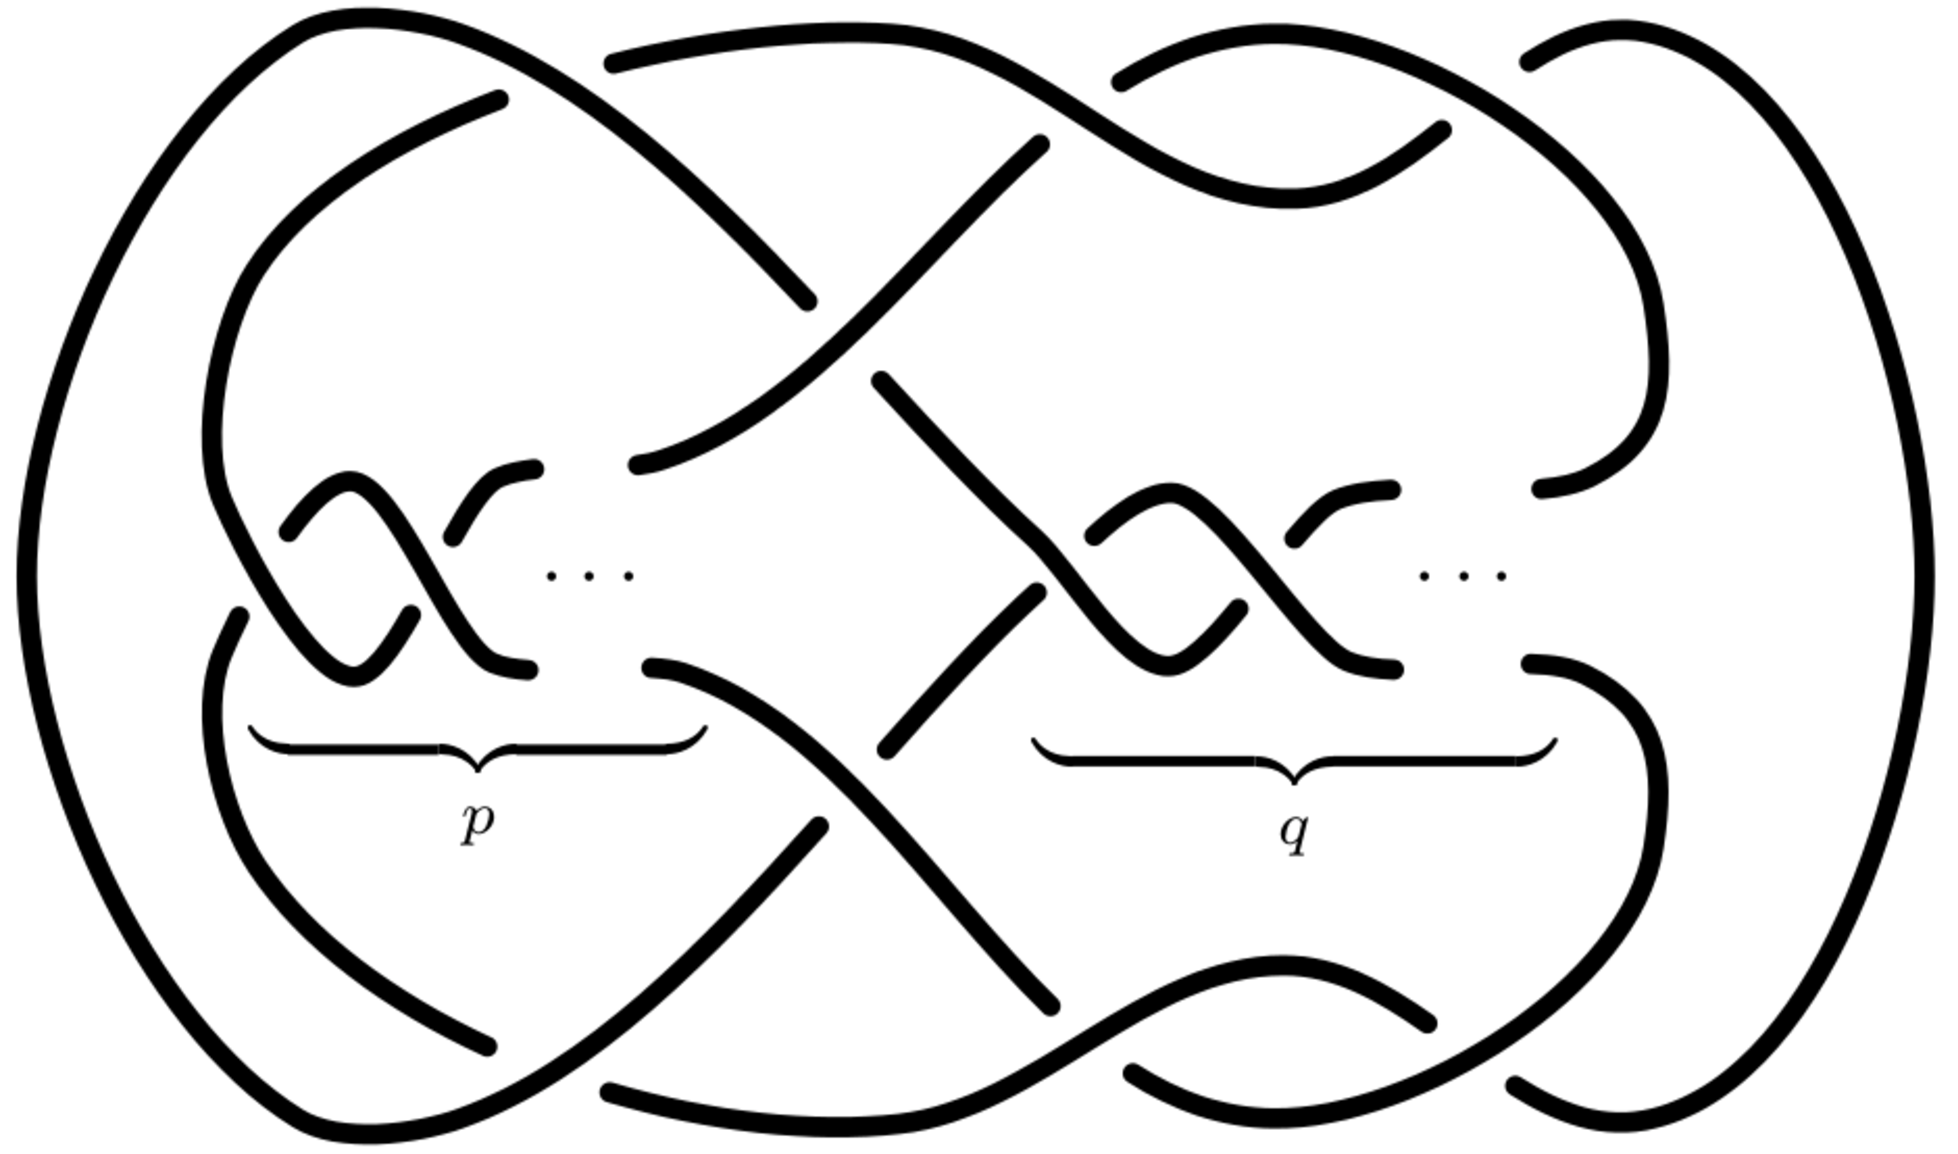
\includegraphics[scale=.37]{kanenobu}
\caption{Kanenobu's knot $K_{p,q}$. Image due to \cite{GreeneWatson}.}
\label{figure:kanenobu}
\end{figure}

\begin{theorem*} The fundamental group $G_n$ of the double branched cover of $K_n$ is not left-orderable.
\label{MAINTHEOREM}
\end{theorem*}

\noindent{} Next, we introduce various definitions and give background on left-orderability.

\subsection{Left-orderability}

%\begin{definition}

%A {\it total order} on a set $X$ is a binary relation $\leq$ satisfying the following for all $x, y, z \in{} X$:
%\begin{enumerate}
%\item $x\leq{}x$ (reflexivity)
%\item $x\leq{}y$ and $y\leq{}x$ implies $x=y$ (anti-symmetry)
%\item $x\leq{}y$ and $y\leq{}z$ implies $x\leq{}z$ (transitivity)
%\item $x\leq{}y$ or $y\leq{}x$ (totality)
%\end{enumerate}
%\end{definition}

\begin{definition}
A group $G$ is {\it left-orderable} if its elements can be given a left-invariant total order. That is, a total order $<$ such that $g<h$ implies $fg<fh$ for all $f, g, h\in{}G$.
\end{definition}

\begin{remark} By convention the trivial group is not left-orderable.
\end{remark}

%\begin{definition} Given a left-orderable group $(G,<)$ we can define a %binary relation $<$ on $G$ in the following way:
%\begin{align*}
%x<y\Leftrightarrow{}x\leq{}y\; \textrm{and} \; x\neq{}y.
%\end{align*}
%\end{definition}
We recall some facts on left-orderable groups from \cite{ClayRolfsen}.

\begin{fact} For some left-orderable group $(G, <)$ we can define {\it a} corresponding relation $>$ in the following way: for $g,h\in{}G$, $g>h$ if and only if $h<g$. This notational convenience will be used frequently.
\end{fact}

\begin{fact} In a left-orderable group G, $1<g$ (``$g$ is positive") if and only if $g^{-1}<1$ (``$g^{-1}$ is negative").
\label{fact:inverses}
\end{fact}
%\begin{proof}
%\begin{align*}
%1<g\Leftrightarrow{}(g^{-1})1<(g^{-1})g\Leftrightarrow{}g^{-1}<1.
%\end{align*}
%\end{proof}

\begin{fact} Transitivity implies that in a left-orderable group products of positive elements are positive and products of negative elements are negative.
\label{1.3LO}
\end{fact}

%\noindent{}We now prove a few useful properties of left-orderable groups.
\begin{proposition} In a left-orderable group $G$, $g\in{}G$ has the same sign as $g^{n}$ for any $n>1$.
\label{proposition:pospowers}
\end{proposition}
\begin{proof} Consequence of Fact \ref{1.3LO}.
%The claim is clear if $g=1$, so we can assume $g<1$. Note that if $g>1$, then we can multiply both sides on the left by $g$ to obtain $g^2>g>1$ and once more to obtain $g^3>g^2>g>1$. Continuing this process shows that $g^n>1$ for any $n>1$ if $g>1$. Similarly, $xg^n<1$ for any $n>1$ if $g<1$. Suppose now that $g>1$ and suppose (for contradiction) that $g^{n}<1$ for some $n>1$. By Proposition~\ref{proposition:inverses}, $g^{-1}<1$ and as noted above, this shows that $g^{n-1}<1$ for any $n>1$. Therefore, $g=(g^{n-1})(g^n)<g^{n-1}<1$, contradicting the fact that $g>1$. A similar proof works when $g<1$.
\end{proof}

\begin{fact} A left-orderable group has no torsion.
\label{fact:torsion}
\end{fact}
%\begin{proof} Suppose G is a left-orderable group, and suppose (for contradiction) that there exists some non-trivial $g\in{}G$ such that $g^{n}=1$ for some $n>1$. We know that either $g>1$ or $g<1$. If $g>1$ then $g^{2}>g>1$ and $g^{3}>g^{2}>g>1$. We can continue this process until we reach $g^{n}$:
%\begin{align*}
%1=g^{n}>g^{n-1}>\cdots{}>g^{2}>g>1.
%\end{align*}
%This is a contradiction. The case when $g<1$ is similar.
%\end{proof}

%\begin{corollary} Every finite group is not left-orderable.
%\end{corollary}
%\begin{proof} Suppose $G$ is a group of finite order. Note: by convention, the trivial group is not left-orderable. We will assume $G$ is non-trivial. Choose $g\in{}G$ such that $g\neq{}1$. The cyclic subgroup $\langle{}g\rangle{}\subset{}G$ is necessarily finite since it is a subgroup of the finite group $G$. This means that $g^{n}=1$ for some $n>1$, and thus $G$ is not left-orderable by Fact~\ref{fact:torsion}.
%\end{proof}

\begin{fact} Let $G$ be a non-trivial group and let $g\in{}G$. There exists a left-ordering $<$ on $G$ such that $g<1$ if and only if there exists a left-ordering $<^\prime$ on $G$ such that $1<^\prime g$.
\label{fact:WLOG}
\end{fact}
%\begin{proof} Suppose there exists a left-ordering $<$ on $G$ such that $g<1$. For $x,y\in{}G$, define $<'$ by:
%\begin{align*}
%x<'y\Leftrightarrow{}y<x.
%\end{align*}
%Because of the properties of $<$, $<'$ is clearly a left-invariant total ordering on $G$. With this definition of $<'$, it is clear that $1<'g$. A similar proof is clear for the converse direction.
%\end{proof}

\noindent{}We can also define left-orderability in a different way:

\begin{proposition} A group $G$ is left-orderable if and only if there exists a subset $P\subset{}G$ such that:
\begin{enumerate}
\item $P\cdot{}P\subset{}P$
\item $P\cap{}P^{-1}=\emptyset{}$
\item $G=P\cup{}P^{-1}\cup{}\{ 1 \}$
\end{enumerate}
\label{proposition:poscone}
\end{proposition}
\begin{proof} Suppose $G$ is left-orderable. Define
\begin{align*}
P=\Set*{g\in{}G}{1<g}.
\end{align*}
Then $P\cdot{}P\subset{}P$ since if $g>1$ and $h>1$ then $gh>g>1$. Therefore, $P$ satisfies the first condition. If $g>1$ then $g^{-1}<1$ and so $P\cap{}P^{-1}=\emptyset{}$. Therefore, $P$ satisfies the second condition. Finally, by the totality of a total ordering, all non-trivial elements in $G$ must be either positive or negative, thus $P\cup{}P^{-1}\cup{}\{ 1 \}$. Therefore, $P$ satisfies the third condition, completing one direction of the proof.\\
\\
Conversely, suppose there exists a subset $P\subset{}G$ satisfying the three conditions of the proposition. Define a left ordering in the following way:
\begin{align*}
g<h\Leftrightarrow{}g^{-1}h\in{}P.
\end{align*}
It is easy to check this defines a left-ordering.
%We will now verify that this is a left-invariant total order. Reflexivity is clear. Anti-symmetry follows from the second condition on $P$, namely  $P\cap{}P^{-1}=\emptyset{}$. This means that it is not possible for both an element and its inverse to be in $P$, and thus for $x,y\in{}G$, $x<y$ and $y<x$ is impossible, so $x\leq{}y$ and $y\leq{}x$ implies $x=y$. Totality is clear from the fact that $G=P\cup{}P^{-1}\cup{}\{ 1 \}$. To prove transitivity, suppose $x,y,z\in{}G$ and $x<y$ and $y<z$. Then $x^{-1}y\in{}P$ and $y^{-1}z\in{}P$. Since $P\cdot{}P\subset{}P$, $(x^{-1}y)(y^{-1}z)=x^{-1}z\in{}P$, and thus $x<z$. Therefore, $<$ is a total order on $G$. Now for $g,h,x\in{}G$, suppose $g<h$. Then:
%\begin{align*}
%g^{-1}h\in{}P\\
%\Rightarrow{}g^{-1}(x^{-1}x)h\in{}P\\
%\Rightarrow{}(g^{-1}x^{-1})(xh)\in{}P\\
%\Rightarrow{}xg<xh.
%\end{align*}
%This shows that $<$ is a left invariant total order, completing the proof.
\end{proof}

\begin{definition} For a group $G$, a subset $P\subset{}G$ satisfying the three conditions of Proposition~\ref{proposition:poscone} is called a {\it positive cone}.
\end{definition}

%\subsection{Double Branch Cover}

%
%\begin{definition}
%A 3-manifold that can be obtained as a union of two solid tori associated by a homeomorphism of their boundaries is called a \emph{lens space}
%\end{definition}
%}

\subsection{Heegaard Floer Homology, L-Spaces, and Lens Spaces}
Heegard Floer homology is an invariant of 3-manifolds, introduced by Ozsv\'{a}th and Szab\'{o} \cite{OzsvathSzabo}. It associates a closed 3-manifold $Y$ a graded vector space over $\mathbb{F}_2$, denoted $\reallywidehat{HF}(Y)$.
\begin{definition}An \emph{L-space} is a rational homology sphere $Y$ with simplest possible Heegaard Floer homology, that is, with
\begin{align*}
rk \reallywidehat{HF}(Y) = |H_1(Y ; \mathbb{Z})|.
\end{align*}
All lens spaces have this property.
\end{definition}

%\subsection{Black and White Graphs, and Greene's Theorem}

%{\begin{definition} The {\it black and white graphs of a knot diagram}: $D\rightarrow{}R^{2}\setminus{}D$
%\label{DefBWD}
%\begin{enumerate}
%\item One vertex for each white/black region
%\item One edge for each crossing
%\item Sign convention for $\mu(x_i,x_j)$
%\begin{figure}[h]
%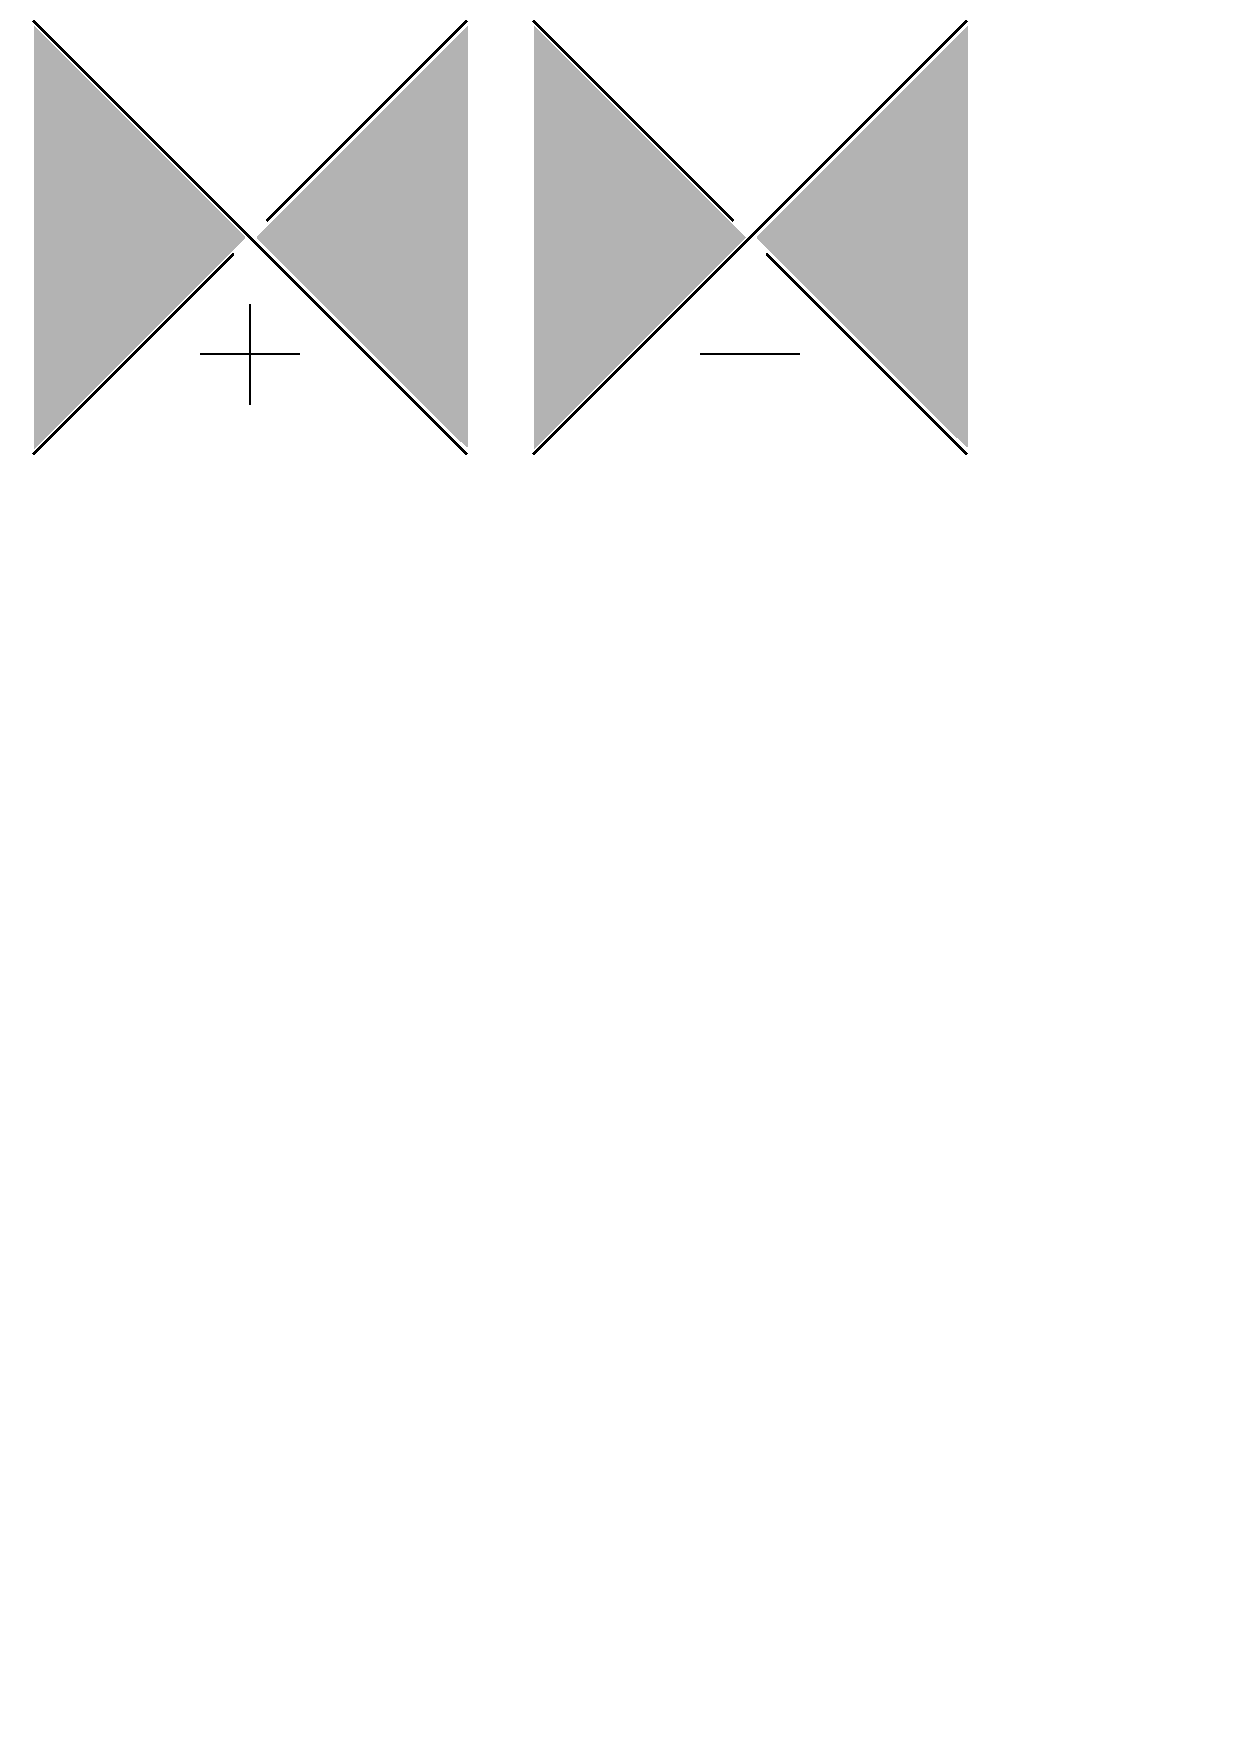
\includegraphics[scale=.37]{signconvention}
%\caption{$\mu(x_i,x_j)$: Sign conventions for the black and white graph.}
%\label{figure:MuCon}
%\end{figure}
%\end{enumerate}
%\end{definition}

%\begin{theorem_greene}
%\label{Greene}
%Let $\Sigma(K)$ denote the double branch cover of some knot K. Then%, and fix a white graph W for some diagram of K. Then $\pi_1(\Sigma(K))\cong{}G_W$:
%\begin{align*}
%\pi_1(\Sigma(K))=\langle{}x_1, x_2,..., x_n:r_1,r_2,...,r_n,x_r\rangle{}
%\end{align*}
%\begin{enumerate}
%\item $x_i$ is a vertex in the white graph of K
%\item $r_i$ is the relator assigned to a vertex
%\item $x_r$ is the root vertex of the white graph of K
%\end{enumerate}
%\begin{align*}
%r_i=(x_i^{-1}x_j)^{\mu(x_i,x_j)}...(x_i^{-1}x_k)^{\mu(x_i,x_k)}.
%\end{align*}
%\end{theorem_greene}

%\begin{figure}[h]
%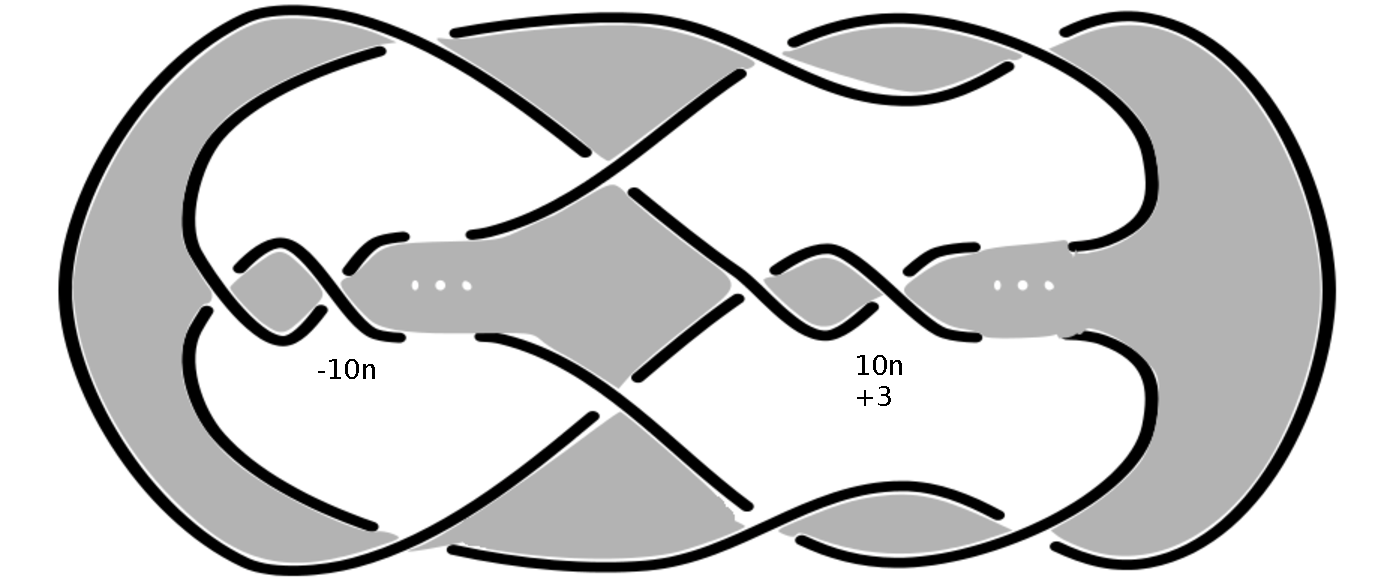
\includegraphics[scale=.5]{KanenobuBW}
%\caption{Checkerboard coloring of $K_{-10n,10n+3}$. Original image due to \cite{GreeneWatson}.}
%\label{figure:kanenobuCheckboard}
%\end{figure}

%\begin{figure}[h]
%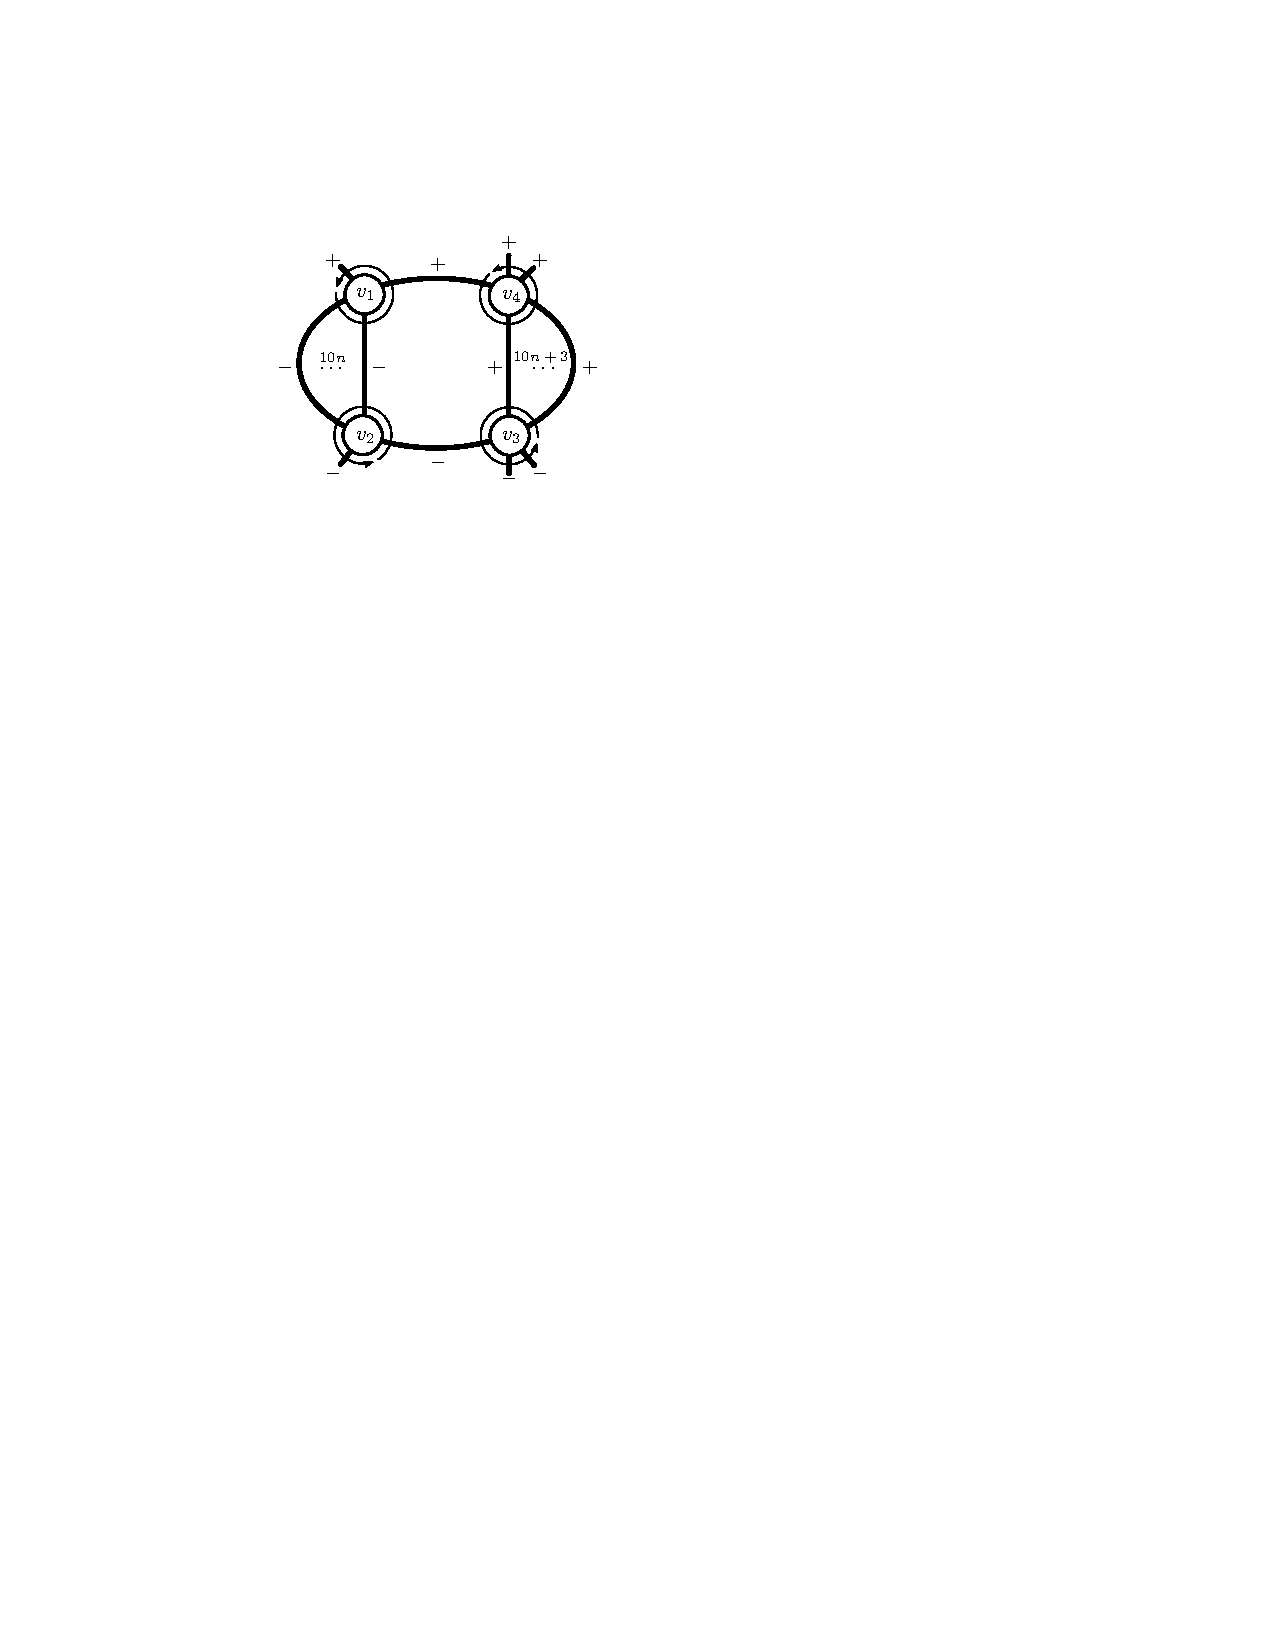
\includegraphics[scale=2]{KanenobuWG}
%\caption{White graph for $K_{-10n,10n+3}$. Note that edges which appear not to connect to any vertices actually connect to the root vertex, which is not shown. Image due to \cite{GreeneWatson}.}
%\label{figure:kanenobuWG}
%\end{figure}

%The checkerboard coloring of $K_n$ is shown in Figure~\ref{figure:kanenobuCheckboard}. Using this, and Following the procedures outlined in Definition~\ref{DefBWD}, we have Figure \ref{figure:kanenobuWG}, and by Greene's Theorem, we have that for all $n\geq{}0$ from

\subsection{Automated Proofs}
Several of the proofs for lemmas and propositions in this paper were generated by a computer program we created for the task. We will now briefly describe the algorithm our program employs, as it could be useful for future work in disproving the left-orderability of certain groups. Our program is similar to the program described in \cite[Section 8]{CalegariDunfield}.

For the proof that $G_n$ is not left-orderable, we argue by contradiction. That is, we assume that $G_n$ is left-orderable, thus for any left-ordering on $G_n$, there must exist a positive cone $P\subset{}G_n$. Based on Fact~\ref{fact:WLOG}, we can proceed under the assumption that $b^{-1}a\in{}P$, and then find additional elements of $G_n$ that must be contained in such a positive cone. With the addition of enough elements, we can in many cases reach a contradiction.

In order to accomplish this, the program takes two inputs:
\begin{enumerate}
\item A set $Q\subset{}P$ of elements that have been proven (either in previous iterations of the program, or by hand) to be contained in $P$, including $b^{-1}a$. This set will grow during the execution of the program, but we will ensure that it always is a subset of $P$, so $Q$ has the property inherited from $P$ that $1\not\in Q^{*}$, where $Q^*$ is the semigroup generated by $Q$. 
\item A subset $I$ of all words that we know are equal to the identity based on the group relations of $G_n$, closed under inversion and cyclic permutation. See (\ref{intro:cyclic}) for an example of what is meant by cyclic permutation.
\end{enumerate}
\begin{remark}
Words that are equal to the identity are henceforth referred to as identities.
\end{remark}
The four group relations of $G_n$ are obvious examples of identities. To give another example, Lemma~\ref{lemma:eq5} shows that $d^{-1}a^{2}b^{-2}c$ is also an identity. The cyclic permutations of this identity would be:
\begin{align}
\{d^{-1}a^{2}b^{-2}c,\; cd^{-1}a^{2}b^{-2},\; b^{-1}cd^{-1}a^{2}b^{-1},\nonumber{}\\
b^{-2}cd^{-1}a^{2},\; ab^{-2}cd^{-1}a,\; a^{2}b^{-2}cd^{-1}\}. \label{intro:cyclic}
\end{align}

% For any such left-ordering, we consider the set $A=\{P\subset{}G_n\mid{}P \textrm{ is a positive cone and } b^{-1}a\in{}P\}$. We then show that $A$ is empty by reaching contradictions for all such $P$.


%$P=\{x\in G_n|1<x\}$, which satisfies the previously described properties of a positive cone. Thus, proving that such a $P$ doesn't satisfy the properties of a positive cone is equivalent to showing $G_n$ is not left-orderable.

%The program then performs two sorts of checks:

%Maybe we should skip these next two paragraphs entirely? These talk about checking for internal consistancy of the positive cone and list of identities, but the way I worded the above makes it seem (as I think it should) that the elements of the positive cone are known absolutely to be positive and that identities are also "infalible". It makes more sense, I think, to just talk about how the program addresses elements of unknown sign.

%First, since we know that $P$ is closed under the group operation and that $P\cap P^{-1}=\emptyset$, the program checks if the inverse of any element in $P$ is also in $P$, that is, that it can be expressed as a product of elements in $P$. If it can, then this element is contained in both $P$ and $P^{-1}$, a contradiction.

%Second, the program checks if any of the identities (including their inverses and conjugates, which are also identities) can be expressed as a combination of elements in the positive cone. If any of them can, then we reach the conclusion that the identity is positive, again a contradiction.

%If neither the unknown sign element nor its inverse causes a contradiction,

Pseudocode for a simplified version of the program follows, where $A^*$ denotes the semigroup generated by the elements of $A$.\\

\begin{algorithmic}
\LOOP
\STATE $x\gets$ next nontrivial element of unknown sign
  \IF {$I\cap{}(Q\cup{}\{x\})^*=\emptyset{}$ \AND $I\cap{}(Q\cup{}\{x^{-1}\})^*\neq{\emptyset{}}$}
    \STATE {\textbf{add} $x$ \textbf{to} $Q$}
    \PRINT {$x$ added to positive list}
  \ELSIF {$I\cap{}(Q\cup{}\{x\})^*\neq{}\emptyset{}$ \AND $I\cap{}(Q\cup{}\{x^{-1}\})^*={\emptyset{}}$}
    \STATE {\textbf{add} $x^{-1}$ \textbf{to} $Q$}
    \PRINT {$x^{-1}$ added to positive list}
  \ELSIF {$I\cap{}(Q\cup{}\{x\})^*\neq{}\emptyset{}$ \AND $I\cap{}(Q\cup{}\{x^{-1}\})^*\neq{}{\emptyset{}}$}
    \PRINT {$x$ causes a contradiction}
    \STATE {\textbf{program halts}}
  \ENDIF
\ENDLOOP
\end{algorithmic}
$\;$\\
The ``next nontrivial element of unknown sign" from line 2 can either be user-input or computer-generated. Since there are infinite elements of unknown sign, we (or the computer) give preference to those elements with lowest word length, e.g. $c^{-1}d$ before $c^{-1}d^2$.

Within the program's \textbf{if} statements, we compute the intersection between the finite set $I$ and infinite semigroups generated by $Q\cup{}\{x\}$ or $Q\cup{}\{x^{-1}\}$. This is possible in finitely many operations because $I$ is finite and the semigroup is finitely generated. We use a method similar to using a deterministic finite automaton with the finitely generated semigroup as a language to check elements in $I$.

%The version of the algorithm that we employed keeps track of the reasoning behind the addition of an element to the positive list, which we then use in our proofs.



%begin{algorithmic}
%while true
%  $x\gets$ next element of unknown sign
%  if $I\cap{}(Q\cup{}x)^*=\emptyset{}$ \AND $I\cap{}(Q\cup{}x^{-1})^*\neq{\emptyset{}}$
%    \PRINT $I\cap{}(Q\cup{}q^{-1})^*$
%    add $x$ to $Q$
%  else if $I\cap{}(Q\cup{}x)^*\neq{}\emptyset{}$ \AND $I\cap{}(Q\cup{}x^{-1})^*={\emptyse%t{}}$
%    \PRINT $I\cap{}(Q\cup{}x)^*$
%    add $x^{-1}$ to $Q$
%  else if $I\cap{}(Q\cup{}x)^*=\emptyset{}$ \AND $I\cap{}(Q\cup{}x^{-1})^*=\emptyset{}$
%    \PRINT $I\cap{}(Q\cup{}q^{-1})^*$
%    \PRINT $I\cap{}(Q\cup{}q^{-1})^*$
%    STOP
%\end{algorithmic}

%For the elements whose sign we do not know (in ascending order by word length after accounting for cancellations), the program gets the first of these elements, call it $q$, and tries two cases\textemdash{}Case 1: $q$ is positive, Case 2: $q^{-1}$ is positive

%checks for any of the [[[[two mentioned contradictions]]]]. It then replaces this recently-added element in the positive cone list with the inverse of the same element and again checks for contradictions.

%If none of these two elements (neither the unknown-sign element nor its inverse) causes a contradiction when assumed to be positive, the program gains no information, so it tries the next item of unknown sign.

%If one of the two causes a contradiction, the program adds the inverse permanently to the positive cone and continues with another element we do not know the sign of.

%Finally, if both the element and its inverse cause a contradiction, the program reaches a general contradiction, and it halts.

\subsection{Outline}
The paper is organized as follows. In Section~\ref{section:G_0}, we provide a proof that $G_0$ is not left-orderable. The case when $n=0$ is addressed separately because the proof for $n>0$ does not hold when $n=0$. The remainder of the paper is then devoted to a proof for the cases $n>0$. To facilitate the proof, we consider sixteen cases (see Table~\ref{table:casesAll}) based on the signs of the four generators of $G_n$ and disprove left-orderability in each. In Section~\ref{section:identityProofs} we show that the four generators of $G_n$ are non-trivial and distinct, justifying the totality of the sixteen cases we will address. In Section~\ref{section:generalLemmas} we prove lemmas that hold in all cases and that will be useful for later proofs. With these tools, left-orderability is straightforward to disprove in eleven of the sixteen cases, and we address these in Section~\ref{section:manyCases}. We disprove left-orderability in Cases 3, 4, 8, 1, and 16  in Sections~\ref{section:case3},~\ref{section:case4},~\ref{section:case8},~\ref{section:case1}, and~\ref{section:case16} respectively.

\subsection{Acknowledgements} We would like to thank Jennifer Hom and Kristen Hendricks for their generous advice throughout the project, Columbia University's REU Summer Program for providing us the opportunity to work together, Adam Clay and Dale Rolfsen for sharing their notes on ``Ordered Groups and Topology," and Tye Lidman and Liam Watson for suggesting this problem. We would also like to thank Tye Lidman and the anonymous reviewers at the Journal of Knot Theory and Its Ramifications for comments on earlier drafts of this paper. Finally, we would like to thank the National Science Foundation---Fabian Doria Medina was partly supported by NSF grant DMS-1149800.

\section{Proof that $G_0$ is not left-orderable}
\label{section:G_0}
We start by proving that $G_0$ is not left-orderable, as the proof uses a different approach than the general case $n\geq1$
\begin{lemma} $G_0$ is isomorphic to $\langle x,\; y\mid{}(x^{-2}y^{2})^{3}=x^{5}=y^{5} \rangle$.
\end{lemma}
\begin{proof} When $n=0$, we have:
\begin{align*}
G_0=\langle a,\; b,\; c,\; d \mid{} d^{-1}a^{2},\; b^{-2}c,\; (d^{-1}c)^{3}c^{-1}bc^{-2},\; d^{2}a^{-1}d(c^{-1}d)^{3} \rangle.
\end{align*}
The first two relations show that $a^{2}=d$ and $b^{2}=c$, thus we can rewrite the presentation using only $a$ and $b$ as generators:
\begin{align*}
G_0&=\langle a,\;b\mid{} (a^{-2}b^{2})^{3}b^{-2}bb^{-4},\; a^{4}a^{-1}a^{2}(b^{-2}a^{2})^{3} \rangle\\
G_0&=\langle a,\;b\mid{} (b^{-2}a^{2})^{3}=b^{-5},\; a^{5}(b^{-2}a^{2})^{3} \rangle\\
G_0&=\langle a,\;b\mid{} (b^{-2}a^{2})^{3}=b^{-5},\; a^{5}b^{-5} \rangle\\
G_0&=\langle a,\;b\mid{} (a^{-2}b^{2})^{3}=a^{5}=b^{5} \rangle.\qedhere
\end{align*}
\end{proof}

\begin{lemma} Both $x^{5}$ and $y^{5}$ commute with all elements in $G_0$.
\label{lemma:G_0:center}
\end{lemma}
\begin{proof} Since we can change $x^5$ to $y^5$ and back as necessary, it is clear that both $x^5$ and $y^5$ commute with $x$, $y$, $x^{-1}$, and $y^{-1}$ and therefore with any element of $G_0$.

%Let $w\in{}G_0$ be any word. We will show that $wx^{5}=x^{5}w$ and similarly with $y^{5}$. The elements $x$ and $y$ generate $G_0$, so $w$ can be expressed as some word in $x$ and $y$, that is:
%\begin{align*}
%w=x^{n_0}y^{n_1}x^{n_2}y^{n_3}\cdots{}x^{n_{N-2}}y^{n_{N-1}}x^{n_N}.
%\end{align*}
%Where all $n_i$ are non-zero integers except $n_0$ and $n_N$ which may be zero. Then:
%\begin{align*}
%wx^{5}&=x^{n_0}y^{n_1}x^{n_2}y^{n_3}\cdots{}x^{n_{N-2}}y^{n_{N-1}}x^{n_N}x^{5}\hfil\\
%&=x^{n_0}y^{n_1}x^{n_2}y^{n_3}\cdots{}x^{n_{N-2}}y^{n_{N-1}}x^{n_N+5}\hfil\\
%&=x^{n_0}y^{n_1}x^{n_2}y^{n_3}\cdots{}x^{n_{N-2}}y^{n_{N-1}}x^{5}x^{n_N}\hfil\\
%&=x^{n_0}y^{n_1}x^{n_2}y^{n_3}\cdots{}x^{n_{N-2}}y^{n_{N-1}}y^{5}x^{n_N}\hfil\\
%&=x^{n_0}y^{n_1}x^{n_2}y^{n_3}\cdots{}x^{n_{N-2}}y^{n_{N-1}+5}x^{n_N}\hfil\\
%&=x^{n_0}y^{n_1}x^{n_2}y^{n_3}\cdots{}x^{n_{N-2}}y^{5}y^{n_{N-1}}x^{n_N}\hfil\\
%&=x^{n_0}y^{n_1}x^{n_2}y^{n_3}\cdots{}x^{n_{N-2}}x^{5}y^{n_{N-1}}x^{n_N}\hfil\\
%\intertext{\center $\vdots{}$}
%\setbox0\hbox{$\cdots{}$}\mathrel{\makebox[\wd0]{\hfil\vdots\hfil}}\\
%&\hspace{80pt} \vdots{}\\
%&=x^{n_0}x^{5}y^{n_1}x^{n_2}y^{n_3}\cdots{}x^{n_{N-2}}y^{n_{N-1}}x^{n_N}\hfil\\
%&=x^{n_0+5}y^{n_1}x^{n_2}y^{n_3}\cdots{}x^{n_{N-2}}y^{n_{N-1}}x^{n_N}\hfil\\
%&=x^{5}x^{n_0}y^{n_1}x^{n_2}y^{n_3}\cdots{}x^{n_{N-2}}y^{n_{N-1}}x^{n_N}\hfil\\
%wx^{5}&=x^{5}w.
%\end{align*}
%A similar proof is clear for $y^{5}$.
\end{proof}

\begin{lemma} If $G_0$ is left-orderable, then $wx^{n}w^{-1}$ has the same sign as $x$ for any $w\in{}G_0$ and for any $n\geq{}1$. Similarly, $wy^{n}w^{-1}$ has the same sign as $y$ for any $w\in{}G_0$ and for any $n\geq{}1$.
\label{lemma:G_0:conjugates}
\end{lemma}
\begin{proof} Suppose $G_0$ is left-orderable. We know by Lemma~\ref{lemma:G_0:center} that for any $w\in{}G_0$:
\begin{align*}
wx^{5}w^{-1}=ww^{-1}x^{5}=x^{5}.
\end{align*}
By Proposition~\ref{proposition:pospowers}, $x^5$ has the same sign as $x$, and thus $wx^{5}w^{-1}$ has the same sign as $x$. But $wx^{5}w^{-1}=(wxw^{-1})^{5}$, and so by Proposition~\ref{proposition:pospowers} $wxw^{-1}$ has the same sign as $wx^{5}w^{-1}$ and therefore has the same sign as $x$. A similar proof works for $y$.
\end{proof}

\begin{lemma} If $G_0$ is left-orderable and $x>1$, then $x^{-2}y^{2}>1$.
\label{lemma:G_0:XXyy}
\end{lemma}
\begin{proof}
Suppose $G_0$ is left-orderable and suppose $x>1$. Then $x^5>1$ and $(x^{-2}y^2)^{3}>1$ since $(x^{-2}y^2)^{3}=x^5$. By Proposition~\ref{proposition:pospowers} this shows that $x^{-2}y^2>1$.
\end{proof}

\begin{proposition}
The group $G_0=\langle x,\; y \mid{} (x^{-2}y^{2})^{3}=x^{5}=y^{5} \rangle$ is not left-orderable.
\label{propG0}
\end{proposition}
\begin{proof} Suppose (for contradiction) that $G_0$ is left-orderable. First note that if $x=1$, then $y^5=1$. Then either $y=1$ as well and $G_0$ is trivial, or $y\neq{}1$ and $G_0$ has torsion and is therefore not left-orderable by Fact~\ref{fact:torsion}, a contradiction. Thus by Fact~\ref{fact:WLOG} we can assume without loss of generality that $x>1$. Note that $x>1$ implies $x^5=y^5>1$ which implies $y>1$ by Proposition~\ref{proposition:pospowers}. Starting with the group relation, we have:
\begin{align}
x^{-2}y^{2}x^{-2}y^{2}x^{-2}y^{2}&=y^{5}\nonumber{}\\
x^{-2}y^{2}x^{-2}y^{2}x^{-2}&=y^{3}\nonumber{}\\
x^{-2}y^{2}x^{-2}y^{2}x^{2}&=y^{3}x^{4}\nonumber{}\\
x^{-2}y^{2}x^{-2}y^{2}x^{2}&=x^{5}y^{3}x^{-1}
\label{x5center}\\
y^{2}x^{-2}y^{2}x^{2} & =x^{7}y^{3}x^{-1}\nonumber{}\\
y^{-2}x^{-2}y^{2}x^{2} & =y^{-4}x^{7}y^{3}x^{-1}\nonumber{}\\
[x^{-2}y^{-2}]x^{-2}[y^{2}x^{2}] & =x^{-2}y^{-4}x^{5}x^{2}y^{3}x^{-1}\nonumber{}\\
& =x^{-2}yx^{2}y^{3}x^{-1}
\label{x5=y5}\\
[(x^{-1})x^{-2}y^{-2}]x^{-2}[y^{2}x^{2}(x)] & =(x^{-1})x^{-2}yx^{2}y^{3}x^{-1}(x)\nonumber{}\\
[(y^{3})x^{-3}y^{-2}]x^{-2}[y^{2}x^{3}(y^{-3})] & =(y^{3})x^{-3}yx^{2}(y^{3}y^{-3})\nonumber{}\\
[(x^{-2})y^{3}x^{-3}y^{-2}]x^{-2}[y^{2}x^{3}y^{-3}(x^{2})] & =(x^{-2})y^{3}x^{-3}yx^{2}(x^{2})\nonumber{}\\
[x^{-2}y^{3}x^{-3}y^{-2}] x^{-2} [x^{-2}y^{3}x^{-3}y^{-2}]^{-1} & =[x^{-2}y^{2}]y[(x^{-3})y(x^{3})]x.
\label{PFcontraG0}
\end{align}
Where for (\ref{x5center}) we have used the fact (shown in Lemma~\ref{lemma:G_0:center}) that $x^5$ commutes with any element of $G_0$, for (\ref{x5=y5}) we have used the group relation $x^{5}=y^{5}$. Now in (\ref{PFcontraG0}), the right expression must be positive since $x>1$, $y>1$, $x^{-2}y^{2}>1$ by Lemma~\ref{lemma:G_0:XXyy}, and $(x^{-3})y(x^{3})>1$ by Lemma~\ref{lemma:G_0:conjugates}. However, the expression on the left is negative by Lemma~\ref{lemma:G_0:conjugates} since it is of the form $(wx^{-1}w^{-1})^{2}$ for some $w\in{}G_0$. This is a contradiction.
\end{proof}

\begin{remark}
An alternative proof of Proposition \ref{propG0} follows from the fact that $K_0$ is a Montesino knot, and hence $\Sigma{}(K_0)$ is a Seifert fibered space. Proposition \ref{propG0} then follows from \cite[Theorem 4]{BoyerGordonWatson}.
\end{remark}

\section{Non-triviality of the four generators and $b^{-1}a$}
\label{section:identityProofs}

\noindent{}Recall that
\begin{align*}
G_n=\langle a,\; b,\; c,\; d \mid{} &(a^{-1}b)^{10n}d^{-1}a^{2},\; b^{-2}c(b^{-1}a)^{10n},\\
&(d^{-1}c)^{10n+3}c^{-1}bc^{-2},\; d^{2}a^{-1}d(c^{-1}d)^{10n+3} \rangle
\end{align*}
for integers $n\geq{}0$.

\vspace{10pt}

\noindent{}We will assume $G_n$ is left-orderable and then reach a contradiction. By Fact~\ref{fact:WLOG}, we can assume without loss of generality that $b^{-1}a\geq1$.

\begin{proposition}
If $G_n$ is left-orderable, then $b^{-1}a\neq1$.
\label{proposition:id:Ba}
\end{proposition}
\begin{proof}
Suppose $G_n$ is left-orderable, and suppose (for contradiction) that $b^{-1}a=1$. By the first group relation:
\begin{align}
(a^{-1}b)^{10n}d^{-1}a^{2} & =1\nonumber\\
\Rightarrow{}(b^{-1}a)^{-10n}d^{-1}a^{2} & =1\nonumber\\
\Rightarrow{} d^{-1}a^{2} & =1\nonumber\\
\Rightarrow{} d & =a^{2}.\nonumber
\end{align}
Similarly, by the second group relation:
\begin{align}
b^{-2}c(b^{-1}a)^{10n} & =1\nonumber\\
\Rightarrow b^{-2}c & =1\nonumber\\
\Rightarrow c & =b^{2}.\nonumber
\end{align}
We know $b^{-1}a=1$, which implies $a=b$. Combining these results, we find
\begin{align}
c & =b^{2}\nonumber\\
 & =a^{2}\nonumber\\
 & =d.\nonumber
\end{align}
We now apply our recently obtained equalities $b=a$, $c=a^{2}$, and $d=a^{2}$ to the definition of $G_{n}$ to get:
\begin{align}
G_{n}= & \langle a,a,a^{2},a^{2}\mid{}(a^{-1}[a])^{10n}[a^{2}]^{-1}a^{2},\;[a]^{-2}[a^{2}]([a]^{-1}a)^{10n},\nonumber\\
 & ([a^{2}]^{-1}[a^{2}])^{10n+3}[a^{2}]^{-1}[a][a^{2}]^{-2},\;[a^{2}]^{2}a^{-1}[a^{2}]([a^{2}]^{-1}[a^{2}])^{10n+3}\rangle\nonumber\\
= & \langle a\mid{}1,\;1,\; a^{-5},\; a^{5}\rangle\nonumber\\
\cong & \mathbb{Z}/5\mathbb{Z}\nonumber
\end{align}
which is a nontrivial finite group and thus not left-orderable. This is a contradiction, therefore $b^{-1}a\neq{}1$.
\end{proof}

\noindent{}Because of Proposition~\ref{proposition:id:Ba}, we can assume (without loss of generality) that $b^{-1}a>1$. We will now show that if $G_n$ is left-orderable, then all of the generators of $G_n$ are non-trivial.

\begin{proposition}
If $G_n$ is left-orderable, then $c\neq d$.
\label{proposition:id:Dc}
\end{proposition}
\begin{proof} Suppose $G_n$ is left-orderable, and suppose (for contradiction) that $c=d$. By the third group relation:
\begin{align}
(d^{-1}c)^{10n+3}c^{-1}bc^{-2} & =1\nonumber\\
\Rightarrow(c^{-1}c)^{10n+3}c^{-1}bc^{-2} & =1\nonumber\\
\Rightarrow b & =c^{3}.\nonumber
\end{align}
Similarly, by the fourth group relation:
\begin{align}
d^{2}a^{-1}d(c^{-1}d)^{10n+3} & =1\nonumber\\
\Rightarrow c^{2}a^{-1}c(c^{-1}c)^{10n+3} & =1\nonumber\\
\Rightarrow a & =c^{3}.\nonumber
\end{align}
Combining these results, we get that $a=b$, or equivalently $b^{-1}a=1$,
but we know from Proposition~\ref{proposition:id:Ba} that $b^{-1}a\neq1$. This is a contradiction, therefore $c\neq{}d$.
\end{proof}

\begin{proposition}
If $G_n$ is left-orderable, then $a\neq1$.
\label{proposition:id:a}
\end{proposition}
\begin{proof} Suppose $G_n$ is left-orderable, and suppose (for contradiction) that $a=1$. By the first group relation:
\begin{align}
([1]^{-1}b)^{10n}d^{-1}[1]^{2} & =1\nonumber\\
\Rightarrow b^{10n}d^{-1} & =1\nonumber\\
\Rightarrow d & =b^{10n},\label{proposition:id:a:1}
\end{align}
and by the second group relation:
\begin{align}
b^{-2}c(b^{-1}[1])^{10n} & =1\nonumber\\
\Rightarrow b^{-2}cb^{-10n} & =1\nonumber\\
\Rightarrow c & =b^{10n+2}.\label{proposition:id:a:2}
\end{align}
Using (\ref{proposition:id:a:1}) and (\ref{proposition:id:a:2}), we substitute for $c$ and $d$ in the third group relation:
\begin{align}
([b^{10n}]^{-1}[b^{10n+2}])^{10n+3}[b^{10n+2}]^{-1}b[b^{10n+2}]^{-2} & =1\nonumber\\
\Rightarrow(b^{2})^{10n+3}b^{-10n-2}bb^{-20n-4} & =1\nonumber\\
\Rightarrow b^{1-10n} & =1.\nonumber
\end{align}
Which means that $b$ has finite order. Furthermore, we know $b\neq1$
because $a=1$ and $b^{-1}a\neq1$ by Proposition~\ref{proposition:id:Ba}, so $G_{n}$ has torsion for any $n$ and is therefore not left-orderable by Fact~\ref{fact:torsion}. This is a contradiction, therefore $a\neq{}1$.
\end{proof}

\begin{proposition}
If $G_n$ is left-orderable, then $b\neq1$.
\label{proposition:id:b}
\end{proposition}
\begin{proof}
Suppose $G_n$ is left-orderable, and suppose (for contradiction) that $b=1$. By the first group relation:
\begin{align}
(a{}^{-1}[1])^{10n}d^{-1}a^{2} & =1\nonumber\\
\Rightarrow a^{-10n}d^{-1}a^{2} & =1\nonumber\\
\Rightarrow d & =a^{-10n+2},\label{proposition:id:b:1}
\end{align}
and by the second group relation:
\begin{align}
[1]^{-2}c([1]^{-1}a)^{10n} & =1\nonumber\\
\Rightarrow ca^{10n} & =1\nonumber\\
\Rightarrow c & =a^{-10n}.\label{proposition:id:b:2}
\end{align}
Using (\ref{proposition:id:b:1}) and (\ref{proposition:id:b:2}), we substitute for $c$ and $d$ in the third group relation:
\begin{align}
([a^{-10n+2}]^{-1}[a^{-10n}])^{10n+3}[a^{-10n}]^{-1}[1][a^{-10n}]^{-2} & =1\nonumber\\
\Rightarrow(a^{-2})^{10n+3}a^{30n} & =1\nonumber\\
\Rightarrow a^{10n-6} & =1.\nonumber
\end{align}
By Proposition~\ref{proposition:id:a}, $a\neq1$, so this shows that $G_{n}$
has torsion for any choice of $n$. Therefore $G_{n}$ is not left-orderable by Fact~\ref{fact:torsion}. This is a contradiction, therefore $b\neq{}1$.
\end{proof}

\begin{proposition}
If $G_n$ is left-orderable, then $c\neq1$.
\label{proposition:id:c}
\end{proposition}
\begin{proof} Suppose $G_n$ is left-orderable, and suppose (for contradiction) that $c=1$. By the third group relation, we have:
\begin{align}
(d^{-1}[1])^{10n+3}[1]^{-1}b[1]^{-2} & =1\nonumber\\
\Rightarrow d^{-10n-3}b & =1\nonumber\\
\Rightarrow b & =d^{10n+3}.\label{proposition:id:c:1}
\end{align}
Similarly, by the fourth group relation:
\begin{align}
d^{2}a^{-1}d([1]d)^{10n+3} & =1\nonumber\\
\Rightarrow a^{-1}d^{10n+6} & =1\nonumber\\
\Rightarrow a & =d^{10n+6}.\label{proposition:id:c:2}
\end{align}
Using (\ref{proposition:id:c:1}) and (\ref{proposition:id:c:2}), we substitute for $a$ and $b$ in the first group relation:
\begin{align}
([d^{10n+6}]^{-1}[d^{10n+3}])^{10n}d^{-1}[d^{10n+6}]^{2} & =1\nonumber\\
\Rightarrow(d^{-3})^{10n}d^{20n+11} & =1\nonumber\\
d^{-10n+11} & =1.\label{proposition:id:c:3}
\end{align}
We know that $d\neq1$ since $c=1$ and $c\neq d$ by Proposition~\ref{proposition:id:Dc}. Thus $G_{n}$ has torsion for any $n>1$, and is therefore not left-orderable by Fact~\ref{fact:torsion}. Similarly, if $n=1$ then (\ref{proposition:id:c:3}) implies $d=1$. In both cases there is a contradiction, therefore $c\neq{}1$.
\end{proof}

%------------------------- d != 1 ------------------------
\begin{proposition}
If $G_n$ is left-orderable, then $d\neq1$.
\label{proposition:id:d}
\end{proposition}
\begin{proof} Suppose $G_n$ is left-orderable, and suppose (for contradiction) that $d=1$. By the third group relation, we have:
\begin{align}
([1]^{-1}c)^{10n+3}c^{-1}bc^{-2} & =1\nonumber\\
b & =c^{-10n}.\label{proposition:id:d:1}
\end{align}
Similarly, by the fourth group relation:
\begin{align}
[1]^{2}a^{-1}[1](c^{-1}[1])^{10n+3} & =1\nonumber\\
a & =c^{-10n-3}.\label{proposition:id:d:2}
\end{align}
Using (\ref{proposition:id:d:1}) and (\ref{proposition:id:d:2}), we substitute for $a$ and $b$ in the first group relation:
\begin{align}
([c^{-10n-3}]^{-1}[c^{-10n}])^{10n}[c^{-10n-3}]^{2} & =1\nonumber\\
(c^{3})^{10n}(c^{-20n-6}) & =1\nonumber\\
c^{10n-6} & =1.\nonumber
\end{align}
By Proposition~\ref{proposition:id:c}, we know that $c\neq1$, so this shows that $G_{n}$ has torsion for any choice of $n$ and is therefore not left-orderable by Fact~\ref{fact:torsion}. This is a contradiction, therefore $d\neq{}1$.
\end{proof}

\noindent{}With four (non-trivial) group generators there are 16 possible cases for the signs of each of the generators that must be considered (see Table~\ref{table:casesAll}). We will disprove each of these cases.



\begin{table}[ht]
\begin{center}
\begin{tabular}{l | l | l | l | l}
Case\hspace{10 pt} & $a$\hspace{10 pt} & $b$\hspace{10 pt} & $c$\hspace{10 pt} & $d$\hspace{10 pt} \\\hline\hline
1 & $+$ & $+$ & $+$ & $+$ \\\hline
2 & $+$ & $+$ & $+$ & $-$ \\\hline
3 & $+$ & $+$ & $-$ & $+$ \\\hline
4 & $+$ & $+$ & $-$ & $-$ \\\hline
5 & $+$ & $-$ & $+$ & $+$ \\\hline
6 & $+$ & $-$ & $+$ & $-$ \\\hline
7 & $+$ & $-$ & $-$ & $+$ \\\hline
8 & $+$ & $-$ & $-$ & $-$ \\\hline
9 & $-$ & $+$ & $+$ & $+$ \\\hline
10 & $-$ & $+$ & $+$ & $-$ \\\hline
11 & $-$ & $+$ & $-$ & $+$ \\\hline
12 & $-$ & $+$ & $-$ & $-$ \\\hline
13 & $-$ & $-$ & $+$ & $+$ \\\hline
14 & $-$ & $-$ & $+$ & $-$ \\\hline
15 & $-$ & $-$ & $-$ & $+$ \\\hline
16 & $-$ & $-$ & $-$ & $-$ 
\end{tabular}
\end{center}
\caption{The 16 possible cases with 4 generators}
\label{table:casesAll}
\end{table}

\section{General Lemmas}
\label{section:generalLemmas}

\noindent{}First we prove some lemmas that will be used later. These lemmas are true for all cases listed in Table~\ref{table:casesAll}.

\begin{lemma} In $G_n$, $d^{-1}a^{2}=c^{-1}b^{2}$.
\label{lemma:eq5}
\end{lemma}
\begin{proof} The first group relation for $G_n$ can be rearranged as follows:
\begin{align}
(a^{-1}b)^{10n}d^{-1}a^{2}&=1\nonumber{}\\
\Rightarrow{}(b^{-1}a)^{10n}&=d^{-1}a^{2},\label{eq1:2}
\end{align}
and the second group relation can be rearranged as follows:
\begin{align}
b^{-2}c(b^{-1}a)^{10n}&=1\nonumber{}\\
\Rightarrow{}(b^{-1}a)^{10n}&=c^{-1}b^{2}.\label{eq2:2}
\end{align}
This shows that:
\begin{align*}
d^{-1}a^{2}&=c^{-1}b^{2}.\qedhere
\end{align*}
\end{proof}

\begin{corollary} In $G_n$, $a^{2}b^{-2}=dc^{-1}$.
\label{corollary:eq6}
\end{corollary}
\begin{proof}By Lemma~\ref{lemma:eq5} we know:
\begin{align*}
d^{-1}a^{2}&=c^{-1}b^{2}\\
\Rightarrow{}a^{2}b^{-2}&=dc^{-1}.\qedhere
\end{align*}
\end{proof}

\begin{lemma} In $G_n$, $d^{2}a^{-1}d=c^{2}b^{-1}c$.
\label{lemma:eq7}
\end{lemma}
\begin{proof}
The third group relation for $G_n$ can be rearranged as follows:
\begin{align*}
(d^{-1}c)^{10n+3}c^{-1}bc^{-2}&=1\\
\Rightarrow{}(d^{-1}c)^{10n+3}&=c^{2}b^{-1}c,
\end{align*}
and the fourth group relation can be rearranged as follows:
\begin{align*}
d^{2}a^{-1}d(c^{-1}d)^{10n+3}&=1\\
\Rightarrow{}(d^{-1}c)^{10n+3}&=d^{2}a^{-1}d.
\end{align*}
Showing that:
\begin{align}
\label{eq7}d^{2}a^{-1}d&=c^{2}b^{-1}c.
\end{align}
\end{proof}

\begin{lemma} In $G_n$, $d^{2}a=c^{2}b$.
\label{lemma:eq8}
\end{lemma}
\begin{proof}
Starting from Lemma~\ref{lemma:eq5}, we have:
\begin{align}
d^{-1}a^{2}&=c^{-1}b^{2}\nonumber{}\\
\Rightarrow{}c&=b^{2}a^{-2}d.\label{eq5:2}
\end{align}
Using (\ref{eq5:2}), we can substitute for the right-most $c$ in (\ref{eq7}). We find:
\begin{align*}
d^{2}a^{-1}d&=c^{2}b^{-1}b^{2}a^{-2}d\\
\Rightarrow{}d^{2}a^{-1}d&=c^{2}ba^{-2}d\\
\Rightarrow{}d^{2}a&=c^{2}b.\qedhere
\end{align*}
\end{proof}

\begin{lemma} In $G_n$, $ad^{-1}a=bc^{-1}b$
\label{lemma:eq16}
\end{lemma}
\begin{proof} By the first group relation, we have:
\begin{align}
(a^{-1}b)^{10n}d^{-1}a^{2}&=1\nonumber{}\\
\Rightarrow{}(a^{-1})(ba^{-1})^{10n}ad^{-1}a^{2}&=1\nonumber{}\\
\Rightarrow{}(ba^{-1})^{10n}ad^{-1}a&=1.\label{eq1:3}
\end{align}
By the second group relation, we have:
\begin{align}
b^{-2}c(b^{-1}a)^{10n}&=1\nonumber{}\\
\Rightarrow{} b^{-2}cb^{-1}(ab^{-1})^{10n}b&=1\nonumber{}\\
\Rightarrow{}b^{-1}cb^{-1}(ab^{-1})^{10n}&=1\nonumber{}\\
\Rightarrow{}b^{-1}cb^{-1}&=(ba^{-1})^{10n}.\label{eq2:3}
\end{align}
Substituting (\ref{eq2:3}) into (\ref{eq1:3}), we see:
\begin{align*}
b^{-1}cb^{-1}ad^{-1}a&=1\\
\Rightarrow{}ad^{-1}a&=bc^{-1}b.\qedhere
\end{align*}
\end{proof}

\begin{lemma} In $G_n$, $c^{-3}d^{3}=b^{-1}a$.
\label{lemma:eq9}
\end{lemma}
\begin{proof} By the third group relation, we have:
\begin{align}
(d^{-1}c)^{10n+3}c^{-1}bc^{-2}&=1\nonumber{}\\
\Rightarrow{}c^{-1}(cd^{-1})^{10n+3}bc^{-2}&=1\nonumber{}\\
\Rightarrow{}(cd^{-1})^{10n+3}bc^{-3}&=1.\label{eq3:33}
\end{align}
By the fourth group relation, we have:
\begin{align}
d^{2}a^{-1}d(c^{-1}d)^{10n+3}&=1\nonumber{}\\
\Rightarrow{}d^{2}a^{-1}(dc^{-1})^{10n+3}d&=1\nonumber{}\\
\Rightarrow{}d^{3}a^{-1}(dc^{-1})^{10n+3}&=1\nonumber{}\\
\Rightarrow{}d^{3}a^{-1}&=(cd^{-1})^{10n+3}.\label{eq4:33}
\end{align}
Substituting (\ref{eq4:33}) into (\ref{eq3:33}), we see:
\begin{align*}
d^{3}a^{-1}bc^{-3}&=1\\
\Rightarrow{}c^{-3}d^{3}&=b^{-1}a.\qedhere
\end{align*}
\end{proof}

\begin{corollary} If $G_n$ is left-orderable, then $c^{-3}d^{3}>1$.
\label{corollary:inEq5}
\end{corollary}
\begin{proof}This is an immediate consequence of Lemma~\ref{lemma:eq9} and the general assumption that $b^{-1}a>1$.
\end{proof}

\begin{lemma} If $G_n$ is left-orderable, then $d^{-1}a^{2}>1$.
\label{lemma:inEq3}
\end{lemma}
\begin{proof}By (\ref{eq1:2}) we have:
\begin{align*}
(b^{-1}a)^{10n}&=d^{-1}a^{2},
\end{align*}
and since we are assuming $b^{-1}a>1$, this shows that $d^{-1}a^{2}>1$.
\end{proof}

\begin{lemma} If $G_n$ is left-orderable, then $d^{-2}c^{2}b^{-1}cd^{-1}b<1$.
\label{lemma:inEq7}
\end{lemma}
\begin{proof} By  Lemma~\ref{lemma:eq7} we have:
\begin{align}
d^{2}a^{-1}d&=c^{2}b^{-1}c\nonumber{}\\
\Rightarrow{}d^{2}&=c^{2}b^{-1}cd^{-1}a.\label{eq7:2}
\end{align}
By rearranging the result of Lemma~\ref{lemma:eq9} we have:
\begin{align*}
c^{3}=d^{3}a^{-1}b=d(c^{2}b^{-1}cd^{-1}a)a^{-1}b.
\end{align*}
Note that the last equality follows by substituting for $d^{2}$ using (\ref{eq7:2}). This expression can be rearranged to give:
\begin{align}
d&=c^{3}b^{-1}dc^{-1}bc^{-2}\nonumber{}\\
\Rightarrow{}c^{-1}d&=c^2b^{-1}dc^{-1}bc^{-2}.\label{eq13}
\end{align}
Now (\ref{eq13}) can be rearranged to yield:
\begin{align}
d^{-1}c^3b^{-1}dc^{-1}bc^{-2}&=1\nonumber{}\\
\Rightarrow{}(d^{-3}c^3)(b^{-1}dc^{-1}bc^{-2}d^{2})&=1.\label{lemma:inEq7:contradiction}
\end{align}
By Corollary~\ref{corollary:inEq5}, $d^{-3}c^3<1$, therefore (\ref{lemma:inEq7:contradiction}) shows that:
\begin{align*}
b^{-1}dc^{-1}bc^{-2}d^{2}&>1\\
\Rightarrow{}d^{-2}c^{2}b^{-1}cd^{-1}b&<1.\qedhere
\end{align*}
\end{proof}

\begin{lemma} If $G_n$ is left-orderable, then $c^{-1}ba^{-1}d>1$.
\label{lemma:inEq:CbAd}
\end{lemma}
\begin{proof} By Lemma~\ref{lemma:eq16}, we have:
\begin{align}
a^{-1}da^{-1}bc^{-1}b&= 1\nonumber{}\\
\Rightarrow{}c^{-1}ba^{-1}da^{-1}b &=1\nonumber{}\\
\Rightarrow{}(b^{-1}a)(d^{-1}ab^{-1}c) &= 1.\label{lemma:inEq:CbAd:contradiction}
\end{align}
We know $b^{-1}a>1$, so (\ref{lemma:inEq:CbAd:contradiction}) shows that:
\begin{align*}
d^{-1}ab^{-1}c&<1\\
\Rightarrow{}c^{-1}ba^{-1}d&>1.\qedhere
\end{align*}
\end{proof}

\begin{lemma} If $G_n$ is left-orderable, then $b<1$ implies $c<1$.
\label{genImp1}
\end{lemma}
\begin{proof}By Lemma~\ref{lemma:inEq3}, $d^{-1}a^{2}>1$, and hence $a^{-2}d<1$. By Lemma~\ref{lemma:eq5}, we have:
\begin{align*}
d^{-1}a^{2}&=c^{-1}b^{2}\\
\Rightarrow{}c&=b^{2}a^{-2}d,
\end{align*}
and it is now easy to see that:
\begin{align*}
b<1\Rightarrow{}b^{2}<1\Rightarrow{}b^{2}a^{-2}d&<1\Rightarrow{}c<1.\qedhere
\end{align*}
\end{proof}

\section{Cases 2, 5, 6, 7, 9, 10, 11, 12, 13, 14, and 15}
\label{section:manyCases}

\begin{proposition} If $G_n$ is left-orderable, then Cases 9, 10, 11, and 12 are impossible.\label{proposition:case9,10,11,12}
\end{proposition}
\begin{proof} Suppose $G_n$ is left-orderable. In Cases 9, 10, 11, and 12, $a<1$ and $b>1$ and so $a<b$, but we have taken $b^{-1}a$ to be positive, telling us that $a>b$. Therefore, Cases 9, 10, 11, and 12 are not possible.
\end{proof}

\begin{proposition} If $G_n$ is left-orderable, then Cases 2 and 15 are impossible.\label{proposition:case2,15}
\end{proposition}
\begin{proof} Suppose $G_n$ is left-orderable. The fourth group relation for $G_n$ tells us that:
\begin{align}
d^{2}a^{-1}d(c^{-1}d)^{10n+3}&=1.\label{eq4}
\end{align}
Suppose (for contradiction) that the signs of the generators are as in Case 2. Then, $d<1$, while $a>1$ implies $a^{-1}<1$ and $c>1$ implies $c^{-1}<1$. These statements show that:
\begin{align*}
d^{2}a^{-1}d(c^{-1}d)^{10n+3}<1.
\end{align*}
This contradicts (\ref{eq4}); therefore, Case 2 is impossible.\\
\noindent{}Suppose now (for contradiction) that the signs of the generators are as in Case 15. Then, $d>1$, while $a<1$ implies $a^{-1}>1$, and $c<1$ implies $c^{-1}>1$. These statements show that:
\begin{align*}
d^{2}a^{-1}d(c^{-1}d)^{10n+3}>1.
\end{align*}
This contradicts (\ref{eq4}); therefore, Case 15 is impossible.
\end{proof}

\begin{proposition} If $G_n$ is left-orderable, then Case 7 is impossible.
\label{proposition:case7}
\end{proposition}
\begin{proof} Suppose that $G_n$ is left-orderable. By Lemma~\ref{lemma:eq8} we have:
\begin{align*}
d^{2}a&=c^{2}b.
\end{align*}
This shows that if $a$ and $d$ are both positive then $b$ and $c$ cannot both be negative, eliminating Case 7 as a possibility.
\end{proof}

\begin{proposition} If $G_n$ is left-orderable, then Cases 5, 6, 13, and 14 are impossible.\label{proposition:case5,6,13,14}
\end{proposition}
\begin{proof} Suppose that $G_n$ is left-orderable. By Lemma~\ref{genImp1}, Cases 5, 6, 13, and 14 are not possible, since in these cases $b<1$ but $c>1$.
\end{proof}
\vspace{20 pt}
\noindent{}To summarize, the remaining cases are 1, 3, 4, 8, and 16. They are shown in Table~\ref{table:casesPart1}.

\begin{table}[ht]
\begin{center}
\begin{tabular}{l | l | l | l | l}
Case\hspace{10 pt} & $a$\hspace{10 pt} & $b$\hspace{10 pt} & $c$\hspace{10 pt} & $d$\hspace{10 pt} \\\hline\hline
1 & $+$ & $+$ & $+$ & $+$ \\\hline
3 & $+$ & $+$ & $-$ & $+$ \\\hline
4 & $+$ & $+$ & $-$ & $-$ \\\hline
8 & $+$ & $-$ & $-$ & $-$ \\\hline
16 & $-$ & $-$ & $-$ & $-$
\end{tabular}
\end{center}
\caption{The five cases that remain after considering Propositions~\ref{proposition:case9,10,11,12},~\ref{proposition:case2,15},~\ref{proposition:case7}, and~\ref{proposition:case5,6,13,14}.}
\label{table:casesPart1}
\end{table}

%end{part1}
%begin{case3}

\section{Case 3}
\label{section:case3}

\noindent{}We will now show that if $G_n$ is left-orderable then the four generators cannot have the signs shown in Case 3 (see Table~\ref{table:case3}). To accomplish this we will assume that $G_n$ is left-orderable and that the signs of the generators are as in Case 3 and reach a contradiction. 

\begin{table}[ht]
\begin{center}
\begin{tabular}{l | l | l | l | l}
Case\hspace{10 pt} & $a$\hspace{10 pt} & $b$\hspace{10 pt} & $c$\hspace{10 pt} & $d$\hspace{10 pt} \\\hline\hline
3 & $+$ & $+$ & $-$ & $+$ 
\end{tabular}
\end{center}
\caption{The signs of the four generators in Case 3}
\label{table:case3}
\end{table}

\begin{lemma} In Case 3, $ba^{-1}>1$.
\label{lemma:inEq3.1}
\end{lemma}
\begin{proof}By Lemma~\ref{lemma:eq8}, we have:
\begin{align}
c^{2}b&=d^{2}a\nonumber{}\\
\Rightarrow{}(c^{-2}d^{2})(ab^{-1})&=1.\label{eq8:2}
\end{align}
In Case 3, we assume that $c<1$ and $d>1$, thus $c^{-2}d^{2}>1$, and thus by (\ref{eq8:2}) we see that:
\begin{align*}
ab^{-1}&<1\\
\Rightarrow{}ba^{-1}&>1.\qedhere
\end{align*}
\end{proof}

\begin{proposition}
If $G_n$ is left-orderable, then Case 3 ($a>1$, $b>1$, $c<1$, and $d>1$) is impossible.
\end{proposition}
\begin{proof}Suppose that $G_n$ is left-orderable, and suppose (for contradiction) that $a>1$, $b>1$, $c<1$, and $d>1$. By the second group relation, we have:
\begin{align}
b^{-2}c(b^{-1}a)^{10n}&=1\nonumber{}\\
\Rightarrow{}b(a^{-1}b)^{10n}c^{-1}b&=1\nonumber{}\\
\Rightarrow{}(ba^{-1})^{10n}(bc^{-1}b)&=1.\label{proposition:case3:contradiction}
\end{align}
Now by Lemma~\ref{lemma:inEq3.1}, $(ba^{-1})^{10n}>1$. Further, we are assuming that $b>1$ and $c<1$ so $bc^{-1}b>1$. Therefore, (\ref{proposition:case3:contradiction}) states that a product of positive elements equals the identity, a contradiction.
\end{proof}

%end{case3}
%begin{case4}

\section{Case 4}
\label{section:case4}

\noindent{}We will now show that if $G_n$ is left-orderable then the four generators cannot have the signs shown in Table~\ref{table:case4}. To accomplish this we will assume that $G_n$ is left-orderable and that the signs of the generators are as in Case 4 and reach a contradiction.

\begin{table}[ht]
\begin{center}
\begin{tabular}{l | l | l | l | l}
Case\hspace{10 pt} & $a$\hspace{10 pt} & $b$\hspace{10 pt} & $c$\hspace{10 pt} & $d$\hspace{10 pt} \\\hline\hline
4 & $+$ & $+$ & $-$ & $-$ 
\end{tabular}
\end{center}
\caption{The signs of the four generators in Case 4.}
\label{table:case4}
\end{table}

\begin{lemma} In Case 4, $c^{-1}d>1$.
\label{inEq4.1}
\end{lemma}
\begin{proof} By the third group relation, we have:
\begin{align}
(d^{-1}c)^{10n+3}(c^{-1}bc^{-2})&=1.\label{lemma:inEq4.1:contradiction}
\end{align}
In Case 4, $b>1$, and $c^{-1}>1$, thus (\ref{lemma:inEq4.1:contradiction}) shows that $d^{-1}c<1$ or equivalently $c^{-1}d>1$.
\end{proof}

\begin{lemma} In Case 4, $ab^{-1}>1$.
\label{inEq4.2}
\end{lemma}
\begin{proof} By the first group relation, we have:
\begin{align}
(a^{-1}b)^{10n}d^{-1}a^2&=1\nonumber{}\\
\Rightarrow a^{-1}(ba^{-1})^{10n}ad^{-1}a^{2}&=1\nonumber{}\\
\Rightarrow(ba^{-1})^{10n}(a)(d^{-1})(a)&=1.\label{eq1:4}
\end{align}
In Case 4, $a>1$ and $d^{-1}>1$, thus (\ref{eq1:4}) shows that $ba^{-1}<1$, or equivalently $ab^{-1}>1$.
\end{proof}

\begin{lemma} In Case 4, $c^{-2}d^{2}>1$.\label{inEq4.3}
\end{lemma}
\begin{proof} By the third group relation, we have:
\begin{align}
(d^{-1}c)^{10n+3}c^{-1}bc^{-2}&=1\nonumber{}\\
\Rightarrow(bc^{-2})(d^{-1}c)^{10n+3}(c^{-1})&=1\nonumber{}\\
\Rightarrow(bc^{-2})(cc^{-1})((dd^{-1})d^{-1}c)^{10n+3}(cc^{-1})(c^{-1})&=1\nonumber{}\\
\Rightarrow(bc^{-2})c(c^{-1}dd^{-2}cc)^{10n+3}c^{-1}(c^{-1})&=1\nonumber{}\\
\Rightarrow(b)(c^{-1})([c^{-1}d][d^{-2}c^2])^{10n+3}c^{-2}&=1.\label{lemma:inEq4.3:contradiction}
\end{align}
In Case 4, $b>1$, $c^{-1}>1$, and $c^{-1}d>1$ by Lemma~\ref{inEq4.1}. Therefore, (\ref{lemma:inEq4.3:contradiction}) shows that $d^{-2}c^2<1$, or equivalently, $c^{-2}d^2>1$.
\end{proof}

\begin{proposition} If $G_n$ is left-orderable, then Case 4 ($a>1$, $b>1$, $c<1$, and $d<1$) is impossible.
\end{proposition}
\begin{proof} Suppose $G_n$ is left-orderable. By Lemma~\ref{lemma:eq8}, we have:
\begin{align}
d^2a&=c^2b\nonumber{}\\
\Rightarrow b^{-1}c^{-2}d^2a&=1\nonumber{}\\
\Rightarrow (c^{-2}d^2)(ab^{-1})&=1.\label{proposition:case4:contradiction}
\end{align}
But $ab^{-1}>1$ by Lemma~\ref{inEq4.2} and $c^{-2}d^2>1$ by Lemma~\ref{inEq4.3}, thus (\ref{proposition:case4:contradiction}) is a contradiction.
\end{proof}

%end{case4}
%begin{case8}

\section{Case 8}
\label{section:case8}

\noindent{}We will now show that if $G_n$ is left-orderable then the four generators cannot have the signs shown in Table~\ref{table:case8}. To accomplish this we will assume that $G_n$ is left-orderable and that the signs of the generators are as in Case 8 and reach a contradiction. 

\begin{table}[ht]
\begin{center}
\begin{tabular}{l | l | l | l | l}
Case\hspace{10 pt} & $a$\hspace{10 pt} & $b$\hspace{10 pt} & $c$\hspace{10 pt} & $d$\hspace{10 pt} \\\hline\hline
8 & $+$ & $-$ & $-$ & $-$ \\
\end{tabular}
\end{center}
\caption{The signs of the four generators in Case 8.}
\label{table:case8}
\end{table}

\begin{lemma} In Case 8, $bc^{-1}>1$.
\label{lemma:inEq8.2}
\end{lemma}
\begin{proof} In Case 8, we have:
\begin{align}
ab^{-1}>1,\label{inEq8.1}
\end{align} 
since $a>1$ and $b^{-1}>1$. The second group relation of $G_n$ tells us that:
\begin{align}
b^{-2}c(b^{-1}a)^{10n}&=1\nonumber{}\\
\Rightarrow{}b^{-1}c(b^{-1}a)^{10n}b^{-1}&=1\nonumber{}\\
\Rightarrow{}(b^{-1})(cb^{-1})(ab^{-1})^{10n}&=1.\label{lemma:inEq8.2:contradiction}
\end{align}
In Case 8, $b^{-1}>1$ and $ab^{-1}>1$ by (\ref{inEq8.1}), therefore (\ref{lemma:inEq8.2:contradiction}) tells us that:
\begin{align*}
cb^{-1}&<1\\
\Rightarrow{}bc^{-1}&>1.\qedhere
\end{align*}
\end{proof}

\begin{lemma} In Case 8, $c^{-1}b>1$.
\label{lemma:inEq8.3}
\end{lemma}
\begin{proof} The second group relation of $G_n$ tells us that:
\begin{align}
b^{-2}c(b^{-1}a)^{10n}&=1\nonumber{}\\
\Rightarrow{}(b^{-1}c)(b^{-1}a)^{10n}b^{-1}&=1.\label{lemma:inEq8.3:contradiction}
\end{align}
In Case 8, $b<1\Rightarrow{}b^{-1}>1$ and we have assumed in general that $b^{-1}a>1$, thus (\ref{lemma:inEq8.3:contradiction}) tells us that:
\begin{align*}
b^{-1}c&<1\\
\Rightarrow{}c^{-1}b&>1.\qedhere
\end{align*}
\end{proof}

\begin{lemma} In Case 8, $c^{-1}d>1$.
\label{lemma:inEq8.4}
\end{lemma}
\begin{proof} In Case 8, $c<1$ so $c^{-2}>1$, and Lemma~\ref{lemma:inEq8.3} states $c^{-1}b>1$. Therefore, we have:
\begin{align}
c^{-1}bc^{-2}>1.\label{inEq8.5}
\end{align}
The third group relation tells us that:
\begin{align}
(d^{-1}c)^{10n+3}c^{-1}bc^{-2}&=1\nonumber{}\\
\Rightarrow{}(d^{-1}c)^{10n+3}(c^{-1}bc^{-2})&=1.\label{lemma:inEq8.4:contradiction}
\end{align}
Together, (\ref{inEq8.5}) and (\ref{lemma:inEq8.4:contradiction}) show that:
\begin{align*}
d^{-1}c&<1\\
\Rightarrow{}c^{-1}d&>1.\qedhere
\end{align*}
\end{proof}

\begin{lemma} In Case 8, $d^{-2}c^{2}>1$.
\label{lemma:inEq8.6} 
\end{lemma}
\begin{proof} By Lemma~\ref{lemma:eq8}, we have:
\begin{align}
d^{2}a&=c^{2}b\nonumber{}\\
\Rightarrow{}(ab^{-1})(c^{-2}d^{2})&=1.\label{lemma:inEq8.6:contradiction}
\end{align}
In Case 8, $b<1$ and $a>1$ so $ab^{-1}>1$. Therefore, (\ref{lemma:inEq8.6:contradiction}) shows that:
\begin{align*}
c^{-2}d^{2}&<1\\
\Rightarrow{}d^{-2}c^{2}&>1.\qedhere
\end{align*}
\end{proof}

\begin{proposition} If $G_n$ is left-orderable, then Case 8 ($a>1$, $b<1$, $c<1$, and $d<1$) is impossible.
\label{proposition:case8}
\end{proposition}
\begin{proof} Suppose that $G_n$ is left-orderable, and suppose (for contradiction), that $a>1$, $b<1$, $c<1$, and $d<1$.
By the third group relation, we have: 
\begin{align}
(d^{-1}c)^{10n+3}c^{-1}bc^{-2}&=1\nonumber{}\\
\Rightarrow{}(bc^{-2})((d^{-1}c)^{10n+3})(c^{-1})&=1\nonumber{}\\
\Rightarrow{}(bc^{-2})(cc^{-1})(((dd^{-1})d^{-1}c)^{10n+3})(cc^{-1})(c^{-1})&=1\nonumber{}\\
\Rightarrow{}(bc^{-2}c)(c^{-1}dd^{-2}cc)^{10n+3}(c^{-1})(c^{-1})&=1\nonumber{}\\
\Rightarrow{}(bc^{-1})([c^{-1}d][d^{-2}c^{2}])^{10n+3}(c^{-2})&=1.\label{proposition:case8:contradiction}
\end{align}
By Lemma~\ref{lemma:inEq8.2}, $bc^{-1}>1$, by Lemma~\ref{lemma:inEq8.4}, $c^{-1}d>1$, and by Lemma~\ref{lemma:inEq8.6}, $d^{-2}c^{2}>1$. Furthermore, in Case 8 $c<1$ so $c^{-2}>1$. Therefore, (\ref{proposition:case8:contradiction}) states that a product of positives is the identity, a contradiction.
\end{proof}

%end{case8}
%begin{case1}

\section{Case 1}
\label{section:case1}

\noindent{}In order to show Case 1 ($a,b,c,d>1$) is not possible if $G_n$ is left-orderable, we consider sub-cases (see Table~\ref{table:case1.-}).

\begin{table}[ht]
\begin{center}
\begin{tabular}{l | l | l | l }
Case \hspace{10 pt} & $a^{-1}d$\hspace{10 pt} & $b^{-1}d$\hspace{10 pt} & $b^{-1}c$\hspace{10 pt} \\\hline\hline
\case{1}{1}{} & $+$ & $+$ & $+$ \\\hline
\case{1}{2}{} & $+$ & $+$ & $-$ \\\hline
\case{1}{3}{} & $+$ & $-$ & $+$ \\\hline
\case{1}{4}{} & $+$ & $-$ & $-$ \\\hline
\case{1}{5}{} & $-$ & $+$ & $+$ \\\hline
\case{1}{6}{} & $-$ & $+$ & $-$ \\\hline
\case{1}{7}{} & $-$ & $-$ & $+$ \\\hline
\case{1}{8}{} & $-$ & $-$ & $-$ 
\end{tabular}
\end{center}
\caption{Eight sub-cases of Case 1, considering the signs of $a^{-1}d$, $b^{-1}d$, and $b^{-1}c$.}
\label{table:case1.-}
\end{table}

\noindent{}In order to justify that these sub-cases represent all possibilities if $G_n$ is left-orderable, we must first show that $a^{-1}d\neq{}1$, $b^{-1}d\neq{}1$, and $b^{-1}c\neq{}1$.

\subsection{Proof that $a^{-1}d\neq{}1$ in Case 1}
\noindent{}Note: unless otherwise stated, all lemmas in this section assume $G_n$ is left-orderable and assume signs as in Case 1.

\begin{lemma} If $a^{-1}d=1$, then $b^{-1}d>1$.
\label{lemma:id:Ad:Bd}
\end{lemma}
\begin{proof} Suppose $a^{-1}d=1$. We know $b^{-1}a>1$, and
\begin{align*}
(d^{-1}b)(b^{-1}a)=d^{-1}a=1.
\end{align*}
This shows that $d^{-1}b<1$, or equivalently that $b^{-1}d>1$.
\end{proof}

\begin{lemma} If $a^{-1}d=1$, then $d^{-1}c>1$.
\label{lemma:id:Ad:Dc}
\end{lemma}
\begin{proof} Suppose $a^{-1}d=1$. Starting from the third group relation, we have:
\begin{align*}
(d^{-1}c)^{10n+3}c^{-1}bc^{-2}&=1\\
\Rightarrow{}c^{2}b^{-1}c(c^{-1}d)^{10n+3}&=1\\
\Rightarrow{}c^{2}(b^{-1}d)(c^{-1}d)^{10n+2}&=1.
\end{align*}
But $b^{-1}d>1$ by Lemma~\ref{lemma:id:Ad:Bd} and $c>1$ by assumption in Case 1. Therefore, $c^{-1}d$ must be negative, showing that $d^{-1}c>1$.
\end{proof}

\begin{lemma} If $a^{-1}d=1$, then $a^{-1}c>1$.
\label{lemma:id:Ad:Ac}
\end{lemma}
\begin{proof} Suppose $a^{-1}d=1$, then:
\begin{align*}
(d^{-1}c)(c^{-1}a)=d^{-1}a=1.
\end{align*}
This shows that $c^{-1}a<1$ since $d^{-1}c>1$ by Lemma~\ref{lemma:id:Ad:Dc}, therefore $a^{-1}c>1$.
\end{proof}

\begin{proposition} If $G_n$ is left-orderable, then $a^{-1}d\neq{}1$ in Case 1.
\label{proposition:id:Ad}
\label{proposition:id:dA}
\end{proposition}
\begin{proof} Suppose $G_n$ is left-orderable and suppose (for contradiction) that $a^{-1}d=d^{-1}a=1$. By Lemma~\ref{lemma:eq16}, we have:
\begin{align}
ad^{-1}a&=bc^{-1}b\nonumber{}\\
\Rightarrow{}b^{-1}a(d^{-1}a)b^{-1}c&=1\nonumber{}\\
\Rightarrow{}b^{-1}a(1)b^{-1}c&=1\\
\Rightarrow{}(b^{-1}a)b^{-1}(aa^{-1})c&=1\nonumber{}\\
\Rightarrow{}(b^{-1}a)(b^{-1}a)(a^{-1}c)&=1.\label{proposition:id:Ad:contradiction}
\end{align}
Now $b^{-1}a>1$ by assumption and $a^{-1}c>1$ by Lemma~\ref{lemma:id:Ad:Ac}, thus (\ref{proposition:id:Ad:contradiction}) is a contradiction.
\end{proof}

\subsection{Proof that $b^{-1}d\neq{}1$ in Case 1}
\noindent{}Note: unless otherwise stated, all lemmas in this section assume $G_n$ is left-orderable and assume signs as in Case 1.

\begin{lemma} If $b^{-1}d=1$, then $d^{-1}a>1$.
\label{lemma:id:Bd:Da}
\end{lemma}
\begin{proof} Suppose $b^{-1}d=1$, then:
\begin{align*}
(b^{-1}a)(a^{-1}d)=b^{-1}d=1.
\end{align*}
This shows that $a^{-1}d<1$ since $b^{-1}a>1$ by general assumption. Therefore, $d^{-1}a>1$.
\end{proof}

\begin{lemma} If $b^{-1}d=1$, then $c^{-1}b>1$.
\label{lemma:id:Bd:Cb}
\end{lemma}
\begin{proof} Suppose $b^{-1}d=1$. By Lemma~\ref{lemma:eq8}, we have
\begin{align}
c^{2}b&=d^{2}a\nonumber{}\\
\Rightarrow{}b^{-1}c^{-2}d^{2}a&=1\nonumber{}\\
\Rightarrow{}b^{-1}(cc^{-1})c^{-2}d^{2}(dd^{-1})a&=1\nonumber{}\\
\Rightarrow{}(b^{-1}c)(c^{-3}d^{3})(d^{-1}a)&=1.\label{lemma:id:Bd:Cb:contradiction}
\end{align}
Now $d^{-1}a>1$ by Lemma~\ref{lemma:id:Bd:Da} and $c^{-3}d^{3}>1$ by Corollary~\ref{corollary:inEq5}. Therefore, (\ref{lemma:id:Bd:Cb:contradiction}) shows that
\begin{align*}
b^{-1}c&<1\\
\Rightarrow{}c^{-1}b&>1.\qedhere
\end{align*}
\end{proof}

\begin{lemma} If $b^{-1}d=1$, then $c^{-1}d>1$.
\label{lemma:id:Bd:Cd}
\end{lemma}
\begin{proof} Suppose $b^{-1}d=1$, then
\begin{align*}
(d^{-1}c)(c^{-1}b)&=d^{-1}b=1\\
\Rightarrow{}c^{-1}d&=c^{-1}b>1.
\end{align*}
Where the last inequality follows from Lemma~\ref{lemma:id:Bd:Cb}.
\end{proof}

\begin{lemma} If $b^{-1}d=1$, then $ab^{-1}>1$.
\label{lemma:id:Bd:aB}
\end{lemma}
\begin{proof} Suppose $b^{-1}d=1$. Starting from the first group relation, we have:
\begin{align*}
(a^{-1}b)^{10n}d^{-1}a^{2}&=1\\
\Rightarrow{}(a^{-1}b)^{10n-1}(a^{-1}b)d^{-1}a^{2}&=1\\
\Rightarrow{}a^{-1}(ba^{-1})^{10n-1}bd^{-1}a^{2}&=1\\
\Rightarrow{}(ba^{-1})^{10n-1}b(d^{-1}a)&=1.
\end{align*}
This shows $ba^{-1}<1$ since $b>1$ by assumption in Case 1 and  $d^{-1}a>1$ by Lemma~\ref{lemma:id:Bd:Da}. Therefore, $ab^{-1}>1$.
\end{proof}

\begin{lemma} If $b^{-1}d=1$, then $da^{-1}b>1$.
\label{lemma:id:Bd:dAb}
\end{lemma}
\begin{proof}  Suppose $b^{-1}d=1$. By Lemma~\ref{lemma:eq16}, we have:
\begin{align*}
ad^{-1}a&=bc^{-1}b\\
\Rightarrow{}cb^{-1}ad^{-1}ab^{-1}&=1\\
\Rightarrow{}(c)(b^{-1}ad^{-1})(ab^{-1})&=1.
\end{align*}
This shows that $b^{-1}ad^{-1}<1$, since $c>1$ in Case 1 by assumption and $ab^{-1}>1$ by Lemma~\ref{lemma:id:Bd:aB}. Therefore, $da^{-1}b>1$.
\end{proof}

\begin{lemma} If $b^{-1}d=1$, then $da^{-1}d>1$.
\label{lemma:id:Bd:dAd}
\end{lemma}
\begin{proof}  Suppose $b^{-1}d=1$. Then
\begin{align*}
(d^{-1}ad^{-1})(da^{-1}b)&=d^{-1}b=1\\
\Rightarrow{}da^{-1}d&=da^{-1}b>1.
\end{align*}
This final inequality follows from Lemma~\ref{lemma:id:Bd:dAb}.
\end{proof}

\begin{proposition} If $G_n$ is left-orderable, then $b^{-1}d\neq{}1$ in Case 1.
\label{proposition:id:Bd}
\end{proposition}
\begin{proof} Suppose $G_n$ is left-orderable, and suppose (for contradiction) that $b^{-1}d=1$. Starting from the fourth group relation, we have:
\begin{align*}
d^{2}a^{-1}d(c^{-1}d)^{10n+3}&=1\\
\Rightarrow{}(c^{-1}d)^{10n+3}d^{2}a^{-1}d&=1\\
\Rightarrow{}(c^{-1}d)^{10n+2}(c^{-1}d)d^{2}a^{-1}d&=1\\
\Rightarrow{}(c^{-1}d)^{10n+2}c^{-1}(bb^{-1})d(cc^{-1})d^{2}a^{-1}d&=1\\
\Rightarrow{}(c^{-1}d)^{10n+2}(c^{-1}b)(b^{-1}dc)(c^{-1}d)(da^{-1}d)&=1\\
\Rightarrow{}(c^{-1}d)^{10n+2}(c^{-1}b)(c)(c^{-1}d)(da^{-1}d)&=1.
\end{align*}
We use the fact that $b^{-1}d=1$ for the last implication. This is a contradiction, since $c^{-1}d>1$ by Lemma~\ref{lemma:id:Bd:Cd}, $c^{-1}b>1$ by Lemma~\ref{lemma:id:Bd:Cb}, $c>1$ by assumption in Case 1, and $da^{-1}d>1$ by Lemma~\ref{lemma:id:Bd:dAd}.
\end{proof}

\subsection{Proof that $b^{-1}c\neq{}1$ in Case 1}
\noindent{}Note: unless otherwise stated, all lemmas in this section assume $G_n$ is left-orderable and assume signs as in Case 1.

\begin{lemma} If $b^{-1}c=1$, then $c^{-1}a>1$.
\label{lemma:id:Bc:Ca}
\end{lemma}
\begin{proof} Suppose that $b^{-1}c=1$, then:
\begin{align*}
(b^{-1}a)(a^{-1}c)&=b^{-1}c=1\\
\Rightarrow{}c^{-1}a&=b^{-1}a>1.\qedhere
\end{align*}
\end{proof}

\begin{lemma} If $b^{-1}c=1$, then $d^{-1}a>1$.
\label{lemma:id:Bc:Da}
\end{lemma}
\begin{proof} Suppose that $b^{-1}c=1$. Starting from the third group relation, we have:
\begin{align*}
(d^{-1}c)^{10n+3}c^{-1}bc^{-2}&=1\\
\Rightarrow{}c^{2}b^{-1}c(c^{-1}d)^{10n+3}&=1\\
\Rightarrow{}c^{2}b^{-1}d(c^{-1}d)^{10n+2}&=1\\
\Rightarrow{}c^{2}b^{-1}(aa^{-1})d(c^{-1}(aa^{-1})d)^{10n+2}&=1\\
\Rightarrow{}c^{2}(b^{-1}a)(a^{-1}d)([c^{-1}a][a^{-1}d])^{10n+2}&=1.
\end{align*}
This shows that $a^{-1}d<1$ since $b^{-1}a>1$ by assumption, $c>1$ by assumption in Case 1, and $c^{-1}a>1$ by Lemma~\ref{lemma:id:Bc:Ca}. Therefore, $d^{-1}a>1$.
\end{proof}

\begin{proposition} If $G_n$ is left-orderable, then $b^{-1}c\neq{}1$ in Case 1.
\label{proposition:id:Bc}
\label{proposition:id:cB}
\end{proposition}
\begin{proof} Suppose $G_n$ is left-orderable, and suppose (for contradiction) that $b^{-1}c=1$. By Lemma~\ref{lemma:eq16}, we have:
\begin{align*}
ad^{-1}a&=bc^{-1}b\\
\Rightarrow{}(b^{-1}c)(b^{-1}a)(d^{-1}a)&=1\\
\Rightarrow{}(b^{-1}a)(d^{-1}a)&=1,\\
\end{align*}
where the last implication uses the fact that $b^{-1}c=1$. This is a contradiction, since $b^{-1}a>1$ by assumption and $d^{-1}a>1$ by Lemma~\ref{lemma:id:Bc:Da}.
\end{proof}
$\;$
\subsection{\Case{1}{2}{}-\case{1}{7}{}}

Now that we have justified the totality of our cases, we continue by disproving left-orderability in each case. We start by showing that if $G_n$ is left-orderable, then \Cases{1}{2}{}-\case{1}{7}{} are not possible.

%begin{case1.ii-VII}

\begin{proposition} If $G_n$ is left-orderable, then \Cases{1}{3}{} and \case{1}{4}{} are impossible.
\end{proposition}
\begin{proof} $\;$ Suppose that $G_n$ is left-orderable, and suppose (for contradiction) that $a^{-1}d>1$ and $b^{-1}d<1$, then:
\begin{align*}
(a^{-1}d)(d^{-1}b)=a^{-1}b&>1\\
\Rightarrow{}b^{-1}a&<1,
\end{align*}
which contradicts the general assumption $b^{-1}a>1$.
\end{proof}

\begin{proposition} If $G_n$ is left-orderable, then \Cases{1}{5}{} and \case{1}{7}{} are impossible.
\end{proposition}
\begin{proof} $\;$ Suppose that $G_n$ is left-orderable, and suppose (for contradiction) that $b^{-1}c>1$ and $a^{-1}d<1$, then:
\begin{align*}
(c^{-1}b)(a^{-1}d)=b^{-1}(bc^{-1}b)a^{-1}d=b^{-1}(bc^{-1}b)(a^{-1}da^{-1})a=b^{-1}a.
\end{align*}
Where the last equality follows from Lemma~\ref{lemma:eq16}. This shows that \Cases{1}{5}{} and \case{1}{7}{} are impossible since $b^{-1}a>1$ by assumption, but $c^{-1}b<1$ and $a^{-1}d<1$ in \Cases{1}{5}{} and \case{1}{7}{}.
\end{proof}

\begin{proposition} If $G_n$ is left-orderable, then \Case{1}{2}{} is impossible.
\end{proposition}
\begin{proof} $\;$ Suppose that $G_n$ is left-orderable. By the third group relation, we have:
\begin{align}
(c^{-1}d)^{10n+3}c^2b^{-1}c&=1\nonumber{}\\
\Rightarrow{}c^2b^{-1}c(c^{-1}d)^{10n+3}&=1\nonumber{}\\
\Rightarrow{}c^2b^{-1}(dc^{-1})^{10n+3}c&=1\label{eq3:2}\\
\Rightarrow{}c^2b^{-1}(dc^{-1})^{10n+2}d&=1\nonumber{}\\
\Rightarrow{}c^2[b^{-1}(dc^{-1})b]^{10n+2}(b^{-1}d)&=1\label{eq3:3}\\
\Rightarrow{}(c^2)([b^{-1}a][a^{-1}d][c^{-1}b])^{10n+2}(b^{-1}a)(a^{-1}d)&=1.\nonumber{}
\end{align}
This shows that \Case{1}{2}{} is impossible, since $a^{-1}d>1$, $b^{-1}d>1$, $b^{-1}c<1$, and $c>1$ in \Case{1}{2}{}.
\end{proof}

\begin{proposition} If $G_n$ is left-orderable, then \Case{1}{6}{} is impossible.
\end{proposition}
\begin{proof} $\;$ Assume that $G_n$ is left-orderable. By (\ref{eq3:3}) we have:
\begin{align*}
c^2[b^{-1}(dc^{-1})b]^{10n+2}(b^{-1}d)&=1\\
\Rightarrow{}c^2[(b^{-1}d)(c^{-1}b)]^{10n+2}(b^{-1}d)&=1.
\end{align*}
This shows that \Case{1}{6}{} is impossible, since $b^{-1}d>1$, $b^{-1}c<1$, and $c>1$ in \Case{1}{6}{}.
\end{proof}
%end{case1.ii-VII}
%begin{case1.i}
%begin{case1.i.2-7}

\subsection{\Case{1}{1}{}}
\noindent{}We now show that if $G_n$ is left-orderable, then \Case{1}{1}{} is impossible. To accomplish this, we consider eight new sub-cases (see Table~\ref{table:case1.i.-}).

\begin{table}[ht]
\begin{center}
\begin{tabular}{l | l | l | l }
Case\hspace{10 pt} & $ca^{-1}$\hspace{10 pt} & $da^{-1}$\hspace{10 pt} & $cb^{-1}$\hspace{10 pt} \\\hline\hline
\case{1}{1}{1} & $+$ & $+$ & $+$ \\\hline
\case{1}{1}{2} & $+$ & $+$ & $-$ \\\hline
\case{1}{1}{3} & $+$ & $-$ & $+$ \\\hline
\case{1}{1}{4} & $+$ & $-$ & $-$ \\\hline
\case{1}{1}{5} & $-$ & $+$ & $+$ \\\hline
\case{1}{1}{6} & $-$ & $+$ & $-$ \\\hline
\case{1}{1}{7} & $-$ & $-$ & $+$ \\\hline
\case{1}{1}{8} & $-$ & $-$ & $-$ 
\end{tabular}
\end{center}
\caption{Eight sub-cases of \Case{1}{1}{}, considering the signs of $ca^{-1}$, $da^{-1}$, and $cb^{-1}$.}
\label{table:case1.i.-}
\end{table}

\noindent{}Since we are working in a sub-case of \Case{1}{1}{}, we also know $a>1$, $b>1$, $c>1$, $d>1$, and the following:
\begin{align} a^{-1}d>1\label{case1.i:inEq:Ad}\\
b^{-1}d>1\label{case1.i:inEq:Bd}\\
b^{-1}c>1
\end{align}

\noindent{}As before, we must first justify that the cases shown in Table~\ref{table:case1.i.-} represent all possibilities if $G_n$ is left-orderable.

\subsubsection{Proof that $ca^{-1}\neq{}1$, $da^{-1}\neq{}1$, and $cb^{-1}\neq{}1$ in \Case{1}{1}{}}

\noindent{}Note: unless otherwise stated, all lemmas in this section assume $G_n$ is left-orderable and assume signs as in \Case{1}{1}{}.

\begin{lemma} If $ca^{-1}=1$, then $d^{-1}c>1$.
\label{lemma:id:cA:Dc}
\end{lemma}
\begin{proof} Suppose $ca^{-1}=1$. Starting from the third group relation, we have:
\begin{align*}
(d^{-1}c)^{10n+3}c^{-1}bc^{-2}&=1\\
\Rightarrow{}c^{2}b^{-1}c(c^{-1}d)^{10n+3}&=1\\
\Rightarrow{}c^{2}b^{-1}d(c^{-1}d)^{10n+2}&=1\\
\Rightarrow{}c^{2}b^{-1}(aa^{-1})d(c^{-1}d)^{10n+2}&=1\\
\Rightarrow{}c^{2}(b^{-1}a)(a^{-1}d)(c^{-1}d)^{10n+2}&=1.
\end{align*}
This shows that $c^{-1}d<1$ since $b^{-1}a>1$ by assumption, $c>1$ by assumption in Case 1, and $a^{-1}d>1$ by assumption in \Case{1}{1}{}. Therefore, $d^{-1}c>1$.
\end{proof}

\begin{proposition} If $G_n$ is left-orderable, then $ca^{-1}\neq{}1$ in \Case{1}{1}{}.
\label{proposition:id:cA}
\end{proposition}
\begin{proof} Suppose $G_n$ is left-orderable, and suppose (for contradiction) that $ca^{-1}=1$, then:
\begin{align*}
(a^{-1}d)(d^{-1}c)=a^{-1}c=1.
\end{align*}
This is a contradiction, since $a^{-1}d>1$ by assumption in \Case{1}{1}{}, and $d^{-1}c>1$ by Lemma~\ref{lemma:id:cA:Dc}.
\end{proof}

We also know that $a^{-1}d\neq{}1$ by Proposition (\ref{proposition:id:Ad}) and $cb^{-1}\neq{}1$ by Proposition (\ref{proposition:id:Bc}).

\subsubsection{\Case{1}{1}{2}-\case{1}{1}{7}}
\noindent{}Now that we have justified the totality of our cases, we continue by disproving left-orderability in each case. We start by showing that if $G_n$ is left-orderable, then \Cases{1}{1}{2}-\case{1}{1}{7} are impossible.

\begin{proposition} If $G_n$ is left-orderable, then \Case{1}{1}{2} is impossible.
\end{proposition}
\begin{proof} $\;$ Suppose that $G_n$ is left-orderable, and suppose (for contradiction) that $ca^{-1}>1$, $da^{-1}>1$ and $bc^{-1}>1$, then: 
\begin{align*}
(ca^{-1})(da^{-1})(bc^{-1})(bc^{-1})>1\\
\Rightarrow{}c(a^{-1}da^{-1})(bc^{-1}b)c^{-1}>1.
\end{align*}
But by Lemma~\ref{lemma:eq16}, we have:
\begin{align*}
c(a^{-1}da^{-1})(bc^{-1}b)c^{-1}=cc^{-1}=1,
\end{align*}
a contradiction.
\end{proof}

\begin{lemma} In \Case{1}{1}{}, $d^{-1}c>1$.\label{case1.1:Dc}
\end{lemma}
\begin{proof} By the fourth group relation, we have:
\begin{align}
d^{2}a^{-1}d(c^{-1}d)^{10n+3}=1\nonumber{}\\
\Rightarrow{}(d^{2})(a^{-1}d)(c^{-1}d)^{10n+3}=1.\label{case1:1:Dc}
\end{align}
Now, $d^{2}>1$ by Case 1, and $a^{-1}d>1$ by \Case{1}{1}{}. Therefore (\ref{case1:1:Dc}) shows that:
\begin{align*}
c^{-1}d&<1\\
\Rightarrow{}d^{-1}c&>1.\qedhere
\end{align*}
\end{proof}

\begin{proposition} If $G_n$ is left-orderable, then \Case{1}{1}{3} is impossible.
\end{proposition}
\begin{proof} Suppose that $G_n$ is left-orderable, and suppose (for contradiction) that $ca^{-1}>1$, $da^{-1}<1$ and $cb^{-1}>1$. Then by Lemma \ref{case1.1:Dc}, $d^{-1}c>1$ and:
\begin{align}
(ad^{-1})(d^{-1}c)(cb^{-1})(ca^{-1})(ad^{-1})&>1\nonumber{}\\
\Rightarrow{}(a)(d^{-2}c^{2})(b^{-1})(cd^{-1})&>1\nonumber{}\\
\Rightarrow{}(a)(ab^{-1})(b^{-1})(cd^{-1})=(a^{2}b^{-2})(cd^{-1})&>1,\label{proposition:case1.i.3:contradiction}
\end{align}
where the last implication follows from Lemma~\ref{lemma:eq8}, which tells us that $d^{2}a=c^{2}b$, implying $d^{-2}c^{2}=ab^{-1}$. Now by Corollary~\ref{corollary:eq6} we know:
\begin{align*}
a^{2}b^{-2}&=dc^{-1}\\
\Rightarrow{}(a^{2}b^{-2})(cd^{-1})&=1.
\end{align*}
This contradicts (\ref{proposition:case1.i.3:contradiction}).
\end{proof}

\begin{proposition} If $G_n$ is left-orderable, then \Case{1}{1}{4} is impossible.
\end{proposition}
\begin{proof} Suppose $G_n$ is left-orderable, and suppose (for contradiction) that $ca^{-1}>1$, $da^{-1}<1$ and $cb^{-1}<1$, then
\begin{align*}
[(bc^{-1})(ca^{-1})]^{10n-1}(bc^{-1})(ca^{-1})(ad^{-1})(a)&>1\\
\Rightarrow{}[(ba^{-1})]^{10n}bd^{-1})&>1\\
\Rightarrow{}aa^{-1}(ba^{-1})^{10n}d^{-1}a&>1\\
\Rightarrow{}aa^{-1}b(a^{-1}b)^{10n-1}a^{-1}bd^{-1}a&>1\\
\Rightarrow{}a(a^{-1}b)^{10n}d^{-1}a>1\\
\end{align*}
this contradicts the first group relation, which says $(a^{-1}b)^{10n}d^{-1}a^{2}=1$ or equivalently $a(a^{-1}b)^{10n}d^{-1}a=1$.
\end{proof}

\begin{proposition} If $G_n$ is left-orderable, then \Case{1}{1}{5} is impossible.
\end{proposition}
\begin{proof} Suppose that $G_n$ is left-orderable, and suppose (for contradiction) that $ca^{-1}<1$, $da^{-1}>1$ and $cb^{-1}>1$, then:
\begin{align*}
(c)(cb^{-1})[(da^{-1})(ac^{-1})]^{10n+2}(d)(c^{-1}c)&>1\\
\Rightarrow{}(c^{2}b^{-1})[(dc^{-1})]^{10n+2}(dc^{-1})(c)&>1\\
\Rightarrow{}c^{2}b^{-1}(dc^{-1})^{10n+3}c&>1.
\end{align*}
This contradicts (\ref{eq3:2}), which says that
\begin{align*}
c^{2}b^{-1}(dc^{-1})^{10n+3}c&=1\qedhere
\end{align*}
\end{proof}

\begin{proposition} If $G_n$ is left-orderable, then \Case{1}{1}{6} is impossible.
\end{proposition}
\begin{proof} Suppose $G_n$ is left-orderable, and suppose (for contradiction) that $ca^{-1}<1$ and $da^{-1}>1$, then
\begin{align}
[(da^{-1})(ac^{-1})]^{10n+3}(d^{2})(da^{-1})&>1\nonumber{}\\
\Rightarrow{}(dc^{-1})^{10n+3}d^{3}a^{-1}&>1,\label{proposition:case1.i.6:contradiction}
\end{align}
but by the fourth group relation, we have:
\begin{align}
d^{2}a^{-1}d(c^{-1}d)^{10n+3}&=1\nonumber{}\\
\Rightarrow{}d^{2}a^{-1}(dc^{-1})^{10n+3}d&=1\nonumber{}\\
\Rightarrow{}(dc^{-1})^{10n+3}d^{3}a^{-1}&=1,\label{eq4:2}
\end{align}
this contradicts (\ref{proposition:case1.i.6:contradiction}).
\end{proof}

\begin{proposition} If $G_n$ is left-orderable, then \Case{1}{1}{7} is impossible.
\end{proposition}
\begin{proof} Suppose that $G_n$ is left-orderable, and suppose (for contradiction) that $ca^{-1}<1$, $da^{-1}<1$, and $cb^{-1}>1$, then: 
\begin{align*}
(cb^{-1})(cb^{-1})(ad^{-1})(ac^{-1})&>1\\
\Rightarrow{}(c)(b^{-1}cb^{-1})(ad^{-1}a)(c^{-1})&>1\\
\Rightarrow{}cc^{-1}=1&>1,
\end{align*}
where the last implication follows from Lemma~\ref{lemma:eq16}.
\end{proof}

%end{case1.i.2-7}
%begin{case1.i.1}

\subsubsection{\protect\Case{1}{1}{1}}

\noindent{}We now show that if $G_n$ is left-orderable, then \Case{1}{1}{1} (see Table~\ref{table:case1.i.-}) is impossible.

\begin{lemma} In \Case{1}{1}{1}, $b^{-1}cd^{-1}b>1$.\label{case1.i.1:inEq:BcDb}
\end{lemma}
\begin{proof} By the third group relation, we have:
\begin{align}
(d^{-1}c)^{10n+3}c^{-1}bc^{-2}&=1\nonumber{}\\
\Rightarrow{}(cd^{-1})^{10n+3}bc^{-3}=(cd^{-1})^{10n+3}(bc^{-1})c^{-2}&=1\nonumber{}\\
\Rightarrow{}cd^{-1}&>1,\label{case1.i.1:inEq:cD}
\end{align}
where the last implication follows from the fact that $bc^{-1}<1$ and $c^{-1}<1$ in \Case{1}{1}{1}. Now by the third group relation, we have:
\begin{align}
(d^{-1}c)^{10n+3}c^{-1}bc^{-2}&=1\nonumber{}\\
\Rightarrow{}c^{2}b^{-1}c(c^{-1}d)^{10n+3}&=1\nonumber{}\\
\Rightarrow{}c^{2}b^{-1}cd^{-1}(dc^{-1})^{10n+3}d&=1\nonumber{}\\
\Rightarrow{}c(cb^{-1})(cd^{-1})b(b^{-1}dc^{-1}b)^{10n+3}(b^{-1}d)&=1.\label{lemmaBcDb:contradiction}
\end{align}
By (\ref{case1.i:inEq:Bd}) and (\ref{case1.i.1:inEq:cD}) it is easy to see that all expressions in parentheses in (\ref{lemmaBcDb:contradiction}) are positive except for $(b^{-1}dc^{-1}b)^{10n+3}$. This tells us that:
\begin{align*}
b^{-1}dc^{-1}b&<1\\
\Rightarrow{}b^{-1}cd^{-1}b&>1.\qedhere
\end{align*}
\end{proof}

\begin{lemma} In \Case{1}{1}{1}, $d^{-1}c^{-1}d^{2}>1$.\label{lemma:inEq:DCdd}
\end{lemma}
\begin{proof} $\;$ By (\ref{eq4:2}), we have:
\begin{align*}
(d^{-1}a)d^{-2}(d^{-1}c)^{10n+3}=1.
\end{align*}
However, by (\ref{case1.i:inEq:Ad}), $d^{-1}a<1$ (as is $d^{-2}$), so (\ref{eq4:2}) shows that:
\begin{align}
d^{-1}c>1.\label{case1.i:inEq:Dc}
\end{align}
Now consider:
\begin{align}
(d^{-2}cd)(d^{-1}c)(b^{-1}cd^{-1}b)&=d^{-2}c^{2}b^{-1}cd^{-1}b<1,\label{lemma:DCdd:contradiction}
\end{align}
where the last inequality follows from Lemma~\ref{lemma:inEq7}. By (\ref{case1.i:inEq:Dc}) and Lemma~\ref{case1.i.1:inEq:BcDb} we see that $(d^{-1}c)(b^{-1}cd^{-1}b)>1$, therefore (\ref{lemma:DCdd:contradiction}) shows that:
\begin{align*}
d^{-2}cd<1\\
\Rightarrow{}d^{-1}c^{-1}d^{2}>1.\qedhere
\end{align*}
\end{proof}

\begin{corollary} In \Case{1}{1}{1}, $d^{-1}c^{-1}dc>1$ and $b^{-1}c^{-1}d^{2}>1$.\label{corollary:inEq:DCdd}
\end{corollary}
\begin{proof} $\;$ These are immediate consequences of Lemma~\ref{lemma:inEq:DCdd} since $d^{-1}c>1$ in \Case{1}{1}{} (by (\ref{case1.i:inEq:Dc})) and $b^{-1}d>1$ in \Case{1}{1}{} (by (\ref{case1.i:inEq:Bd})).
\end{proof}

\begin{proposition} If $G_n$ is left-orderable, then \Case{1}{1}{1} ($ca^{-1}>1$, $da^{-1}>1$, and $cb^{-1}>1$) is impossible.
\end{proposition}
\begin{proof} $\;$ Suppose $G_n$ is left-orderable, and suppose (for contradiction) that $ca^{-1}>1$, $da^{-1}>1$, and $cb^{-1}>1$. By the third group relation we have:
\begin{align}
(d^{-1}c)^{10n+3}c^{-1}bc^{-2}&=1\nonumber{}\\
\Rightarrow{}cb^{-1}c(c^{-1}d)^{10n+3}c&=1\nonumber{}\\
\Rightarrow{}c(b^{-1}d)(c^{-1}d)^{10n+2}c&=1\nonumber{}\\
\Rightarrow{}(cb^{-1})d(c^{-1}d)(c^{-1}d)^{10n}(c^{-1}d)c&=1\nonumber{}\\
\Rightarrow{}(cb^{-1})d(bb^{-1})c^{-1}d(dd^{-1})(c^{-1}d)^{10n}(dd^{-1})c^{-1}dc&=1\nonumber{}\\
\Rightarrow{}(cb^{-1})(db)(b^{-1}c^{-1}d^{2})d^{-1}(c^{-1}d)^{10n}d(d^{-1}c^{-1}dc)&=1\nonumber{}\\
\Rightarrow{}(cb^{-1})(db)(b^{-1}c^{-1}d^{2})(d^{-1}c^{-1}d^{2})^{10n}(d^{-1}c^{-1}dc)&=1.\label{proposition:1.i.1:contradiction}
\end{align}
Now $cb^{-1}>1$ by assumption in \Case{1}{1}{1}. Similarly, $d>1$ and $b>1$ by assumption in Case 1, thus $db>1$. The remaining terms in parentheses in (\ref{proposition:1.i.1:contradiction}) are positive by Lemma~\ref{lemma:inEq:DCdd} and Corollary~\ref{corollary:inEq:DCdd}. We have therefore reached a contradiction, proving that if $G_n$ is left-orderable, then \Case{1}{1}{1} is impossible.
\end{proof}

%end{case1.i.1}
%begin{case1.i.8}

\subsubsection{\Case{1}{1}{8}}

\noindent{}Next we show that if $G_n$ is left-orderable, then \Case{1}{1}{8} is impossible. After Proposition~\ref{proposition:case1.i.8}, all sub-cases of \Case{1}{1}{} will have been eliminated, showing that \Case{1}{1}{} is impossible if $G_n$ is left-orderable.

\begin{lemma} In \Case{1}{1}{8}, $ab^{-1}>1$.
\label{eq8iL}
\end{lemma}
\begin{proof} By the second group relation, we have:
\begin{align*}
b^{-2}c(b^{-1}a)^{10n}&=1\\
\Rightarrow{}(b^{-1})(cb^{-1})(ab^{-1})^{10n}&=1\\
\Rightarrow{}ab^{-1}&>1,
\end{align*}
where the last implication follows from $b^{-1}<1$ (in Case 1), and $cb^{-1}<1$ (in \Case{1}{1}{8}).
\end{proof}

\begin{proposition} If $G_n$ is left-orderable, then \Case{1}{1}{8} ($ca^{-1}<1$, $da^{-1}<1$, and $cb^{-1}<1$) is impossible.\label{proposition:case1.i.8}
\end{proposition}
\begin{proof} $\;$Suppose $G_n$ is left-orderable and suppose (for contradiction), that $ca^{-1}<1$, $da^{-1}<1$, and $cb^{-1}<1$. By Corollary~\ref{corollary:eq6}, we have:
\begin{align}
a^{2}b^{-2}&=dc^{-1}\nonumber{}\\
\Rightarrow{}(b^{-1})(cd^{-1})(a^{2}b^{-1})&=1\nonumber{}\\
\Rightarrow{}(b^{-1}a)(a^{-1}c)(d^{-1}a)(ab^{-1})&=1\nonumber{}\\
\Rightarrow{}(a^{-1}c)(d^{-1}a)&<1,\label{eqproposition8I}
\end{align}
where the last implication follows from the general assumption $(b^{-1}a)>1$, and since $ab^{-1}>1$ by Lemma~\ref{eq8iL}. Nevertheless, by (\ref{eq3:2}):
\begin{align*}
(c^{2}b^{-1})(dc^{-1})^{10n+3}(c)&=1\\
\Rightarrow{}(c^{2})(b^{-1}a)(a^{-1}dc^{-1}a)^{10n+2}(a^{-1}d)(c^{-1}c)&=1\\
\Rightarrow{}(a^{-1}d)(c^{-1}a)&<1,
\end{align*}
where the last implication follows from $b^{-1}a>1$, $c^{2}>1$ (in Case 1), and $a^{-1}d>1$ (in \Case{1}{1}{}), i.e. $(a^{-1}c)(d^{-1}a)>1$, which contradicts (\ref{eqproposition8I}). Therefore if $G_n$ is left-orderable \Case{1}{1}{8} is impossible.
\end{proof}

%end{case1.i.8}
%end{case1.i}
%begin{case1.viii}

\subsection{\Case{1}{8}{}}

\noindent{}We will now show that if $G_n$ is left-orderable, then \Case{1}{8}{} ($d^{-1}a>1$, $d^{-1}b>1$, $c^{-1}b>1$)is impossible.

\begin{lemma} In \Case{1}{8}{}, $c^{-1}d > 1$.
\label{lemma:inEq:Cd}
\end{lemma}

\begin{proof} Starting from the first group relation, we have:
\begin{align}
(a^{-1}b)^{10n}d^{-1}a^{2}&=1\nonumber{}\\
\Rightarrow{}a(a^{-1}b)^{10n}d^{-1}a&=1\nonumber{}\\
\Rightarrow{}(ba^{-1})^{10n-1}bd^{-1}a&=1\label{eq3:4}\\
\Rightarrow{}(ba^{-1})^{10n-2}ba^{-1}bd^{-1}a&=1\nonumber{}\\
\Rightarrow{}(cc^{-1})(ba^{-1}(dd^{-1}))^{10n-2}(cc^{-1})ba^{-1}(dd^{-1})bd^{-1}a&=1\nonumber{}\\
\Rightarrow{}c([c^{-1}ba^{-1}d][d^{-1}c])^{10n-2}(c^{-1}ba^{-1}d)(d^{-1}b)(d^{-1}a)&=1,\label{lemma:inEq:Cd:contradiction}
\end{align}
but $d^{-1}b>1$, $d^{-1}a>1$, and $c>1$ in \Case{1}{8}{}. Further, we know by Lemma~\ref{lemma:inEq:CbAd} that $c^{-1}ba^{-1}d>1$. Therefore, (\ref{lemma:inEq:Cd:contradiction}) shows that:
\begin{align*}
d^{-1}c&<1\\
\Rightarrow{}c^{-1}d&>1.\qedhere
\end{align*}
\end{proof}

\begin{lemma} In \Case{1}{8}{}, $ab^{-1} > 1$.
\label{lemma:inEq:aB}
\end{lemma}

\begin{proof} By (\ref{eq3:4}):
\begin{align}
(ba^{-1})^{10n-1}b(a^{-1}a)(d^{-1}a)&=1\nonumber{}\\
(ba^{-1})^{10n}a(d^{-1}a)&=1,\label{lemma:inEq:aB:contradiction}
\end{align}
but $d^{-1}a>1$ in \Case{1}{8}{} and $a>1$ in Case 1, so (\ref{lemma:inEq:aB:contradiction}) shows that:
\begin{align*}
ba^{-1}<1\\
\Rightarrow{}ab^{-1}>1.\qedhere
\end{align*}
\end{proof}

\begin{lemma} In \Case{1}{8}{}, $a^{-1}dc^{-1}a > 1$. \label{lemma:inEq:AdCa}
\end{lemma}
\begin{proof} By Corollary~\ref{corollary:eq6}, we have:
\begin{align}
a^{2}b^{-2}&=dc^{-1}\nonumber{}\\
\Rightarrow{}b^{-2}cd^{-1}a^{2} &= 1\nonumber{}\\
\Rightarrow{}b^{-1}cd^{-1}a^{2}b^{-1} &= 1\nonumber{}\\
\Rightarrow{}(b^{-1}a)(a^{-1}cd^{-1}a)(ab^{-1}) &= 1.\label{lemma:inEq:AdCa:contradiction}
\end{align}
But $b^{-1}a>1$ by assumption and $ab^{-1}>1$ in \Case{1}{8}{} by Lemma~\ref{lemma:inEq:aB} so (\ref{lemma:inEq:AdCa:contradiction}) shows that:
\begin{align*}
a^{-1}cd^{-1}a&<1\\
\Rightarrow{}a^{-1}dc^{-1}a&>1.\qedhere
\end{align*}
\end{proof}

\begin{lemma} In \Case{1}{8}{}, $c^{-1}d^{-2}a>1$.
\label{lemma:inEq:CDDa}
\end{lemma}
\begin{proof} Starting from the fourth group relation:
\begin{align}
d^{2}a^{-1}d(c^{-1}d)^{10n+3} &= 1\nonumber{}\\
\Rightarrow{}a^{-1}d(c^{-1}d)^{10n+3}d^{2} &= 1\nonumber{}\\
\Rightarrow{}a^{-1}(dc^{-1})^{10n+3}d^{3}&=1\nonumber{}\\
\Rightarrow{}a^{-1}(dc^{-1})^{10n+3}(aa^{-1})d^{2}(cc^{-1})d&=1\nonumber{}\\
\Rightarrow{}(a^{-1}dc^{-1}a)^{10n+3}(a^{-1}d^{2}c)(c^{-1}d)&=1.\label{lemma:inEq:CDDa:contradiction}
\end{align}
But $a^{-1}dc^{-1}a>1$ in \Case{1}{8}{} by Lemma~\ref{lemma:inEq:AdCa} and $c^{-1}d>1$ in \Case{1}{8}{} by Lemma~\ref{lemma:inEq:Cd}, so (\ref{lemma:inEq:CDDa:contradiction}) shows that:
\begin{align*}
a^{-1}d^{2}c&<1\\
\Rightarrow{}c^{-1}d^{-2}a&>1.\qedhere
\end{align*}
\end{proof}

\begin{lemma} In \Case{1}{8}{}, $d^{-1}ad^{-1}>1$.
\label{lemma:inEq:DaD}
\end{lemma}
\begin{proof}
Starting from the fourth group relation, we have:
\begin{align}
(c^{-1}d)^{10n+3}d^{2}a^{-1}d&=1\nonumber{}\\
\Rightarrow{}(c^{-1}d)^{10n+3}(cc^{-1})d^{2}a^{-1}d&=1\nonumber{}\\
\Rightarrow{}(c^{-1}d)^{10n+3}(c)(c^{-1}d)(da^{-1}d)&=1.\label{lemma:inEq:DaD:contradiction}
\end{align}
We know that $c^{-1}d>1$ in \Case{1}{8}{} by Lemma~\ref{lemma:inEq:Cd} and we know that $c>1$ in \Case{1}{8}{}, so (\ref{lemma:inEq:DaD:contradiction}) shows that:
\begin{align*}
da^{-1}d&<1\\
\Rightarrow{}d^{-1}ad^{-1}&>1.\qedhere
\end{align*}
\end{proof}

\begin{lemma} In \Case{1}{8}{}, $cba^{-1}>1$.
\label{lemma:inEq:cbA}
\end{lemma}

\begin{proof} By Lemma~\ref{lemma:eq8}, we have:
\begin{align}
c^{2}b&=d^{2}a\nonumber{}\\
\Rightarrow{}c^{-1}d^{2}ab^{-1}c^{-1}&= 1\nonumber{}\\
\Rightarrow{}(c^{-1}d)d(ab^{-1}c^{-1})&=1.\label{lemma:inEq:cbA:contradiction}
\end{align}
We know that $c^{-1}d>1$ in \Case{1}{8}{} by Lemma~\ref{lemma:inEq:Cd} and we know that $d>1$ in \Case{1}{8}{}, so (\ref{lemma:inEq:cbA:contradiction}) shows that:
\begin{align*}
ab^{-1}c^{-1}&<1\\
\Rightarrow{}cba^{-1}&>1.\qedhere
\end{align*}
\end{proof}

\begin{lemma} In \Case{1}{8}{}, $da^{-1}bc^{-1}>1$.
\label{lemma:inEq:dAbC}
\end{lemma}
\begin{proof} By Lemma~\ref{lemma:eq16}, we have:
\begin{align*}
b^{-1}cb^{-1}ad^{-1}a &= 1\\
\Rightarrow{}(cb^{-1}ad^{-1})(ab^{-1}) &=1\\
\Rightarrow{}ab^{-1}&=da^{-1}bc^{-1}\\
\Rightarrow{}da^{-1}bc^{-1}&>1,
\end{align*}
where the last implication follows from Lemma~\ref{lemma:inEq:aB}.
\end{proof}

\begin{lemma} In \Case{1}{8}{}, $cb^{-1}ac^{-1}>1$.
\label{lemma:inEq:cBaC}
\end{lemma}
\begin{proof} By (\ref{eq3:4}), we have:
\begin{align}
(ba^{-1})^{10n}bd^{-1}a&=1\nonumber{}\\
\Rightarrow{}b(a^{-1}b)^{10n}d^{-1}a&=1\nonumber{}\\
\Rightarrow{}b(a^{-1}b)(a^{-1}b)^{10n-1}d^{-1}a&=1\nonumber{}\\
\Rightarrow{}(ba^{-1})(bc^{-1})(ca^{-1}bc^{-1})^{10n-1}cd^{-1}a&=1\nonumber{}\\
\Rightarrow{}(cc^{-1})(ba^{-1})(dd^{-1})(ad^{-1}da^{-1})(bc^{-1})(ca^{-1}bc^{-1})^{10n-1}cd^{-1}a&=1\nonumber{}\\
\Rightarrow{}c(c^{-1}ba^{-1}d)(d^{-1}ad^{-1})(da^{-1}bc^{-1})(ca^{-1}bc^{-1})^{10n-1}c(d^{-1}a)&=1.\label{lemma:inEq:cBaC:contradiction}
\end{align}
We know $c^{-1}ba^{-1}d>1$ in \Case{1}{8}{} by Lemma~\ref{lemma:inEq:CbAd}; we know $d^{-1}ad^{-1}>1$ in \Case{1}{8}{} by Lemma~\ref{lemma:inEq:DaD}; and we know $da^{-1}bc^{-1}>1$ by Lemma~\ref{lemma:inEq:dAbC}. Furthermore, we know $d^{-1}a>1$ and $c>1$ by assumption in \Case{1}{8}{}. Therefore, (\ref{lemma:inEq:cBaC:contradiction}) shows that:
\begin{align*}
ca^{-1}bc^{-1}&<1\\
\Rightarrow{}cb^{-1}ac^{-1}&>1.\qedhere
\end{align*}
\end{proof}

\begin{lemma} In \Case{1}{8}{}, $cba^{-1}c^{-1}>1$.
\label{lemma:inEq:cbAC}
\end{lemma}
\begin{proof} By Lemma~\ref{lemma:eq8}, we have:
\begin{align}
c^{2}b&=d^{2}a\nonumber{}\\
\Rightarrow{}c^{-1}d^{2}ab^{-1}c^{-1}&=1\nonumber{}\\
\Rightarrow{}c^{-1}d^{2}a^{-1}a^{2}b^{-1}c^{-1}&=1\nonumber{}\\
\Rightarrow{}c^{-1}d^{2}a^{-1}(bc^{-1}cb^{-1})a(c^{-1}c)ab^{-1}c^{-1}&=1\nonumber{}\\
\Rightarrow{}(c^{-1}d)(da^{-1}bc^{-1})(cb^{-1}ac^{-1})(cab^{-1}c^{-1})&=1.\label{lemma:inEq:cbAC:contradiction}
\end{align}
We know that $c^{-1}d>1$ in \Case{1}{8}{} by Lemma~\ref{lemma:inEq:Cd}; we know that $da^{-1}bc^{-1}>1$ in \Case{1}{8}{} by Lemma~\ref{lemma:inEq:dAbC}; and we know that $cb^{-1}ac^{-1}>1$ in \Case{1}{8}{} by Lemma~\ref{lemma:inEq:cBaC}. Therefore, (\ref{lemma:inEq:cbAC:contradiction}) shows that:
\begin{align*}
cab^{-1}c^{-1}&<1\\
\Rightarrow{}cba^{-1}c^{-1}&>1.\qedhere
\end{align*}
\end{proof}

\begin{proposition}
If $G_{n}$ is left-orderable then \Case{1}{8}{} ($d^{-1}a > 1$, $d^{-1}b>1$, and $c^{-1}b>1$) is not possible.
\label{proposition:case1.viii}
\end{proposition}
\begin{proof} By (\ref{eq3:4}), we have:
\begin{align}
(ba^{-1})^{10n}bd^{-1}a&=1\nonumber{}\\
\Rightarrow{}(ba^{-1})(bd^{-1}a)(ba^{-1})^{10n-2}(ba^{-1})&=1\nonumber{}\\
\Rightarrow{}(ba^{-1})(bd^{-1}a)(c^{-1}c)(ba^{-1})^{10n-2}(c^{-1}c)(ba^{-1})&=1\nonumber{}\\
\Rightarrow{}(ba^{-1})(bd^{-1})(ac^{-1})(cba^{-1}c^{-1})^{10n-2}(c)(ba^{-1})&=1\nonumber{}\\
\Rightarrow{}(cc^{-1})(ba^{-1})(dd^{-1})(bd^{-1})(ad^{-1}da^{-1})(bc^{-1}cb^{-1})\nonumber{}\\
(ac^{-1})(cba^{-1}c^{-1})^{10n-1}(cba^{-1})&=1\nonumber{}\\
\Rightarrow{}c(c^{-1}ba^{-1}d)(d^{-1}b)(d^{-1}ad^{-1})(da^{-1}bc^{-1})\nonumber{}\\
(cb^{-1}ac^{-1})(cba^{-1}c^{-1})^{10n-1}(cba^{-1})&=1.\label{proposition:case1.viii:contradiction}
\end{align}
We know that $c^{-1}ba^{-1}d>1$ by Lemma~\ref{lemma:inEq:CbAd}; we know that $d^{-1}ad^{-1}>1$ in \Case{1}{8}{} by Lemma~\ref{lemma:inEq:DaD}; we know that $da^{-1}bc^{-1}>1$ in \Case{1}{8}{} by Lemma~\ref{lemma:inEq:dAbC}; we know that $cb^{-1}ac^{-1}>1$ in \Case{1}{8}{} by Lemma~\ref{lemma:inEq:cBaC}; we know that $cba^{-1}c^{-1}>1$ in \Case{1}{8}{} by Lemma~\ref{lemma:inEq:cbAC}; we know that $cba^{-1}>1$ in \Case{1}{8}{} by Lemma~\ref{lemma:inEq:cbA}; and we know that $c>1$ in \Case{1}{8}{} by assumption. Therefore (\ref{proposition:case1.viii:contradiction}) shows that if $G_n$ is left-orderable, then \Case{1}{8}{} is not possible.
\end{proof}

    %end{case1.viii}
%end{case1}

%begin{case16}

\noindent{}With Proposition~\ref{proposition:case1.viii}, we have eliminated the one remaining sub-case of Case 1. Thus, we have shown that if $G_n$ is left-orderable, then the only option for the signs of the four generators is Case 16. That is, if $G_n$ is left-orderable then $a<1$, $b<1$, $c<1$, and $d<1$.

\section{Case 16}
\label{section:case16}

\noindent{}We will now show that if $G_n$ is left-orderable, then Case 16 (see Table~\ref{table:case16}) is not possible.

\begin{table}[ht]
\begin{center}
\begin{tabular}{l | l | l | l | l}
Case\hspace{10 pt} & $a$\hspace{10 pt} & $b$\hspace{10 pt} & $c$\hspace{10 pt} & $d$\hspace{10 pt} \\\hline\hline
16 & $-$ & $-$ & $-$ & $-$
\end{tabular}
\end{center}
\caption{The signs of the 4 generators in Case 16.}
\label{table:case16}
\end{table}

\noindent{}We start by proving the signs of a few key elements.

\subsection{Inequalities for Case 16}

\begin{lemma} In Case 16, $d^{-1}a>1$.
\label{lemma:case16:Da}
\end{lemma}
\begin{proof}
By (\ref{eq1:2}):
\begin{align*}
d^{-1}a^{2}=(b^{-1}a)^{10n}>1,
\end{align*}
and in Case 16, $a^{-1}>1$, so:
\begin{align*}
(d^{-1}a^{2})(a^{-1})&>1\\
\Rightarrow{}d^{-1}a&>1.\qedhere
\end{align*}
\end{proof}

\begin{lemma} In Case 16, $c^{-1}b>1$.
\label{lemma:case16:Cb}
\end{lemma}
\begin{proof}
By (\ref{eq2:2}):
\begin{align}
c^{-1}b^{2}=(b^{-1}a)^{10n}>1,\label{inEq2}
\end{align}
and in Case 16, $b^{-1}>1$, so:
\begin{align*}
(c^{-1}b^{2})(b^{-1})&>1\\
\Rightarrow{}c^{-1}b&>1.\qedhere
\end{align*}
\end{proof}

\begin{lemma} In Case 16, $c^{-1}d>1$.
\label{lemma:case16:Cd}
\end{lemma}
\begin{proof} Suppose (for contradiction) that $c^{-1}d<1$, or equivalently that $d^{-1}c>1$. By the third group relation, we have:
\begin{align}
(d^{-1}c)^{10n+3}c^{-1}bc^{-2}&=1\nonumber{}\\
\Rightarrow{}(d^{-1}c)^{10n+3}&=c^{2}b^{-1}c.\label{lemma:case16:Cd:contradiction}
\end{align}
Since we are assuming $d^{-1}c>1$, (\ref{lemma:case16:Cd:contradiction}) shows that $c^{2}b^{-1}c>1$. By (\ref{inEq2}), $c^{-1}b^{2}>1$, thus:
\begin{align*}
(c^{2}b^{-1}c)(c^{-1}b^{2})>1\\
\Rightarrow{}c^{2}b>1.
\end{align*}
This is a contradiction, since both $b$ and $c$ and negative in Case 16. Therefore, $c^{-1}d\geq{}1$. However, by Proposition~\ref{proposition:id:Dc}, $c\neq{}d$ and thus $c^{-1}d\neq{}1$. Therefore, $c^{-1}d>1$.
\end{proof}

\begin{corollary} In Case 16, $c^{-1}a>1$.
\label{lemma:case16:Ca}
\end{corollary}
\begin{proof}
This follows from Lemma~\ref{lemma:case16:Da} and Lemma~\ref{lemma:case16:Cd} since:
\begin{align*}
c^{-1}a&=(c^{-1}d)(d^{-1}a).\qedhere
\end{align*}
\end{proof}

\begin{lemma} In Case 16, $ba^{-1}>1$.
\label{lemma:case16:bA}
\end{lemma}
\begin{proof}
Starting from the fourth group relation, we have:
\begin{align}
d^{2}a^{-1}d(c^{-1}d)^{10n+3}&=1\nonumber{}\\
\Rightarrow{}d^{2}a^{-1}d^{2}(d^{-1}(cc^{-1})c^{-1}d^{2})^{10n+3}d^{-1}&=1\nonumber{}\\
\Rightarrow{}da^{-1}d^{2}([d^{-1}c][c^{-2}d^{2}])^{10n+3}&=1\nonumber{}\\
\Rightarrow{}da^{-1}d^{2}([d^{-1}c][ba^{-1}])^{10n+3}&=1,\label{lemma:case16:bA:contradiction}
\end{align}
where the last implication follows from Lemma \ref{lemma:eq8}. Now $a^{-1}d<1$ by Lemma~\ref{lemma:case16:Da}, so we know $da^{-1}d^{2}<1$. Therefore, (\ref{lemma:case16:bA:contradiction}) tells us that:
\begin{align*}
([d^{-1}c][ba^{-1}])^{10n+3}>1,
\end{align*}
but $d^{-1}c<1$ by Lemma~\ref{lemma:case16:Cd}, so we must have:
\begin{align*}
ba^{-1}&>1.\qedhere
\end{align*}
\end{proof}



\subsection{Concordance of signs of a few useful elements}

Next we will show that in Case 16, $bc^{-1}$, $dc^{-1}$, $ad^{-1}$, $ac^{-1}$, $ad^{-3}$, and $bc^{-3}$ must all have the same sign. We begin by showing that all of these elements are non-trivial.

\begin{proposition}
In Case 16, $bc^{-1}\neq1$, $dc^{-1}\neq1$, $ad^{-1}\neq1$, $ac^{-1}\neq1$, $ac^{-1}\neq1$, and $bc^{-3}\neq1$.
\end{proposition}
\begin{proof}
Consequence of Lemma~\ref{lemma:case16:Cb}, Lemma~\ref{lemma:case16:Cd},  Lemma~\ref{lemma:case16:Da}, and Lemma~\ref{lemma:case16:Ca}.
\end{proof}

\noindent{}Now that we know that each of these elements can only be positive or negative, we proceed to show that they all have the same sign.


\begin{lemma} In Case 16, $ad^{-1}<1$ implies $dc^{-1}<1$.
\label{lemma:iffs:1}
\end{lemma}
\begin{proof}
Starting from the second group relation, we have:
\begin{align}
b^{-2}c(b^{-1}a)^{10n}&=1\nonumber{}\\
\Rightarrow{}b^{-1}c(b^{-1}a)^{10n}b^{-1}&=1\nonumber{}\\
\Rightarrow{}b^{-1}cb^{-1}(ab^{-1})^{10n}&=1\nonumber{}\\
\Rightarrow{}b^{-1}cb^{-1}a^{-1}(a^{2}b^{-1}a^{-1})^{10n}a&=1\nonumber{}\\
\Rightarrow{}ab^{-1}cb^{-1}a^{-1}((a^{2}b^{-2})(ba^{-1}))^{10n}&=1\nonumber{}\\
\Rightarrow{}a(b^{-1}cb^{-1})a^{-1}([dc^{-1}][ba^{-1}])^{10n}&=1\nonumber{}\\
\Rightarrow{}da^{-2}([dc^{-1}][ba^{-1}])^{10n}&=1.\label{lemma:iffs:1:contradiction}
\end{align}
Where the second to last implication follows from Corollary~\ref{corollary:eq6} and last implication follows from Lemma~\ref{lemma:eq16}. Now if $ad^{-1}<1$ we have:
\begin{align*}
da^{-1}&>1\\
\Rightarrow{}da^{-2}&>1.
\end{align*}
Thus if $ad^{-1}<1$, (\ref{lemma:iffs:1:contradiction}) implies:
\begin{align*}
(dc^{-1})(ba^{-1})<1,
\end{align*}
which shows that $dc^{-1}<1$, since $ba^{-1}>1$ by Lemma~\ref{lemma:case16:bA}.
\end{proof}

\begin{lemma} In Case 16, $dc^{-1}>1$ implies $ac^{-1}>1$.
\label{lemma:iffs:2.1}
\end{lemma}
\begin{proof}
By Lemma~\ref{lemma:iffs:1}:
\begin{align*}
dc^{-1}>1 \Rightarrow{} ad^{-1}>1.
\end{align*}
This completes the proof since:
\begin{align*}
ac^{-1}&=(ad^{-1})(dc^{-1}).\qedhere
\end{align*}
\end{proof}

\begin{lemma} In Case 16, $ad^{-1}<1$ implies $ac^{-1}<1$.
\label{lemma:iffs:2.2}
\end{lemma}
\begin{proof}
By Lemma~\ref{lemma:iffs:1}:
\begin{align*}
ad^{-1}<1 \Rightarrow{} dc^{-1}<1.
\end{align*}
This completes the proof since:
\begin{align*}
ac^{-1}&=(ad^{-1})(dc^{-1}).\qedhere
\end{align*}
\end{proof}

\begin{corollary} In Case 16, $dc^{-1}>1$ if and only if $ad^{-1}>1$ if and only if $ac^{-1}>1$.
\label{lemma:iffs:3}
\end{corollary}
\begin{proof}
Starting from the fourth group relation, we have:
\begin{align}
d^{2}a^{-1}d(c^{-1}d)^{10n+3}&=1\nonumber{}\\
\Rightarrow{}a^{-1}d(c^{-1}d)^{10n+3}d^{2}&=1\nonumber{}\\
\Rightarrow{}a^{-1}(dc^{-1})^{10n+3}d^{3}&=1\nonumber{}\\
\Rightarrow{}d^{2}(da^{-1})(dc^{-1})^{10n+3}&=1.\label{lemma:iffs:3:contradiction}
\end{align}
Now $d<1$ in Case 16, so (\ref{lemma:iffs:3:contradiction}) shows that:
\begin{align*}
ad^{-1}>1\Rightarrow{}da^{-1}<1\Rightarrow{}dc^{-1}>1.
\end{align*}
In conjunction with Lemma~\ref{lemma:iffs:1}, this shows that $dc^{-1}>1$ if and only if $ad^{-1}>1$. Now by Lemma~\ref{lemma:iffs:2.1} we have:
\begin{align*}
ad^{-1}>1\Rightarrow{}dc^{-1}>1\Rightarrow{}ac^{-1}>1,
\end{align*}
and by Lemma~\ref{lemma:iffs:2.2} we have:
\begin{align*}
ad^{-1}<1\Rightarrow{}ac^{-1}<1.
\end{align*}
Thus, $ad^{-1}>1$ if and only if $ac^{-1}>1$.
\end{proof}

\begin{lemma} In Case 16, $dc^{-1}>1$ if and only if $bc^{-1}>1$.
\label{lemma:iffs:4}
\end{lemma}
\begin{proof}[Proof of reverse direction]
Starting from the third group relation, we have:
\begin{align*}
(d^{-1}c)^{10n+3}c^{-1}bc^{-2}&=1\\
\Rightarrow{}c^{-1}(cd^{-1})^{10n+3}bc^{-2}&=1\\
\Rightarrow{}(cd^{-1})^{10n+3}(bc^{-2})&=c<1,
\end{align*}
and so:
\begin{align*}
dc^{-1}<1\Rightarrow{}cd^{-1}>1\Rightarrow{}bc^{-2}&<1\Rightarrow{}bc^{-1}<1. \qedhere
\end{align*}
\end{proof}

\begin{proof}[Proof of forward direction]
First note that:
\begin{align*}
bc^{-1}=(ba^{-1})(ac^{-1}).
\end{align*}
But $ba^{-1}>1$ by Lemma~\ref{lemma:case16:bA} so this shows that:
\begin{align*}
dc^{-1}>1\Rightarrow{}ac^{-1}>1\Rightarrow{}bc^{-1}>1,
\end{align*}
where the first implication follows from Corollary~\ref{lemma:iffs:3}.
\end{proof}

\begin{lemma} In Case 16, $dc^{-1}>1$ if and only if $bc^{-3}>1$ if and only if $ad^{-3}>1$.
\label{lemma:iffs:5}
\end{lemma}
\begin{proof}
By the third group relation, we have:
\begin{align*}
(d^{-1}c)^{10n+3}c^{-1}bc^{-2}&=1\\
\Rightarrow{}(cd^{-1})^{10n+3}bc^{-3}&=1\\
\Rightarrow{}bc^{-3}&=(dc^{-1})^{10n+3}.
\end{align*}
Thus $bc^{-3}>1$ must have the same sign as $dc^{-1}$. By the fourth group relation, we have:
\begin{align*}
(d^{-1}c)^{10n+3}d^{-1}ad^{-2}&=1\\
\Rightarrow{}(cd^{-1})^{10n+3}ad^{-3}&=1\\
\Rightarrow{}ad^{-3}&=(dc^{-1})^{10n+3}.
\end{align*}
Thus $ad^{-3}>1$ must have the same sign as $dc^{-1}$.
\end{proof}

\begin{proposition} In Case 16, the following elements all have the same sign: $dc^{-1}$, $ad^{-1}$, $ac^{-1}$, $bc^{-1}$, $bc^{-3}$, and $ad^{-3}$.
\label{proposition:iffs}
\end{proposition}
\begin{proof}
The proposition is evident by combining Corollary~\ref{lemma:iffs:3}, Lemma~\ref{lemma:iffs:4}, and Lemma~\ref{lemma:iffs:5}.
\end{proof}

\noindent{}In order to show Case 16 ($a,b,c,d<1$) is not possible if $G_n$ is left-orderable, we consider sub-cases (see Table~\ref{table:cases16b}). Because of Proposition~\ref{proposition:iffs} , it is easy to see that there are only two possible sub-cases of Case 16 considering the signs of $dc^{-1}$, $ad^{-1}$, $ac^{-1}$, $bc^{-1}$, $bc^{-3}$, and $ad^{-3}$

\begin{table}[ht]
\begin{center}
\begin{tabular}{l | l | l | l | l | l | l}
Case \hspace{10 pt} & $dc^{-1}$\hspace{10 pt} & $ad^{-1}$\hspace{10 pt} & $ac^{-1}$\hspace{10 pt} & $bc^{-1}$\hspace{10 pt} & $bc^{-3}$\hspace{10 pt} & $ad^{-3}$\hspace{10 pt}  \\\hline\hline
\case{16}{1}{} & $+$ & $+$ & $+$ & $+$ & $+$ & $+$ \\\hline
\case{16}{2}{} & $-$ & $-$ & $-$ & $-$ & $-$ & $-$
\end{tabular}
\end{center}
\caption{The two possible sub-cases of Case 16 considering the signs of $dc^{-1}$, $ad^{-1}$, $ac^{-1}$, $bc^{-1}$, $bc^{-3}$, and $ad^{-3}$}
\label{table:cases16b}
\end{table}

\subsection{\Case{16}{1}{}}

As a reminder, since we are working in a sub-case of Case 16, we know $a<1$, $b<1$, $c<1$, and $d<1$.

\begin{lemma} In \Case{16}{1}{}, $a^{-1}dc^{-1}a>1$.
\label{lemma:case16.A:AdCa}
\end{lemma}
\begin{proof} By the third group relation, we have:
\begin{align}
(d^{-1}c)^{10n+3}c^{-1}bc^{-2}&=1\nonumber{}\\
\Rightarrow{}c^{-1}(cd^{-1})^{10n+3}bc^{-2}&=1\nonumber{}\\
\Rightarrow{}c^{-1}(aa^{-1})(cd^{-1})^{10n+3}(aa^{-1})b(a^{-1}a)c^{-1}(a^{-1}a)c^{-1}&=1\nonumber{}\\
\Rightarrow{}(c^{-1}a)(a^{-1}cd^{-1}a)^{10n+3}(a^{-1})(ba^{-1})(ac^{-1})(a^{-1})(ac^{-1})&=1.\label{16.A:AdCa}\
\end{align}
But $c^{-1}a>1$ by Corollary \ref{lemma:case16:Ca} , $a^{-1}>1$ in Case 16, $ba^{-1}>1$ by Lemma \ref{lemma:case16:bA} and $ac^{-1}>1$ in \Case{16}{1}{} by assumption, so (\ref{16.A:AdCa}) shows that:
\begin{align*}
a^{-1}cd^{-1}a&<1\\
\Rightarrow{}a^{-1}dc^{-1}a&>1.\qedhere
\end{align*}
\end{proof}

\begin{lemma} In \Case{16}{1}{}, $ab^{-2}a>1$.
\label{lemma:case16.A:aBBa}
\end{lemma}
\begin{proof} By Lemma \ref{lemma:eq5}, we have:
\begin{align}
dc^{-1}b^{2}a^{-2}=1\nonumber{}\\
\Rightarrow{}a^{-1}dc^{-1}b^{2}a^{-1}=1\nonumber{}\\
\Rightarrow{}a^{-1}dc^{-1}(aa^{-1})b^{2}a^{-1}=1\nonumber{}\\
\Rightarrow{}(a^{-1}dc^{-1}a)(a^{-1}b^{2}a^{-1})=1.\label{16.A:aBBa}
\end{align}
But $a^{-1}dc^{-1}a>1$ by Lemma \ref{lemma:case16.A:AdCa}, so (\ref{16.A:aBBa}) shows that:
\begin{align*}
a^{-1}b^{2}a^{-1}&<1\\
\Rightarrow{}ab^{-2}a&>1.\qedhere
\end{align*}
\end{proof}

\begin{lemma} In \Case{16}{1}{}, $d^{-2}cb>1$.
\label{lemma:case16.A:DDcb}
\end{lemma}
\begin{proof} By Lemma \ref{lemma:eq8} and Lemma \ref{lemma:eq16}:
\begin{align}
d^{-2}cb=&d^{-2}c(cb^{-1}bc^{-1})b\nonumber{}\\
\Rightarrow{}d^{-2}cb=&(d^{-2}c^{2})b^{-1}(bc^{-1}b)\nonumber{}\\
\Rightarrow{}d^{-2}cb=&(ab^{-1})b^{-1}(ad^{-1}a)\nonumber{}\\
\Rightarrow{}d^{-2}cb=&(ab^{-2}a)(d^{-1}a).
\label{16.A:DDcb}
\end{align}
But $ab^{-2}a>1$ by Lemma \ref{lemma:case16.A:aBBa}, and $d^{-1}a>1$ by Lemma \ref{lemma:case16:Da}, so (\ref{16.A:DDcb}) shows that:
\begin{align*}
(ab^{-2}a)(d^{-1}a)&>1\\
\Rightarrow{}d^{-2}cb&>1.\qedhere
\end{align*}
\end{proof}

\begin{lemma} In \Case{16}{1}{}, $a^{-1}d^{-2}c^{2}>1$.
\label{lemma:case16.A:ADDcc}
\end{lemma}
\begin{proof} By Lemma \ref{lemma:eq8}:
\begin{align}
b^{-1}c^{-2}d^{2}a=1\nonumber{}\\
\Rightarrow{}b^{-1}(aa^{-1})c^{-2}d^{2}a=1\nonumber{}\\
\Rightarrow{}(b^{-1}a)(a^{-1})(c^{-2}d^{2}a)=1.
\label{16.A:ADDcc}
\end{align}
But $b^{-1}a>1$ in general, and $a^{-1}>1$ in case 16, so (\ref{16.A:ADDcc}) shows that:
\begin{align*}
c^{-2}d^{2}a&<1\\
\Rightarrow{}a^{-1}d^{-2}c^{2}&>1.\qedhere
\end{align*}
\end{proof}

\begin{corollary} In \Case{16}{1}{} $a^{-1}d^{-2}c>1$.
\label{corollary:case16.A:ADDc}
\end{corollary}
\begin{proof} We know $c^{-1}>1$ in Case 16, and by Lemma~\ref{lemma:case16.A:ADDcc}, we know $a^{-1}d^{-2}c^{2}>1$ in \Case{16}{1}{}. Therefore,
\begin{align*}
 (a^{-1}d^{-2}c^{2})(c^{-1})&>1\\
 \Rightarrow{}a^{-1}d^{-2}c&>1.\qedhere
 \end{align*}
 \end{proof}
 
\begin{lemma} In \Case{16}{1}{}, $a^{-1}c^{-1}da > 1$.
\label{lemma:case16:A:ACda}
\end{lemma}
\begin{proof} By the third group relation, we have:
\begin{align}
(d^{-1}c)^{10n+3}c^{-1}bc^{-2} =1\nonumber{}\\
\Rightarrow{}(d^{-1}c)^{10n+2}d^{-1}bc^{-2} =1\nonumber{}\\
\Rightarrow{}d^{-1}bc^{-2}(d^{-1}c)^{10n+2}=1\nonumber{}\\
\Rightarrow{}(a^{-1}a)d^{-1}b(a^{-1}ad^{-1}d)c^{-2}(aa^{-1})(d^{-1}c)^{10n+2}(aa^{-1})=1\nonumber{}\\
\Rightarrow{}(a^{-1})(ad^{-1})(ba^{-1})(ad^{-1})(dc^{-1})(c^{-1}a)(a^{-1}d^{-1}ca)^{10n+2}(a^{-1})=1.
\label{16.A:ACda}
\end{align} 
But $a^{-1}>1$ in Case 16, $ad^{-1}>1$ in \Case{16}{1}{}, $ba^{-1}>1$ by Lemma \ref{lemma:case16:bA}, $dc^{-1}>1$ in \Case{16}{1}{}, and $c^{-1}a>1$ by Lemma \ref{lemma:case16:Ca}, so (\ref{16.A:ACda}) shows that:
\begin{align*}
a^{-1}d^{-1}ca&<1\\
\Rightarrow{}a^{-1}c^{-1}da&>1.\qedhere
\end{align*}
\end{proof}

\begin{lemma} In \Case{16}{1}{}, $ac^{-1}da^{-1}>1$.
\label{lemma:case16.A:aCdA}
\end{lemma}
\begin{proof} By the third group relation, we have:
\begin{align}
(d^{-1}c)^{10n+3}c^{-1}bc^{-2}=1\nonumber{}\\
\Rightarrow{}(a^{-1}a)(d^{-1}c)^{10n+2}(a^{-1}a)(d^{-1}c)c^{-1}b(a^{-1}a)c^{-1}(a^{-1}a)c^{-1}=1\nonumber{}\\
\Rightarrow{}(a^{-1})(ad^{-1}ca^{-1})^{10n+2}(ad^{-1})(cc^{-1})(ba^{-1})(ac^{-1})(a^{-1})(ac^{-1})=1\nonumber{}\\
\Rightarrow{}(a^{-1})(ad^{-1}ca^{-1})^{10n+2}(ad^{-1})(ba^{-1})(ac^{-1})(a^{-1})(ac^{-1})=1.
\label{16.A:aCdA}
\end{align}
But $ba^{-1}>1$ by Lemma \ref{lemma:case16:bA}, $a^{-1}>1$ in Case 16, $ad^{-1}>1$ in \Case{16}{1}{}, , and $ac^{-1}>1$ in \Case{16}{1}{}, so (\ref{16.A:aCdA}) shows that:
\begin{align*}
ad^{-1}ca^{-1}&<1\\
\Rightarrow{}ac^{-1}da^{-1}&>1.\qedhere
\end{align*}
\end{proof}

\begin{lemma} In \Case{16}{1}{}, $b^{-1}cd^{-1}a>1$.
\label{lemma:case16.A:BcDa}
\end{lemma}
\begin{proof} By Lemma \ref{lemma:eq5}, we have:
\begin{align}
dc^{-1}b^{2}a^{-2}=1\nonumber{}\\
\Rightarrow{}a^{-1}dc^{-1}b^{2}a^{-1}=1\nonumber{}\\
\Rightarrow{}(a^{-1}dc^{-1}b)(ba^{-1})=1.
\label{16.A:BcDa}
\end{align}
But $ba^{-1}>1$ by Lemma \ref{lemma:case16:bA}, so (\ref{16.A:BcDa}) shows that:
\begin{align*}
a^{-1}dc^{-1}b&<1\\
\Rightarrow{}b^{-1}cd^{-1}a&>1.\qedhere
\end{align*}
\end{proof}

\begin{lemma} In \Case{16}{1}{}, $ad^{-2}c>1$.
\label{lemma:16:A:aDDc}
\end{lemma}
\begin{proof} By Lemma~\ref{lemma:eq7}, we have:
\begin{align}
d^{2}a^{-1}d&=c^{2}b^{-1}c\nonumber{}\\
\Rightarrow{}bc^{-2}d^{2}a^{-1}dc^{-1}&=1\nonumber{}\\
\Rightarrow{}b(a^{-1}a)(d^{-1}d)c^{-2}d^{2}a^{-1}dc^{-1}&=1\nonumber{}\\
\Rightarrow{}(ba^{-1})(ad^{-1})(dc^{-1})(c^{-1}d^{2}a^{-1})(dc^{-1})&=1.\label{lemma:16:A:aDDc:contradiction}
\end{align}
But $ba^{-1}>1$ in Case 16 by Lemma~\ref{lemma:case16:bA}, $ad^{-1}>1$ in \Case{16}{1}{} by assumption, and $dc^{-1}>1$ in \Case{16}{1}{} by assumption. Therefore, (\ref{lemma:16:A:aDDc:contradiction}) shows that:
\begin{align*}
c^{-1}d^{2}a^{-1}&<1\\
\Rightarrow{}ad^{-2}c&>1.\qedhere
\end{align*}
\end{proof}

\begin{lemma} In \Case{16}{1}{}, $a^{-1}d^{-1}cd^{-1}c>1$.
\label{lemma:16:A:ADcDc}
\end{lemma}
\begin{proof} By Lemma~\ref{lemma:eq7}, we have:
\begin{align}
d^{2}a^{-1}d&=c^{2}b^{-1}c\nonumber{}\\
\Rightarrow{}bc^{-2}d^{2}a^{-1}dc^{-1}&=1\nonumber{}\\
\Rightarrow{}b(a^{-1}a)c^{-1}(da^{-1}ad^{-1})(d^{-1}cc^{-1}d)c^{-1}d(aa^{-1})da^{-1}dc^{-1}&=1\nonumber{}\\
\Rightarrow{}(ba^{-1})(ac^{-1}da^{-1})(ad^{-2}c)(c^{-1}dc^{-1}da)(a^{-1}da^{-1})(dc^{-1})&=1.\label{lemma:16:A:ADcDc:contradiction}
\end{align}
But $ba^{-1}>1$ in Case 16 by Lemma~\ref{lemma:case16:bA}, $ac^{-1}da^{-1}>1$ by Lemma~\ref{lemma:case16.A:aCdA}, $ad^{-2}c>1$ in \Case{16}{1}{} by Lemma~\ref{lemma:16:A:aDDc}, $a^{-1}da^{-1}>1$ in Case 16 since $a^{-1}da^{-1}=(ba^{-1})^{10n}$ (see (\ref{eq1:3})) which is positive by Lemma~\ref{lemma:case16:bA}, and $dc^{-1}>1$ in \Case{16}{1}{} by assumption. Therefore, (\ref{lemma:16:A:ADcDc:contradiction}) shows that:
\begin{align*}
c^{-1}dc^{-1}da&<1\\
\Rightarrow{}a^{-1}d^{-1}cd^{-1}c&>1.\qedhere
\end{align*}
\end{proof}

\begin{lemma} In \Case{16}{1}{}, $a^{-1}c^{-2}dca>1$.
\label{lemma:case16:A:ACCdca}
\end{lemma}
\begin{proof} Suppose that $G_n$ is left-orderable, and suppose (for contradiction), that $a<1$, $b<1$, $c<1$, and $d<1$. By the third group relation, we have: 
\begin{align}
(d^{-1}c)^{10n+3}c^{-1}bc^{-2}&=1\nonumber{}\\
\Rightarrow{}(d^{-1}c)^{10n+2}d^{-1}bc^{-2}&=1\nonumber{}\\
\Rightarrow{}d^{-1}bc^{-2}(d^{-1}c)^{10n+2}&=1\nonumber{}\\
\Rightarrow{}(d^{-1}bc^{-2})(c^{-1}aa^{-1}c^{-1})(d^{-1}c)^{10n-2}(caa^{-1}c^{-1})&\nonumber{}\\
(daa^{-1}d^{-1})(d^{-1}c)(cc^{-1}dd^{-1})(d^{-1}c)(bb^{-1}aa^{-1})(d^{-1}cd^{-1}c)&=1\nonumber{}\\
\Rightarrow{}(d^{-1})(bc^{-2})(c^{-1}a)(a^{-1}c^{-1}d^{-1}cca)^{10n-2}(a^{-1}c^{-1}da)&\nonumber{}\\
(a^{-1}d^{-1}d^{-1}cc)(c^{-1}d)(d^{-1}d^{-1}cb)(b^{-1}a)(a^{-1}d^{-1}cd^{-1}c)&=1\nonumber{}\\
\Rightarrow{}(d^{-1})(bc^{-2})(c^{-1}a)(a^{-1}c^{-1}d^{-1}c^{2}a)^{10n-2}(a^{-1}c^{-1}da)&\nonumber{}\\
(a^{-1}d^{-2}c^{2})(c^{-1}d)(d^{-2}cb)(b^{-1}a)(a^{-1}d^{-1}cd^{-1}c)&=1.
\label{16.A:ACCdca}
\end{align}
But $d^{-1}>1$ by Case 16, $bc^{-2}>1$ by \Case{16}{1}{}, $c^{-1}a>1$ by Lemma \ref{lemma:case16:Ca}, $a^{-1}c^{-1}da>1$ by Lemma \ref{lemma:case16:A:ACda}, $a^{-1}d^{-2}c^{2}>1$ by Lemma \ref{lemma:case16.A:ADDcc}, $c^{-1}d>1$ by Lemma \ref{lemma:case16:Cd}, $d^{-2}cb>1$ by Lemma \ref{lemma:case16.A:DDcb}, $b^{-1}a>1$ by general assumption, and $a^{-1}d^{-1}cd^{-1}c>1$ by Lemma \ref{lemma:16:A:ADcDc}, so (\ref{16.A:ACCdca}) shows that:
\begin{align*}
a^{-1}c^{-1}d^{-1}c^{2}a&<1\\
\Rightarrow{}a^{-1}c^{-2}dca&>1.\qedhere
\end{align*}
\end{proof}

\begin{proposition}  If $G_n$ is left-orderable, then \Case{16}{1}{} ($a<1$, $b<1$, $c<1$, and $d<1$) is impossible.
\label{proposition:case16.A}
\end{proposition}
\begin{proof} By Lemma \ref{lemma:eq8}, we have:
\begin{align}
b^{-1}c^{-2}d^{2}a&=1\nonumber{}\\
\Rightarrow{}b^{-1}(aa^{-1})c^{-2}d(caa^{-1}c^{-1})da&=1\nonumber{}\\
\Rightarrow{}(b^{-1}a)(a^{-1}c^{-2}dca)(a^{-1}c^{-1}da)&=1.
\label{proposition:case16.A:contradiction}
\end{align}
But $b^{-1}a>1$ by general assumption, $a^{-1}c^{-2}dca>1$ by Lemma \ref{lemma:case16:A:ACCdca}, and $a^{-1}c^{-1}da>1$ by Lemma \ref{lemma:case16:A:ACda}. Therefore, (\ref{proposition:case16.A:contradiction}) states that a product of positives is the identity, a contradiction.
\end{proof}

\subsection{\Case{16}{2}{}}

\noindent{} As a reminder, since we are working in a sub-case of Case 16, we know $a<1$, $b<1$, $c<1$, and $d<1$.

\begin{lemma} In \Case{16}{2}{}, $a^{-1}bc^{-1}b>1$.
\label{lemma:case16:AbCb}
\end{lemma}
\begin{proof}By Lemma~\ref{lemma:eq16}, we have:
\begin{align*}
bc^{-1}b=ad^{-1}a.
\end{align*}
Thus:
\begin{align*}
a^{-1}(bc^{-1}b)=a^{-1}(ad^{-1}a)=(d^{-1}a).
\end{align*}
But $d^{-1}a>1$ in Case 16 by Lemma~\ref{lemma:case16:Da}; therefore, we know:
\begin{align*}
a^{-1}bc^{-1}b=d^{-1}a&>1.\qedhere
\end{align*}
\end{proof}

\begin{corollary} In \Case{16}{2}{}, $a^{-1}bc^{-1}a>1$ and $a^{-1}bc^{-1}>1$.
\label{corollary:case16:AbC}
\label{corollary:case16:AbCa}
\end{corollary}
\begin{proof}By Lemma \ref{lemma:case16:AbCb}, we have
\begin{align*}
a^{-1}bc^{-1}b>1.
\end{align*}
Since $b^{-1}a>1$, we have:
\begin{align*}
b^{-1}a&>1\\
\Rightarrow{}a^{-1}bc^{-1}b(b^{-1}a)>a^{-1}bc^{-1}b&>1\\
\Rightarrow{}a^{-1}bc^{-1}a>a^{-1}bc^{-1}b&>1.
\end{align*}
By $b^{-1}>1$, we have:
\begin{align*}
b^{-1}&>1\\
\Rightarrow{}a^{-1}bc^{-1}b(b^{-1})>a^{-1}bc^{-1}b&>1\\
\Rightarrow{}a^{-1}bc^{-1}>a^{-1}bc^{-1}b&>1.\qedhere
\end{align*}
\end{proof}

\begin{lemma} In \Case{16}{2}{}, $c^{-1}d^{-1}c > 1 $.
\label{lemma:case16:CDc}
\end{lemma}
\begin{proof} By Lemma~\ref{lemma:eq8}, we have:
\begin{align}
b^{-1}c^{-2}d^{2}a &= 1\nonumber{}\\
\Rightarrow{}b^{-1}(b^{-1}b)c^{-2}d(cc^{-1})d(cc^{-1})a &= 1\nonumber{}\\
\Rightarrow{}b^{-1}b^{-1}(aa^{-1})bc^{-2}d(cc^{-1})d(cc^{-1})a &= 1\nonumber{}\\
\Rightarrow{}(b^{-1})(b^{-1}a)(a^{-1}bc^{-1})(c^{-1}dc)(c^{-1}dc)(c^{-1}a) &=1.\label{lemma:case16:CDc:contradiction}
\end{align}
Now $b^{-1}>1$ and $b^{-1}a>1$ by genera assumption, $a^{-1}bc^{-1}>1$ in \Case{16}{2}{} by Corollary~\ref{corollary:case16:AbC}, and $c^{-1}a>1$ in Case 16 by Corollary~\ref{lemma:case16:Ca}. Therefore, (\ref{lemma:case16:CDc:contradiction}) shows that
\begin{align*}
c^{-1}dc&<1\\
\Rightarrow{}c^{-1}d^{-1}c&>1.\qedhere
\end{align*}
\end{proof}

\begin{lemma} In \Case{16}{2}{}, $b^{-1}d^{-1}b>1$.
\label{lemma:case16:BDb}
\end{lemma}
\begin{proof} By Lemma~\ref{lemma:eq8}, we have:
\begin{align}
d^{2}a&=c^{2}b\nonumber{}\\
\Rightarrow{}b^{-1}c^{-2}d^{2}a&=1\nonumber{}\\
\Rightarrow{}b^{-1}c^{-2}(bb^{-1})d(bb^{-1})d(bb^{-1})a&=1\nonumber{}\\
\Rightarrow{}(b^{-1})(c^{-1})(c^{-1}b)(b^{-1}db)(b^{-1}db)(b^{-1}a)&=1.\label{lemma:case16:BDb:contradiction}
\end{align}
Now $b^{-1}$, $c^{-1}$, and $b^{-1}a$ are positive by assumption in Case 16, and $c^{-1}b>1$ by Lemma~\ref{lemma:case16:Cb}. Therefore, (\ref{lemma:case16:BDb:contradiction}) shows that
\begin{align*}
b^{-1}db&<1\\
\Rightarrow{}b^{-1}d^{-1}b&>1.\qedhere
\end{align*}
\end{proof}

\begin{lemma} In \Case{16}{2}{}, $a^{-1}dc^{-1}a>1$.
\label{lemma:case16:AdCa}
\end{lemma}

\begin{proof} Starting from the third group relation, we have:
\begin{align}
(d^{-1}c)^{10n+3}c^{-1}bc^{-2}&=1\nonumber{}\\
\Rightarrow{}c^{-1}(cd^{-1})^{10n+3}bc^{-2}&=1\nonumber{}\\
\Rightarrow{}(c^{-1}a)(a^{-1}cd^{-1}a)^{10n+3}(a^{-1}bc^{-1})(c^{-1})&=1.\label{lemma:case16:AdCa:contradiction}
\end{align}
Now $c^{-1}>1$ in Case 16 by assumption, $c^{-1}a>1$ in Case 16 by Corollary~\ref{lemma:case16:Ca}, and $a^{-1}bc^{-1}>1$ in \Case{16}{2}{} by Corollary~\ref{corollary:case16:AbC}. Therefore, (\ref{lemma:case16:AdCa:contradiction}) shows that:
\begin{align*}
a^{-1}cd^{-1}a&<1\\
\Rightarrow{}a^{-1}dc^{-1}a&>1.\qedhere
\end{align*}
\end{proof}

\begin{lemma} In \Case{16}{2}{}, $d^{-2}cb>1$.
\label{lemma:case16:DDcb}
\end{lemma}

\begin{proof} By Lemma~\ref{lemma:eq8}, we have:
\begin{align}
c^{2}b&=d^{2}a\nonumber{}\\
\Rightarrow{}d^{-2}c^{2}&=ab^{-1}.\label{eq8:4}
\end{align}
By Corollary~\ref{corollary:eq6}, we have:
\begin{align}
a^{2}b^{-2}&=dc^{-1}\nonumber{}\\
\Rightarrow{}a^{2}b^{-2}cd^{-1}&=1.\label{eq6:4}
\end{align}
Combining (\ref{eq8:4}) and (\ref{eq6:4}), we find:
\begin{align}
ad^{-2}c^{2}b^{-1}cd^{-1}&=1\label{eq18}\\
\Rightarrow{}dc^{-1}bc^{-2}d^{2}a^{-1}&=1\nonumber{}\\
\Rightarrow{}a^{-1}dc^{-1}bc^{-2}d^{2}&=1\nonumber{}\\
\Rightarrow{}a^{-1}dc^{-1}(aa^{-1})bc^{-1}(bb^{-1})c^{-1}d^{2}&=1\nonumber{}\\
\Rightarrow{}(a^{-1}dc^{-1}a)(a^{-1}bc^{-1}b)(b^{-1}c^{-1}d^{2})&=1.\label{lemma:case16:DDcb:contradiction}
\end{align}
Now $a^{-1}dc^{-1}a>1$ in \Case{16}{2}{} by Lemma~\ref{lemma:case16:AdCa} and $a^{-1}bc^{-1}b>1$ in \Case{16}{2}{} by Lemma~\ref{lemma:case16:AbCb}. Therefore, (\ref{lemma:case16:DDcb:contradiction}) shows that
\begin{align*}
b^{-1}c^{-1}d^{2}&<1\\
\Rightarrow{}d^{-2}cb&>1.\qedhere
\end{align*}
\end{proof}

\begin{lemma} In \Case{16}{2}{}, $dc^{2}a^{-1}>1$.
\label{lemma:case16:dccA}
\end{lemma}
\begin{proof} By the third group relation, we have:
\begin{align*}
(d^{-1}c)^{10n+3}c^{-1}bc^{-2}=1\\
\Rightarrow{}d^{-1}c(d^{-1}c)^{10n+2}c^{-1}b(a^{-1}a)c^{-2}=1\\
\Rightarrow{}(cd^{-1})^{10n+2}(cc^{-1})(ba^{-1})(ac^{-2}d^{-1})=1\\
\Rightarrow{}(cd^{-1})^{10n+2}(ba^{-1})(ac^{-2}d^{-1})=1,
\end{align*}
where the last equality implies $ac^{-2}d^{-1}<1$, since $cd^{-1}>1$ in \Case{16}{2}{} by assumption, and $ba^{-1}>1$ by Lemma~\ref{lemma:case16:bA}. Therefore, we know $dc^{2}a^{-1}>1$.
\end{proof}

\begin{lemma} In \Case{16}{2}{}, $dab^{-1}a^{-1}>1$.
\label{lemma:case16:daBA}
\end{lemma}
\begin{proof} By Lemma~\ref{lemma:eq8}, we have:
\begin{align*}
c^{2}b&=d^{2}a\\
c^{2}ba^{-1}d^{-2}&=1\\
\Rightarrow{}d^{-1}c^{2}ba^{-1}d^{-1}&=1\\
\Rightarrow{}d^{-1}(d^{-1}d)c^{2}(a^{-1}a)ba^{-1}d^{-1}&=1\\
\Rightarrow{}(d^{-2})(dc^{2}a^{-1})(aba^{-1}d^{-1})&=1,
\end{align*}
where the last equality implies $aba^{-1}d^{-1}<1$, since $d^{-1}>1$ in Case 16 by assumption, and $dc^{2}a^{-1}>1$ in \Case{16}{2}{} by Lemma \ref{lemma:case16:dccA}. Therefore, we know $dab^{-1}a^{-1}>1$.
\end{proof}

\begin{lemma} In \Case{16}{2}{}, $b^{-1}cd^{-1}a>1$.
\label{lemma:case16:BcDa}
\end{lemma}
\begin{proof} By Lemma~\ref{lemma:eq5}, we have:
\begin{align*}
d^{-1}a^{2}&=c^{-1}b^{2}\\
\Rightarrow{}dc^{-1}b^{2}a^{-2}&=1\\
\Rightarrow{}a^{-1}dc^{-1}b^{2}a^{-1}&=1\\
\Rightarrow{}(a^{-1}dc^{-1}b)(ba^{-1})&=1,
\end{align*}
where the last equality implies $a^{-1}dc^{-1}b<1$, since $ba^{-1}>1$ in Case 16 by Lemma~\ref{lemma:case16:bA}. Therefore, we know $b^{-1}cd^{-1}a>1$.
\end{proof}

\begin{lemma} In \Case{16}{2}{}, $ab^{-1}d^{-1}a>1$.
\label{lemma:case16:aBDa}
\end{lemma}
\begin{proof} By Lemma~\ref{lemma:eq5}, we have:
\begin{align*}
d^{-1}a^{2}&=c^{-1}b^{2}\\
\Rightarrow{}dc^{-1}b^{2}a^{-2}&=1\\
\Rightarrow{}a^{-1}dc^{-1}(aa^{-1})b(c^{-1}bb^{-1}c)(d^{-1}aa^{-1}d)ba^{-1}&=1\\
\Rightarrow{}(a^{-1}dc^{-1}a)(a^{-1}bc^{-1}b)(b^{-1}cd^{-1}a)(a^{-1}dba^{-1})&=1,
\end{align*}
where the last equality implies $a^{-1}dba^{-1}<1$, since $a^{-1}dc^{-1}a>1$ in \Case{16}{2}{} by Lemma \ref{lemma:case16:AdCa}, $a^{-1}bc^{-1}b>1$ in \Case{16}{2}{} by Lemma \ref{lemma:case16:AbCb}, and $b^{-1}cd^{-1}a>1$ in \Case{16}{2}{} by Lemma \ref{lemma:case16:BcDa}. Therefore, we know $ab^{-1}d^{-1}a>1$.
\end{proof}

\begin{lemma} In \Case{16}{2}{}, $cda^{-1}>1$.
\label{lemma:case16:cdA}
\end{lemma}
\begin{proof} In \Case{16}{2}{}, $1>dc^{-1}$ by assumption, and so we have:
\begin{align*}
1>dc^{-1}&=(d^{-1}d)d(da^{-1}ad^{-1})c^{-1}\\
\Rightarrow{}1>dc^{-1}&=(d^{-1})(d^{3}a^{-1})(ad^{-1}c^{-1}),
\end{align*}
where the last equality implies $ad^{-1}c^{-1}<1$, since $d^{-1}>1$ and $d^{3}a^{-1}>1$ in \Case{16}{2}{} by assumption.
\end{proof}

\begin{lemma} In \Case{16}{2}{}, $a^{-1}dc^{-1}>1$.
\label{lemma:case16:AdC}
\end{lemma}
\begin{proof}
Starting from the third group relation, we have:
\begin{align}
(d^{-1}c)^{10n+3}c^{-1}bc^{-2}&=1\nonumber{}\\
\Rightarrow{}c^{-1}(cd^{-1})^{10n+3}bc^{-2}&=1\nonumber{}\\
\Rightarrow{}c^{-1}(cd^{-1})^{10n+2}(cd^{-1})(aa^{-1})(bc^{-1})c^{-1}&=1\nonumber{}\\
\Rightarrow{}c^{-1}(cd^{-1})^{10n+2}(cd^{-1}a)(a^{-1}bc^{-1})c^{-1}&=1.\label{lemma:case16:AdC:contradiction}
\end{align}
Now $c^{-1}>1$ in Case 16, $cd^{-1}>1$ in \Case{16}{2}{} by assumption, and $a^{-1}bc^{-1}>1$ in \Case{16}{2}{} by Corollary~\ref{corollary:case16:AbC}. Therefore, (\ref{lemma:case16:AdC:contradiction}) shows that:
\begin{align*}
cd^{-1}a&<1\\
\Rightarrow{}a^{-1}dc^{-1}&>1.\qedhere
\end{align*}
\end{proof}


\begin{lemma} In \Case{16}{2}{}, $ca^{-1}bc^{-1}>1$.
\label{lemma:case16:cAbC}
\end{lemma}
\begin{proof} By the first group relation, we have:
\begin{align*}
(b^{-1}a)^{10n}a^{-2}d&=1\\
\Rightarrow{}a^{-2}d(b^{-1}a)^{10n}&=1\\
\Rightarrow{}a^{-2}d(c^{-1}c)(b^{-1}a)^{10n-1}(c^{-1}c)(b^{-1}a)&=1\\
\Rightarrow{}(a^{-1}dc^{-1})(cb^{-1}ac^{-1})^{10n-1}(cb^{-1})&=1,
\end{align*}
where the last equality implies $cb^{-1}ac^{-1}<1$, since $a^{-1}dc^{-1}>1$ in \Case{16}{2}{} by Lemma \ref{lemma:case16:AdC}, and $cb^{-1}>1$ in \Case{16}{2}{} by assumption. Therefore, we know $ca^{-1}bc^{-1}>1$.
\end{proof}

\begin{lemma} In \Case{16}{2}{}, $b^{-1}c^{-1}db>1$.
\label{lemma:case16:BCdb}
\end{lemma}
\begin{proof} Starting from the third group relation, we have:
\begin{align}
(d^{-1}c)^{10n+3}c^{-1}bc^{-2}&=1\nonumber{}\\
\Rightarrow{}c^{-2}(d^{-1}c)^{10n+3}c^{-1}b&=1\nonumber{}\\
\Rightarrow{}c^{-2}(d^{-1}c)^{10n+2}d^{-1}b&=1\nonumber{}\\
\Rightarrow{}(c^{-1})(c^{-1}b)(b^{-1}d^{-1}cb)^{10n+2}(b^{-1}d^{-1}b)&=1.\label{lemma:case16:BCdb:contradiction}
\end{align}
Now $c^{-1}>1$ in Case 16 by assumption, $c^{-1}b>1$ in Case 16 by Lemma~\ref{lemma:case16:Cb}, and $b^{-1}d^{-1}b>1$ in \Case{16}{2}{} by Lemma~\ref{lemma:case16:BDb}. Therefore, (\ref{lemma:case16:BCdb:contradiction}) shows that:
\begin{align*}
b^{-1}d^{-1}cb&<1\\
\Rightarrow{}b^{-1}c^{-1}db&>1.\qedhere
\end{align*}
\end{proof}

\begin{lemma} In \Case{16}{2}{}, $c^{-2}dc>1$.
\label{lemma:case16:CCdc}
\end{lemma}
\begin{proof}
Starting from the third group relation, we have:
\begin{align}
(d^{-1}c)^{10n+3}c^{-1}bc^{-2}&=1\nonumber{}\\
\Rightarrow{}c^{-1}bc^{-2}(d^{-1}c)^{10n+3}&=1\nonumber{}\\
\Rightarrow{}c^{-1}bc^{-2}(d^{-1}c)^{10n}(d^{-1}c)^{3}&=1\nonumber{}\\
\Rightarrow{}(d^{-1}c)^{2}c^{-1}bc^{-2}(d^{-1}c)^{10n}(d^{-1}c)&=1\nonumber{}\\
\Rightarrow{}d^{-1}cd^{-1}bc^{-2}(d^{-1}c)^{10n}(d^{-1}c)&=1\nonumber{}\\
\Rightarrow{}d^{-1}cd^{-1}bc^{-1}(c^{-1}d^{-1}c^{2})^{10n}(c^{-1}d^{-1}c)&=1\nonumber{}\\
\Rightarrow{}d^{-1}(d^{-1}cbb^{-1}c^{-1}d)(bb^{-1})cd^{-1}(aa^{-1})bc^{-1}(c^{-1}d^{-1}c^{2})^{10n}(c^{-1}d^{-1}c)&=1\nonumber{}\\
\Rightarrow{}(d^{-2}cb)(b^{-1}c^{-1}db)(b^{-1}cd^{-1}a)(a^{-1}bc^{-1})(c^{-1}d^{-1}c^{2})^{10n}(c^{-1}d^{-1}c)&=1.\label{lemma:case16:CCdc:contradiction}
\end{align}
Now $d^{-2}cb>1$ in \Case{16}{2}{} by Lemma~\ref{lemma:case16:DDcb}, $b^{-1}c^{-1}db>1$ in \Case{16}{2}{} by Lemma~\ref{lemma:case16:BCdb}, $b^{-1}cd^{-1}a>1$ in \Case{16}{2}{} by Lemma~\ref{lemma:case16:BcDa}, $a^{-1}bc^{-1}>1$ in \Case{16}{2}{} by Corollary~\ref{corollary:case16:AbC}, and $c^{-1}d^{-1}c>1$ in \Case{16}{2}{} by Lemma~\ref{lemma:case16:CDc}. Therefore, (\ref{lemma:case16:CCdc:contradiction}) shows that
\begin{align*}
c^{-1}d^{-1}c^{2}&<1\\
\Rightarrow{}c^{-2}dc&>1.\qedhere
\end{align*}
\end{proof}

\begin{lemma} In \Case{16}{2}{}, $cab^{-1}c^{-1}>1$.
\label{lemma:case16:caBC}
\end{lemma}
\begin{proof}
By Lemma~\ref{lemma:eq8} we have:
\begin{align}
d^{2}a&=c^{2}b\nonumber{}\\
\Rightarrow{}d^{2}&=c^{2}ba^{-1}\nonumber{}\\
\Rightarrow{}d^{3}&=dc^{2}ba^{-1}.\label{eq8:5}
\end{align}
By Lemma~\ref{lemma:eq9} we have:
\begin{align}
c^{-3}d^{3}&=b^{-1}a\nonumber{}\\
\Rightarrow{}d^{3}&=c^{3}b^{-1}a.\label{eq9:2}
\end{align}
Combining (\ref{eq8:5}) and (\ref{eq9:2}), we find:
\begin{align}
c^{3}b^{-1}a&=dc^{2}ba^{-1}\nonumber{}\\
\Rightarrow{}c^{-1}d^{-1}c^{3}b^{-1}a^{2}b^{-1}c^{-1}&=1\nonumber{}\\
\Rightarrow{}cba^{-2}bc^{-3}dc&=1\label{eq12}\\
\Rightarrow{}cba^{-1}(c^{-1}c)a^{-1}bc^{-1}c^{-2}dc&=1\nonumber{}\\
\Rightarrow{}(cba^{-1}c^{-1})(ca^{-1}bc^{-1})(c^{-2}dc)&=1.\label{lemma:case16:caBC:contradiction}
\end{align}
Now $ca^{-1}bc^{-1}>1$ in \Case{16}{2}{} by Lemma~\ref{lemma:case16:cAbC} and $c^{-2}dc>1$ in \Case{16}{2}{} by Lemma~\ref{lemma:case16:CCdc}. Therefore, (\ref{lemma:case16:caBC:contradiction}) shows that:
\begin{align*}
cba^{-1}c^{-1}&<1\\
\Rightarrow{}cab^{-1}c^{-1}&>1.\qedhere
\end{align*}
\end{proof}

\begin{proposition} If $G_n$ is left-orderable, then \Case{16}{2}{} is impossible.
\label{proposition:case16.B}
\end{proposition}
\begin{proof} Suppose $G_n$ is left-orderable, and suppose (for contradiction) that the signs of elements are as in \Case{16}{2}{}. Starting from the first group relation, we have:
\begin{align*}
(a^{-1}b)^{10n}d^{-1}a^{2}&=1\\
\Rightarrow{}a^{-2}d(b^{-1}a)^{10n}&=1\\
\Rightarrow{}a^{-2}da^{-1}(ab^{-1})^{10n}a&=1\\
\Rightarrow{}da^{-1}(ab^{-1})^{10n}a^{-1}&=1\\
\Rightarrow{}db^{-1}(ab^{-1})^{10n-1}a^{-1}&=1\\
\Rightarrow{}db^{-1}(ab^{-1})^{10n-2}ab^{-1}a^{-1}&=1\\
\Rightarrow{}db^{-1}c^{-1}(cab^{-1}c^{-1})^{10n-2}cab^{-1}a^{-1}&=1\\
\Rightarrow{}d(a^{-1}a)b^{-1}(d^{-1}aa^{-1}d)c^{-1}(cab^{-1}c^{-1})^{10n-2}c(d^{-1}d)ab^{-1}a^{-1}&=1\\
\Rightarrow{}(da^{-1})(ab^{-1}d^{-1}a)(a^{-1}dc^{-1})(cab^{-1}c^{-1})^{10n-2}(cd^{-1})(dab^{-1}a^{-1})&=1.
\end{align*}
This is a contradiction, since $da^{-1}>1$ in \Case{16}{2}{} by assumption, $ab^{-1}d^{-1}a>1$ in \Case{16}{2}{} by Lemma~\ref{lemma:case16:aBDa}, $a^{-1}dc^{-1}>1$ in \Case{16}{2}{} by Lemma~\ref{lemma:case16:AdC}, $cab^{-1}c^{-1}>1$ in \Case{16}{2}{} by Lemma~\ref{lemma:case16:caBC}, $cd^{-1}>1$ in \Case{16}{2}{} by assumption, and $dab^{-1}a^{-1}>1$ in \Case{16}{2}{} by Lemma~\ref{lemma:case16:daBA}.
\end{proof}

\noindent{}With Proposition~\ref{proposition:case16.B}, we have eliminated the final sub-case of Case 16. We have therefore shown that $G_n$ is not left-orderable.



\begin{thebibliography}{2013}

%\bibitem{HeddenLivRub}
%M. Hedden, C. Livingston, and D. Ruberman. {Topologically slice knots with %nontrivial {A}lexander polynomial}. math/GT/1001.1538v2


\bibitem{BoyerGordonWatson}
S. Boyer, C. McA. Gordon, and L. Watson. {On L-spaces and left-orderable fundamental groups}. Mathematische Annalen. August 2013, Volume 356, Issue 4, 1213-1245.

\bibitem{CalegariDunfield}
D. Calegari and N. M. Dunfield. {Laminations and groups of homeomorphisms of the circle}. Inventiones Mathematicae. April 2003, Volume 152, Issue 1, 149-204.

\bibitem{ClayRolfsen}
A. Clay and D. Rolfsen. {Ordered Groups and Topology}. In preparation.

\bibitem{GreeneJ}
J. E. Greene. {A spanning tree model for the Heegaard Floer homology of a branched double-cover}. London Mathematical Society. Journal of Topology 6 (2013) 525-567.

\bibitem{GreeneJE}
J. E. Greene. {Alternating links and left-orderability}. arXiv:1107.5232 [math.GT]

\bibitem{GreeneWatson}
J. E. Greene, and L. Watson. {Turaev torsion, definite 4-manifolds, and quasi-alternating knots}. arXiv:1106.5559v1 [math.GT]

\bibitem{HoffmanWalsh}
N. Hoffman and G. Walsh. {Big Dehn surgery space and the link of $S^3$}. In preparation.

\bibitem{Ito}
T. Ito. {Non-left-orderable double branched coverings}. Algebraic and Geometric Topology 13 (2013) 1937-1965.

\bibitem{ManolescuOzsvath}
C. Manolescu, P. Ozsv\'{a}th. {On the Khovanov and knot Floer homologies of quasi-alternating links}. Proceedings of G\"{o}kova Geometry-Topology Conference 2007, 60–81, G\"{o}kova Geometry/Topology Conference (GGT), G\"{o}kova, 2008.

\bibitem{OS3}
P. Ozv\'{a}th and Z. Szab\'{o}. {Holomorphic disks and genus bounds}. Geom. Topol. 8 (2004), 311-334.

\bibitem{OS2}
P. Ozsv\'{a}th and Z. Szab\'{o}. {Holomorphic disks and three-manifold
invariants: Properties and applications}. Annals of Mathematics, (2) 159 (2004), no. 3, 1159-1245.

\bibitem{OzsvathSzabo}
P. Ozsv\'{a}th and Z. Szab\'{o}. {Holomorphic disks and topological invariants for closed three-manifolds.} Annals of Mathematics, (2) 159 (2004), no. 3, 1027-1158.

\bibitem{OS4}
P. Ozsv\'{a}th and Z. Szab\'{o}. {On Heegaard diagrams and holomorphic disks}. European Congress of Mathematics,
Eur. Math. Soc., Z\"{u}rich, 2005, 769-781.

\bibitem{OzsvathandSzabo}
P. Ozsv\'{a}th and Szab\'{o}. {On the Heegaard Floer homology of branched double-covers}, Adv. Math. 194 (2005) 1–33.

\end{thebibliography}
$\;$\\
\noindent{}{\sc{Department of Mathematics, Columbia University, 2990 Broadway, New York, NY 10027.}}\\
\emph{E-mail address:} {\texttt{fsd2108@columbia.edu}}
\\\\
\noindent{}{\sc{Department of Mathematics, Columbia University, 2990 Broadway, New York, NY 10027.}}\\
\emph{E-mail address:} {\texttt{mvj2110@columbia.edu}}
\\\\
\noindent{}{\sc{Department of Mathematics, Columbia University, 2990 Broadway, New York, NY 10027.}}\\
\emph{E-mail address:} {\texttt{jar2262@columbia.edu}}
\\\\
\noindent{}{\sc{Department of Mathematics, Barnard College, 333 Milbank Hall, New York, NY 10027.}}\\
\emph{E-mail address:} {\texttt{hlz2103@barnard.edu}}

\end{document}

